% Documents setup
\documentclass[11pt]{book}

% fix for pandoc 1.14
\providecommand{\tightlist}{%
  \setlength{\itemsep}{0pt}\setlength{\parskip}{0pt}}

\usepackage{tabu} % https://tex.stackexchange.com/questions/50332/vertical-spacing-of-a-table-cell

% Location of the csas-style repository: adjust path as needed
\newcommand{\locRepo}{csas-style}

% Use the style file in the csas-style repository (res-doc.sty)
\usepackage{\locRepo/res-doc}

% header-includes from R markdown entry


% Headers and footers
\lhead{}
% \lhead{}
\rhead{}
% \rfoot{DRAFT - DO NOT CITE}

%%%% Commands for title page etc %%%%%

% Publication year
\newcommand{\rdYear}{2021}

% Publication month
\newcommand{\rdMonth}{}

% Report number
\newcommand{\rdNumber}{8}

% Region
\newcommand{\rdRegion}{Pacific Region}

% Title
\newcommand{\rdTitle}{Evaluation of potential rebuilding strategies for Inside Yelloweye Rockfish (\emph{Sebastes ruberrimus}) in British Columbia}

\newcommand{\rdISBN}{Fs70-5/2021-008E-PDF}
\newcommand{\rdCatNo}{978-0-660-38698-0}

% Author names separated by commas and ', and' for the last author in the format 'M.H. Grinnell' (use \textsuperscript{n} for addresses)
\newcommand{\rdAuth}{Dana R. Haggarty\textsuperscript{1}, Quang C. Huynh\textsuperscript{2}, Robyn E. Forrest\textsuperscript{1}, Sean C. Anderson\textsuperscript{1}, Midoli J. Bresch\textsuperscript{1}, Elise A. Keppel\textsuperscript{1}}

% Author names reversed separated by commas in the format 'Grinnell, M.H.'
\newcommand{\rdAuthRev}{Haggarty, D.R., Huynh, Q.C., Forrest, R.E., Anderson, S.C., Bresch, M.J., Keppel, E.A.}

% Author addresses (use \textsuperscript{n})
\newcommand{\rdAuthAddy}{\textsuperscript{1}Pacific Biological Station\\
Fisheries and Oceans Canada, 3190 Hammond Bay Road\\
Nanaimo, British Columbia, V9T 6N7, Canada\\
\textsuperscript{2}Institute for the Oceans and Fisheries\\
University of British Columbia AERL, 2202 Main Mall\\
Vancouver, British Columbia, V6T 1Z4, Canada\\}

\newcommand{\citationOtherLanguage}{Haggarty, D.R., Huynh, Q.C., Forrest, R.E., Anderson, S.C., Bresch, M.J., Keppel, E.A. 2021. Évaluation des stratégies de rétablissement possibles pour le sébaste aux yeux jaunes (\emph{Sebastes ruberrimus}) des eaux intérieures de la Colombie-Britannique. DFO Can. Sci. Advis. Sec. Res. Doc. 2021/008. vi + 141 p.}

% Name of file with abstract and resume (see \abstract and \frenchabstract for requirements)
\newcommand{\rdAbstract}{\abstract{Under Canadian policy and legislation, fish stocks that have been assessed as being below the Limit Reference Point (LRP) require a rebuilding plan to grow the stock above the LRP. Rebuilding plans should be based upon objectives characterised by (1) a target, (2) a desired time to reach the target, and (3) an acceptable probability of reaching the target. Rebuilding plans should also include planned management measures or management procedures (MPs), milestone objectives, and should undergo regular evaluation. \vspace{1.5mm} \break The inside stock of Yelloweye Rockfish (\emph{Sebastes ruberrimus}, Inside Yelloweye Rockfish) is a data-limited stock, occurring in Groundfish Management Area 4B (Queen Charlotte Strait, Strait of Georgia, and Strait of Juan de Fuca) in British Columbia (BC). The stock was assessed as below the LRP in 2010, resulting in a published rebuilding plan. It is also listed under the \emph{Species at Risk Act} (SARA) as a Species of Special Concern. The current MP for rebuilding is a fixed annual total allowable catch (TAC) of 15 metric tonnes, which has not been re-evaluated since the last assessment. \vspace{1.5mm} \break The purpose of this project is to provide scientific advice to support re-evaluation of the rebuilding plan for Inside Yelloweye Rockfish. We apply a new management strategy evaluation (MSE) framework (the MP Framework), recently developed for BC groundfishes, to evaluate the performance of alternative data-limited MPs, with respect to meeting rebuilding objectives. The MP Framework follows six best-practice steps for MSE: (1) defining the decision context, (2) setting objectives and performance metrics, (3) specifying operating models (OMs) to represent the underlying system and calculate performance metrics, (4) selecting candidate MPs, (5) conducting closed-loop simulations to evaluate performance of the MPs, and (6) presenting results to facilitate evaluation of trade-offs. \vspace{1.5mm} \break We followed this framework to evaluate the performance of 34 data-limited MPs with respect to meeting the principal objective, which is to rebuild the stock above the LRP over 1.5 generations with at least 95\% {[}19 times out of 20{]} probability of success. We also evaluated performance of MPs with respect to two additional conservation metrics, four average-catch objectives, and one catch-variability objective. To account for uncertainty in underlying population dynamics and data sources, we developed six alternative OM scenarios, which differed with respect to specific model and data assumptions. These OM scenarios were divided into a ``reference set'' (four OMs) and a ``robustness set'' (two OMs). We conditioned all OMs on observed catch data, indices of abundance, and available age composition data. We used closed-loop simulation to evaluate the performance of the MPs and screened out MPs that did not meet a basic set of criteria, resulting in five remaining candidate MPs: annual constant-catch MPs of 10 tonnes or 15 tonnes, and three MPs that adjust the TAC based on the relative slope of the inside hard-bottom longline (HBLL) survey index of abundance. \vspace{1.5mm} \break All five final MPs met the principle objective with greater than 0.98 probability (49 times out of 50), across all four OM reference set scenarios. This was largely because none of the reference set OMs estimated the stock to be below the LRP in 2020. Within the two OM robustness set scenarios, the scenario that simulated higher variability in the future HBLL survey performed similarly to the reference set scenarios. However, under the scenario that assumed a lower rate of natural mortality for the stock (``Low M''), all MPs had lower probabilities of meeting the principle objective, with the lowest probability achieved by the current MP (constant catch of 15 t). \vspace{1.5mm} \break We present a number of visualizations to show trade-offs among conservation and catch objectives for the different MPs across alternative OM scenarios. The visualizations present trade-offs in tabular and graphical formats, intended to support the process of selecting the final MP. Because all the MPs met the principle objective under the reference set scenarios, there were no strong trade-offs between conservation and catch objectives. Of the two OM robustness set scenarios, trade-offs were most apparent under the Low M scenario, where the probability of meeting the principle objective decreased as the probability of achieving an average short-term catch of 10 t increased. \vspace{1.5mm} \break We discuss major uncertainties, including uncertainty in natural mortality, selectivity, and historical catches, noting that we attempted to account for these uncertainties by evaluating performance of MPs across multiple OMs. We highlight issues regarding estimates of current stock status for Inside Yelloweye Rockfish, and the role of reference points in the MP Framework. We make recommendations for assessment frequency and suggest triggers for re-assessment. Performance of MPs with respect to meeting two alternative assessment criteria for the Committee on the Status of Endangered Wildlife in Canada (COSEWIC) are also evaluated.}}

%%%% End of title page commands %%%%%

% \pdfcompresslevel=5 % faster PNGs

\setcounter{section}{0}

\bibliographystyle{csas-style/res-doc}

\usepackage{amsmath}
\usepackage{bm}

% commands and environments needed by pandoc snippets
% extracted from the output of `pandoc -s`
%% Make R markdown code chunks work
\usepackage{array}
\usepackage{amssymb,amsmath}
\usepackage{color}
\usepackage{fancyvrb}

% From default template:
\newcommand{\VerbBar}{|}
\newcommand{\VERB}{\Verb[commandchars=\\\{\}]}
\DefineVerbatimEnvironment{Highlighting}{Verbatim}{commandchars=\\\{\}}
% Add ',fontsize=\small' for more characters per line
\usepackage{framed}
\definecolor{shadecolor}{RGB}{248,248,248}
\newenvironment{Shaded}{\begin{snugshade}}{\end{snugshade}}
\newcommand{\AlertTok}[1]{\textcolor[rgb]{0.94,0.16,0.16}{#1}}
\newcommand{\AnnotationTok}[1]{\textcolor[rgb]{0.56,0.35,0.01}{\textbf{\textit{#1}}}}
\newcommand{\AttributeTok}[1]{\textcolor[rgb]{0.77,0.63,0.00}{#1}}
\newcommand{\BaseNTok}[1]{\textcolor[rgb]{0.00,0.00,0.81}{#1}}
\newcommand{\BuiltInTok}[1]{#1}
\newcommand{\CharTok}[1]{\textcolor[rgb]{0.31,0.60,0.02}{#1}}
\newcommand{\CommentTok}[1]{\textcolor[rgb]{0.56,0.35,0.01}{\textit{#1}}}
\newcommand{\CommentVarTok}[1]{\textcolor[rgb]{0.56,0.35,0.01}{\textbf{\textit{#1}}}}
\newcommand{\ConstantTok}[1]{\textcolor[rgb]{0.00,0.00,0.00}{#1}}
\newcommand{\ControlFlowTok}[1]{\textcolor[rgb]{0.13,0.29,0.53}{\textbf{#1}}}
\newcommand{\DataTypeTok}[1]{\textcolor[rgb]{0.13,0.29,0.53}{#1}}
\newcommand{\DecValTok}[1]{\textcolor[rgb]{0.00,0.00,0.81}{#1}}
\newcommand{\DocumentationTok}[1]{\textcolor[rgb]{0.56,0.35,0.01}{\textbf{\textit{#1}}}}
\newcommand{\ErrorTok}[1]{\textcolor[rgb]{0.64,0.00,0.00}{\textbf{#1}}}
\newcommand{\ExtensionTok}[1]{#1}
\newcommand{\FloatTok}[1]{\textcolor[rgb]{0.00,0.00,0.81}{#1}}
\newcommand{\FunctionTok}[1]{\textcolor[rgb]{0.00,0.00,0.00}{#1}}
\newcommand{\ImportTok}[1]{#1}
\newcommand{\InformationTok}[1]{\textcolor[rgb]{0.56,0.35,0.01}{\textbf{\textit{#1}}}}
\newcommand{\KeywordTok}[1]{\textcolor[rgb]{0.13,0.29,0.53}{\textbf{#1}}}
\newcommand{\NormalTok}[1]{#1}
\newcommand{\OperatorTok}[1]{\textcolor[rgb]{0.81,0.36,0.00}{\textbf{#1}}}
\newcommand{\OtherTok}[1]{\textcolor[rgb]{0.56,0.35,0.01}{#1}}
\newcommand{\PreprocessorTok}[1]{\textcolor[rgb]{0.56,0.35,0.01}{\textit{#1}}}
\newcommand{\RegionMarkerTok}[1]{#1}
\newcommand{\SpecialCharTok}[1]{\textcolor[rgb]{0.00,0.00,0.00}{#1}}
\newcommand{\SpecialStringTok}[1]{\textcolor[rgb]{0.31,0.60,0.02}{#1}}
\newcommand{\StringTok}[1]{\textcolor[rgb]{0.31,0.60,0.02}{#1}}
\newcommand{\VariableTok}[1]{\textcolor[rgb]{0.00,0.00,0.00}{#1}}
\newcommand{\VerbatimStringTok}[1]{\textcolor[rgb]{0.31,0.60,0.02}{#1}}
\newcommand{\WarningTok}[1]{\textcolor[rgb]{0.56,0.35,0.01}{\textbf{\textit{#1}}}}

\newcommand{\lt}{\ensuremath <}
\newcommand{\gt}{\ensuremath >}

%Defines cslreferences environment
%Required by pandoc 2.8
%Copied from https://github.com/rstudio/rmarkdown/issues/1649

\DeclareGraphicsExtensions{.png,.pdf}
\begin{document}

\frontmatter

\clearpage

\hypertarget{sec:introduction}{%
\section{INTRODUCTION}\label{sec:introduction}}

The purpose of this project is to provide scientific advice to support revision of the rebuilding plan for the inside stock of Yelloweye Rockfish (\emph{Sebastes ruberrimus})(DFO \protect\hyperlink{ref-ifmp2018}{2018}), consistent with national policy guidance (DFO \protect\hyperlink{ref-dfo2009}{2009}, \protect\hyperlink{ref-dfo2013}{2013}). The project applies a closed-loop simulation framework (Anderson et al. \protect\hyperlink{ref-anderson2020gfmp}{2020}\protect\hyperlink{ref-anderson2020gfmp}{b}) to evaluate the performance of alternative management procedures (MPs) with respect to rebuilding objectives for the inside stock of Yelloweye Rockfish (hereafter Inside Yelloweye Rockfish).

\hypertarget{sec:introduction-motivation}{%
\subsection{MOTIVATION: POLICY AND LEGISLATIVE OBLIGATIONS}\label{sec:introduction-motivation}}

The Canadian Sustainable Fisheries Framework (SFF) lays the foundation for the precautionary approach (PA) to fisheries management in Canada (DFO \protect\hyperlink{ref-dfo2006}{2006}, \protect\hyperlink{ref-dfo2009}{2009}). The PA Framework (DFO \protect\hyperlink{ref-dfo2009}{2009}) relies on the definition of biological reference points (BRPs), which define biomass targets and low biomass thresholds that are to be avoided with high probability. The approach requires that fishing mortality be adjusted in relation to two levels of stock status---an Upper Stock Reference (USR) and a Limit Reference Point (LRP) (Figure~\ref{fig:pa-illustration}). The LRP and USR delineate three stock status zones (``critical'', ``cautious'', and ``healthy'').

Canadian fish stocks that have been assessed as being below the LRP, i.e., in the critical zone (DFO \protect\hyperlink{ref-dfo2009}{2009}), require a rebuilding plan to grow the stock above the LRP (DFO \protect\hyperlink{ref-dfo2013}{2013}).


\begin{figure}[htb]

{\centering \pdftooltip{\includegraphics[width=3.8in]{C:/GitHub/yelloweye-inside/figs/pa-framework}}{Figure \ref{fig:pa-illustration}} 

}

\caption{Illustration of DFO's Precautionary Approach Framework. Based on DFO (\protect\hyperlink{ref-dfo2009}{2009}).}\label{fig:pa-illustration}
\end{figure}
In June 2019, major amendments to Canada's \emph{Fisheries Act} legislated many key components of the SFF, which are encoded in the Fish Stocks provisions (\href{https://laws-lois.justice.gc.ca/eng/acts/f-14/page-3.html\#h-1175547}{Section 6 of the \emph{Fisheries Act}}). The Fish Stocks provisions require that major stocks be managed at sustainable levels, specifically at biomass levels above the LRP. Furthermore, Section 6.2(1) of the provisions states that if a major fish stock has declined below its LRP, a rebuilding plan shall be established to rebuild the stock above the LRP. Major fish stocks will be designated under regulations, with the first batch of stocks due to be designated in the fall of 2020.

The guidance for the development of rebuilding plans in Canada (DFO \protect\hyperlink{ref-dfo2013}{2013}) states that rebuilding plans should be based upon objectives characterised by:
\begin{enumerate}
\def\labelenumi{\arabic{enumi}.}

\item
  A target.
\item
  A desired time to reach the target.
\item
  An agreed-upon acceptable probability of reaching the target.
\end{enumerate}
Rebuilding plans should also include planned management measures (i.e., MPs), milestone objectives, and should undergo regular performance reviews (every three years), in addition to annual monitoring and evaluation. Current guidance states that the timelines for rebuilding should be 1.5 to 2 times the generation time of the species (DFO \protect\hyperlink{ref-dfo2013}{2013}), where generation time is the average number of years between the birth of an individual and the birth of its offspring.

\hypertarget{sec:introduction-background}{%
\subsection{BACKGROUND}\label{sec:introduction-background}}

Inside Yelloweye Rockfish occur in Groundfish Management Area 4B in British Columbia (BC) (Figure~\ref{fig:map-4B}). The stock is expected to be designated as a major fish stock in the fall of 2020, at which time its management will be legislated under the Fish Stocks provisions. The stock was assessed as being below the LRP in 2010 (Yamanaka et al. \protect\hyperlink{ref-yamanaka2011}{2011}; DFO \protect\hyperlink{ref-dfo2012}{2012}\protect\hyperlink{ref-dfo2012}{a}). In response, a rebuilding plan was developed and published in Appendix 9 of the Pacific Region Integrated Fishery Management Plan (IFMP) for Groundfish (DFO \protect\hyperlink{ref-ifmp2018}{2018}). The Inside Yelloweye stock is also listed under the \emph{Species at Risk Act} (SARA) as a Species of Special Concern (COSEWIC \protect\hyperlink{ref-cosewic2008}{2008}\protect\hyperlink{ref-cosewic2008}{a}), and is anticipated to be reassessed by the Committee on the Status of Endangered Wildlife in Canada (COSEWIC) in 2020. Results from this project may inform the COSEWIC reassessment and, potentially, a SARA Recovery Potential Assessment, should one be required (see Appendix~\ref{app:cosewic}).


\begin{figure}[htb]

{\centering \pdftooltip{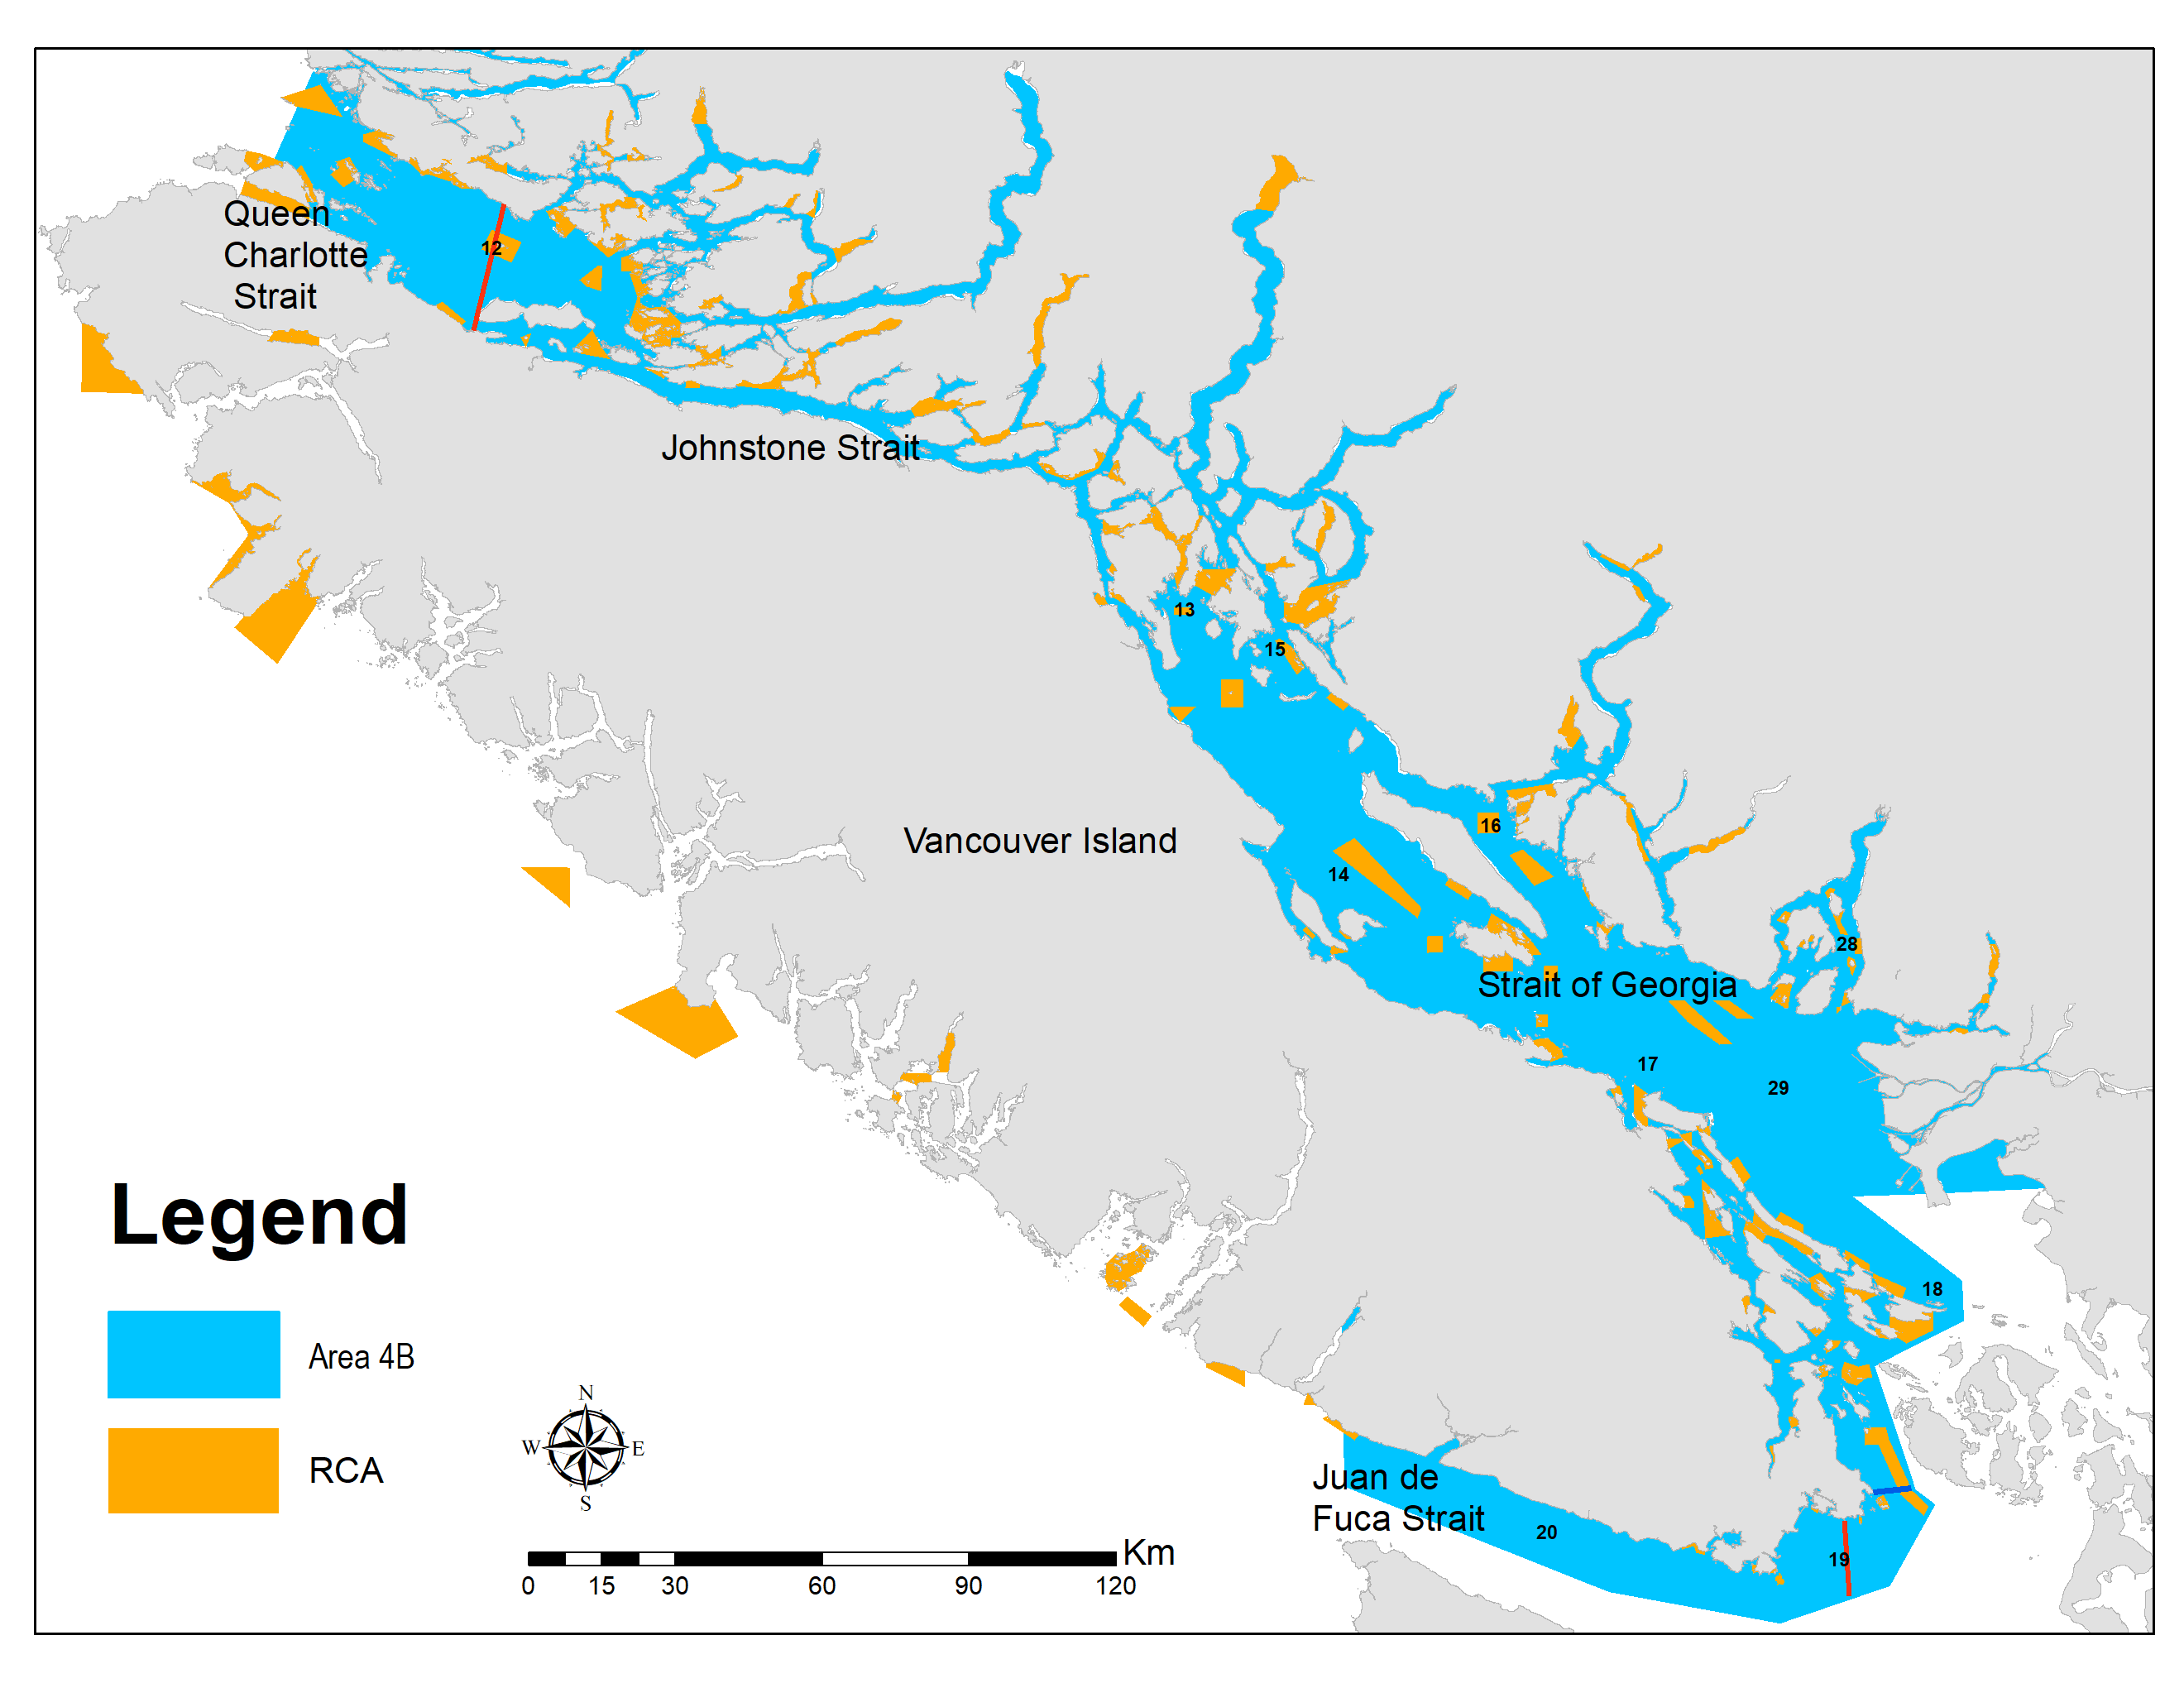
\includegraphics[width=5in]{C:/GitHub/yelloweye-inside/figs/InsideYE_Map_new}}{Figure \ref{fig:map-4B}} 

}

\caption{Map of Groundfish Management Area 4B showing rockfish conservation areas (RCAs) and the boundaries separating the Inside Yelloweye Rockfish designatable unit (DU) from the Outside Yelloweye Rockfish DU. The red lines indicate a proposed adjustment to the range for the Inside DU, based on recent genetic evidence (Siegle \protect\hyperlink{ref-siegle2011}{2011}; Siegle et al. \protect\hyperlink{ref-siegle2013}{2013}; Andrews et al. \protect\hyperlink{ref-andrews2018}{2018}).}\label{fig:map-4B}
\end{figure}
The current rebuilding plan objective is to ``rebuild the stock above the LRP over 80 years with 56\% probability of success''. The milestone objective is to ``achieve positive trends within each 10 year period''. The current MP for Inside Yelloweye Rockfish aims to keep the total annual catch (commercial, recreational, First Nations food, social and ceremonial (FSC), and survey) below 15 tonnes (see Appendix 9 of DFO (\protect\hyperlink{ref-ifmp2018}{2018}) for details).

The guidance for rebuilding plans in Canada states that there should be a high probability of rebuilding fish stocks out of the critical zone within the stated time-frame (DFO \protect\hyperlink{ref-dfo2013}{2013}). Part of the motivation for this project was concern, expressed by fisheries managers, that the 56\% probability of success stated in the current rebuilding plan (DFO \protect\hyperlink{ref-ifmp2018}{2018}) is inconsistent with the definition of high probability.

The guidance document also identifies some recommended management measures, which include: keeping removals from all sources to the lowest possible level; development of a harvest control rule (HCR); and application of management strategy evaluation (MSE) to evaluate, via simulation, the performance of alternative management measures with respect to meeting rebuilding objectives for the stock (DFO \protect\hyperlink{ref-dfo2013}{2013}). The current rebuilding plan implements an annual fixed total allowable catch (TAC) of 15 metric tonnes (DFO \protect\hyperlink{ref-ifmp2018}{2018}), which has not been simulation-tested.

Yelloweye Rockfish are a long-lived species (up to 121 years in B.C., Keppel and Olsen \protect\hyperlink{ref-keppel2019}{2019}), occurring in rocky demersal habitats that have a patchy, discontinuous distribution along BC's inner coast (Yamanaka et al. \protect\hyperlink{ref-yamanaka2011}{2011}). These life history traits make the species vulnerable to overexploitation by fisheries. The inside stock is considered to be data-limited, as there is sparse availability of age-composition data, a lack of biological data from commercial, recreational, and First Nations' fisheries, and uncertainty in the magnitude of historical catches.

\hypertarget{sec:introduction-mse}{%
\subsection{MANAGEMENT STRATEGY EVALUATION (MSE)}\label{sec:introduction-mse}}

Worldwide, the provision of scientific advice for managing fisheries has been moving towards MSE (or management-oriented) approaches (e.g., Butterworth and Punt \protect\hyperlink{ref-butterworth1999}{1999}; Rademeyer et al. \protect\hyperlink{ref-rademeyer2007}{2007}; Berkson and Thorson \protect\hyperlink{ref-berkson2015}{2015}; Geromont and Butterworth \protect\hyperlink{ref-geromont2015}{2015}; Carruthers et al. \protect\hyperlink{ref-carruthers2016}{2016}; Punt et al. \protect\hyperlink{ref-punt2016}{2016}). MSE focuses on identifying MPs that perform best, with respect to meeting agreed-upon policy and fishery objectives, when implemented in a ``closed-loop'' simulation environment (Figure~\ref{fig:mse-chart-basic}). In output-controlled fisheries, such as the quota-managed BC groundfish fishery, MPs describe management measures for setting catch limits. MPs can vary greatly in their data demands, from very data-rich approaches, including statistical catch-at-age stock assessments with harvest control rules, to simple data rules (``data-limited'' approaches), which only rely on catch data and an index of abundance (e.g., Geromont and Butterworth \protect\hyperlink{ref-geromont2015}{2015}; Carruthers et al. \protect\hyperlink{ref-carruthers2016}{2016}).

Closed-loop simulation is distinguished from conventional stock assessment approaches because it simulates feedback between implementation of MPs and the underlying system (the fish stock and its environment), which is described by one or more operating models (OMs). The closed-loop simulation approach takes into account the effect of the MPs on the system, as well as the future data collected from the system and its use in the MPs (Punt et al. \protect\hyperlink{ref-punt2016}{2016}; Carruthers and Hordyk \protect\hyperlink{ref-carruthers2018}{2018}\protect\hyperlink{ref-carruthers2018}{a}; Anderson et al. \protect\hyperlink{ref-anderson2020gfmp}{2020}\protect\hyperlink{ref-anderson2020gfmp}{b}).


\begin{figure}[htb]

{\centering \pdftooltip{\includegraphics[width=6.3in]{C:/GitHub/yelloweye-inside/figs/mse-chart-simple2}}{Figure \ref{fig:mse-chart-basic}} 

}

\caption{Illustration of the fisheries closed-loop simulation process from Anderson et al. (\protect\hyperlink{ref-anderson2020gfmp}{2020}\protect\hyperlink{ref-anderson2020gfmp}{b}) following Punt et al. (\protect\hyperlink{ref-punt2016}{2016}). The management procedure may be based on a simple data rule (e.g., decrease the allowable catch x\% if the survey index decreases y\%) or it might be an estimation model combined with a harvest control rule.}\label{fig:mse-chart-basic}
\end{figure}
\hypertarget{sec:introduction-approach}{%
\subsection{APPROACH}\label{sec:introduction-approach}}

Data-limitations for the Inside Yelloweye stock pose a challenge to evaluating the expected performance of management measures needed to bring the stock into compliance with the Fish Stocks provisions, i.e., to build the stock out of the critical zone within the agreed time-frame and with the agreed probability. Closed-loop simulation-testing of data-limited MPs allows for evaluation of the relative performance of MPs across a range of uncertainties in, for example, underlying fish biology, observation error, estimation error, and implementation error (e.g., Kell et al. \protect\hyperlink{ref-kell2006}{2006}; Carruthers et al. \protect\hyperlink{ref-carruthers2016}{2016}).

Since 2017, a partnership agreement between the University of British Columbia (UBC) and DFO (DFO \protect\hyperlink{ref-dfo_dlmtool_2017}{2017}) has supported development of two open-source software packages for MSE, implemented in the statistical programming environment R (R Core Team \protect\hyperlink{ref-r2019}{2019}): the Data Limited Methods toolkit (DLMtool) (Carruthers and Hordyk \protect\hyperlink{ref-carruthers2018}{2018}\protect\hyperlink{ref-carruthers2018}{a}, \protect\hyperlink{ref-carruthers_hordyk_2018}{2018}\protect\hyperlink{ref-carruthers_hordyk_2018}{b}) and the Management Strategy Evaluation toolkit (MSEtool) (Huynh et al. \protect\hyperlink{ref-huynh_msetool_2019}{2019}). After several years of development, these packages provide some of the fastest, most flexible and extensible software for conducting MSE for fisheries. They can be applied to data-poor or data-rich stocks, enabling rapid assessment of multiple MPs according to customizable conservation and fisheries objectives, and evaluation of key trade-offs.

\hypertarget{sec:introduction-mp-framework}{%
\subsubsection{The Management Procedure Framework for Groundfish in British Columbia}\label{sec:introduction-mp-framework}}

Concurrently with the development of this document, a management procedure framework (MP Framework) for Groundfish in British Columbia (Anderson et al. \protect\hyperlink{ref-anderson2020gfmp}{2020}\protect\hyperlink{ref-anderson2020gfmp}{b}) has been developed for evaluating performance of a wide range of MPs for data-limited groundfish species. The MP Framework uses the functionality of DLMtool and MSEtool extensively, supported by an R package gfdlm (Anderson et al. \protect\hyperlink{ref-gfdlm}{2020}\protect\hyperlink{ref-gfdlm}{d}) written by the authors of Anderson et al. (\protect\hyperlink{ref-anderson2020gfmp}{2020}\protect\hyperlink{ref-anderson2020gfmp}{b}), which houses a suite of software support tools and custom visualizations.

We follow the MP Framework for selecting MPs to set catch limits for data-limited groundfish stocks (Anderson et al. \protect\hyperlink{ref-anderson2020gfmp}{2020}\protect\hyperlink{ref-anderson2020gfmp}{b}). Our evaluation of the Inside Yelloweye rebuilding plan represents the first application of the MP Framework for providing science advice in support of catch decisions. The framework follows six best practice steps described below and in greater detail in Anderson et al. (\protect\hyperlink{ref-anderson2020gfmp}{2020}\protect\hyperlink{ref-anderson2020gfmp}{b}).

The best practice steps are based on a review by Punt et al. (\protect\hyperlink{ref-punt2016}{2016}), who identified five key steps in the MSE process (Steps 2--6 below). An additional first step of the MP Framework, defining the decision context, was identified by Gregory et al. (\protect\hyperlink{ref-gregory2012}{2012}) and Cox and Benson (\protect\hyperlink{ref-cox2016}{2016}). In large part, the DLMtool software has been designed to allow practitioners to follow these steps (Figure~\ref{fig:mse-chart}; Carruthers and Hordyk \protect\hyperlink{ref-carruthers2018}{2018}\protect\hyperlink{ref-carruthers2018}{a}).


\begin{figure}[htb]

{\centering \pdftooltip{\includegraphics[width=\textwidth]{C:/GitHub/yelloweye-inside/figs/mse-chart}}{Figure \ref{fig:mse-chart}} 

}

\caption{The steps of the MSE process following Punt et al. (\protect\hyperlink{ref-punt2016}{2016}) as implemented in DLMtool. Copied from Anderson et al. (\protect\hyperlink{ref-anderson2020gfmp}{2020}\protect\hyperlink{ref-anderson2020gfmp}{b}) and adapted from Carruthers and Hordyk (\protect\hyperlink{ref-carruthers2018}{2018}\protect\hyperlink{ref-carruthers2018}{a}). This figure expands on Figure~\ref{fig:mse-chart-basic}.}\label{fig:mse-chart}
\end{figure}
The six steps are as follows:

Step 1: Definition of the decision context.

Step 2: Selection of objectives and performance metrics.

Step 3: Selection of uncertainties/specification of operating models.

Step 4: Identification of candidate management procedures.

Step 5: Simulation of the application of the management procedures.

Step 6: Presentation of results and selection of management procedure.

After selection and implementation of the MP for setting the catch limit (Figure~\ref{fig:mse-chart}; e.g., applying the selected MP algorithm to the observed survey index), a final necessary step is to periodically monitor and evaluate the performance of the MP (DFO \protect\hyperlink{ref-dfo2013}{2013}; Dowling et al. \protect\hyperlink{ref-dowling2015a}{2015}; Carruthers and Hordyk \protect\hyperlink{ref-carruthers2018}{2018}\protect\hyperlink{ref-carruthers2018}{a}). This may be done through informal means, e.g., via feedback from fishers and survey information (e.g., Cox and Kronlund \protect\hyperlink{ref-cox2008a}{2008}), or through more formal statistical measures, where observed data are compared to predictions from the OMs to test whether the system is performing as expected (Butterworth \protect\hyperlink{ref-butterworth2008}{2008}; Carruthers and Hordyk \protect\hyperlink{ref-carruthers_hordyk_2018}{2018}\protect\hyperlink{ref-carruthers_hordyk_2018}{b}; discussed in Anderson et al. \protect\hyperlink{ref-anderson2020gfmp}{2020}\protect\hyperlink{ref-anderson2020gfmp}{b}).

In the following sections, we describe our approach for developing a candidate rebuilding plan for Inside Yelloweye Rockfish, following the six best practice steps.

\hypertarget{sec:decision-context}{%
\section{DEFINE THE DECISION CONTEXT}\label{sec:decision-context}}

Key questions to guide defining the decision context for MSE include:
\begin{itemize}
\item
  What is the exact decision to be made?
\item
  What is the time frame for making the decision?
\item
  What are specific roles and responsibilities of parties involved? Parties include Science, Management, First Nations, industry, academia, and/or non-governmental organizations (NGOs).
\item
  How will the final decision be made?
\end{itemize}
For this rebuilding plan, the decision to be made is which MP to use to determine catch limits for the period until the next available catch advice. The final decision on the MP to determine future catch limits should be made based on a consensus by the Regional Peer Review (RPR) committee, after review of the scientific content of the advice (including the structure and content of the OMs), and consideration of the relative performance of the MPs and trade-offs among performance metrics.

\hypertarget{sec:objectives-metrics}{%
\section{SELECTION OF OBJECTIVES AND PERFORMANCE METRICS}\label{sec:objectives-metrics}}

Clear management and fishery objectives must be identified, along with the performance metrics that measure them. Objectives may span a wide range of policy or legislated objectives (e.g., maintaining the stock above the LRP), economic objectives (e.g., maintaining an average catch or reducing variability in catch), and cultural objectives (e.g., maintaining minimum required access to the stock or specific fishing areas). In a rebuilding scenario, conservation objectives must take precedence. However, in a simulation framework it is possible to examine trade-offs between conservation and other short and long-term fishery objectives, so long as the primary conservation objective is met. Fully quantified objectives include a metric or target, the desired probability of success, and a time frame to achieve the objective (e.g., probability of maintaining the stock above the LRP is greater than 0.95 {[}19 times out of 20{]}, over 1.5 generations of the stock). Performance metrics are quantified measures of the objectives. In closed-loop simulation, they are calculated in the OM at each time step of the projections.

The original rebuilding plan objective was to rebuild the stock above the LRP over 80 years with 56\% probability of success. An additional milestone objective was to achieve positive biomass trends within each 10 year period. The MP that was agreed upon to meet these objectives was to maintain the combined TAC (commercial, recreational, FSC, biological survey) below 15 tonnes annually (DFO \protect\hyperlink{ref-ifmp2018}{2018}).

\hypertarget{sec:objectives-metrics-obj}{%
\subsection{OBJECTIVES AND MILESTONES}\label{sec:objectives-metrics-obj}}

We present a set of refined objectives and associated performance metrics for the rebuilding plan for Inside Yelloweye Rockfish. Key provisional conservation objectives are guided by the PA Framework (DFO \protect\hyperlink{ref-dfo2006}{2006}, \protect\hyperlink{ref-dfo2009}{2009}), the rebuilding plan guidance document (DFO \protect\hyperlink{ref-dfo2013}{2013}), and regional precedents (Cox et al. \protect\hyperlink{ref-cox2019}{2019}, \protect\hyperlink{ref-cox2020}{2020}). Additional objectives related to fisheries yield and variability in annual fisheries yield are based on precedents in other DFO Pacific Region analyses (e.g., Cox and Kronlund \protect\hyperlink{ref-cox2008a}{2008}; Forrest et al. \protect\hyperlink{ref-forrest2018}{2018}; Cox et al. \protect\hyperlink{ref-cox2019}{2019}, \protect\hyperlink{ref-cox2020}{2020}).

The proposed core conservation objective is:
\begin{enumerate}
\def\labelenumi{\arabic{enumi}.}

\item
  Rebuild the stock above the LRP over 56 years (1.5 generations) with at least 95\% {[}19 times out of 20{]} probability of success.
\end{enumerate}
We adjusted the original rebuilding time-frame of 80 years (DFO \protect\hyperlink{ref-ifmp2018}{2018}) to 56 years in this analysis, based on the estimated generation time for outside Yelloweye Rockfish (Cox et al. \protect\hyperlink{ref-cox2020}{2020}), reflecting the guidance that rebuilding should be achieved within 1.5 to 2 generation times (DFO \protect\hyperlink{ref-dfo2013}{2013}). For more information on generation time, please see Appendix~\ref{app:biological-data}, Section~\ref{sec:generation}. The desired probability of success was increased from 56\% to 95\% to reflect rebuilding guidance that the probability of rebuilding should be high, and international best practice, where policies in numerous jurisdictions aim to keep stocks above the LRP with 90-95\% probability {[}18 to 19 times out of 20{]}(Sainsbury \protect\hyperlink{ref-sainsbury2008}{2008}; McIlgorm \protect\hyperlink{ref-mcilgorm2013}{2013}).

We also propose the following additional objectives, further specified in Section~\ref{sec:objectives-metrics-pm}:
\begin{enumerate}
\def\labelenumi{\arabic{enumi}.}
\setcounter{enumi}{1}
\item
  Rebuild the stock above the USR over 56 years (1.5 generations).
\item
  Rebuild the stock above the LRP over 38 years (1 generation).
\item
  Given the above conservation objectives are achieved, maintain an average target catch in the short and long term.
\item
  Given the above conservation objectives are achieved, minimize variability in fisheries catch from year to year.
\end{enumerate}
Note that we did not assign target probabilities to these objectives as they are provided for the purpose of evaluating trade-offs with Objective 1. However, we screened out MPs that did not meet a minimum probability of maintaining catch above 10 t in the short-term (see Section~\ref{sec:simulation}).

In addition to the above objectives, we propose refining the milestones identified in the original rebuilding plan (DFO \protect\hyperlink{ref-ifmp2018}{2018}) with the italicized text as follows:
\begin{enumerate}
\def\labelenumi{\arabic{enumi}.}
\setcounter{enumi}{5}

\item
  Achieve positive biomass trends within each 10 year period \emph{for as long as the stock remains below the LRP}.
\end{enumerate}
The 10 year period identified in the milestones for the current Inside Yelloweye rebuilding plan (DFO \protect\hyperlink{ref-ifmp2018}{2018}) reflected an assumption that rebuilding out of the critical zone could be very slow for this stock. We adjusted the milestone to reflect the assumption that, once the stock is no longer in the critical zone, the milestone would no longer be required. The current rebuilding guidance (DFO \protect\hyperlink{ref-dfo2013}{2013}) only provides for objectives to build stocks out of the critical zone, with milestones intended to ensure progress is achieved during the rebuilding process. The guidance does discuss having longer-term objectives to keep rebuilding stocks into the healthy zone, above the USR. However, this is supposed to be achieved beyond the period and scope of the rebuilding plan (DFO \protect\hyperlink{ref-dfo2013}{2013}).

\hypertarget{sec:objectives-metrics-pm}{%
\subsection{PERFORMANCE METRICS}\label{sec:objectives-metrics-pm}}

We propose the following performance metrics to measure the objectives, where \emph{B} represents spawning biomass, MSY refers to maximum sustainable yield, \emph{B}\textsubscript{MSY} refers to equilibrium spawning biomass at MSY, GT represents generation time, and AADC represents average absolute deviation in catch (\(C\)) over \(n\) years (note: \emph{ST} = short term, \emph{LT} = long term). We define the LRP and USR as 0.4\emph{B}\textsubscript{MSY} and 0.8\emph{B}\textsubscript{MSY}, respectively, following the provisional definitions in the PA Framework (DFO \protect\hyperlink{ref-dfo2006}{2006}), as used in the 2010 stock assessment (Yamanaka et al. \protect\hyperlink{ref-yamanaka2011}{2011}). In the closed-loop simulations, all reference points and performance metrics are calculated in the OM. Raw performance metrics are calculated in each of the 100 years of the projection period and summarized according to the time-frame of interest:
\begin{enumerate}
\def\labelenumi{\arabic{enumi}.}

\item
  \textbf{LRP 1.5GT}: P(\emph{B} \textgreater{} 0.4 \emph{B}\textsubscript{MSY}) after 1.5 GT (in 2075, year 56 of the projection period)
\item
  \textbf{USR 1.5GT}: P(\emph{B} \textgreater{} 0.8 \emph{B}\textsubscript{MSY}) after 1.5 GT (in 2075, year 56 of the projection period)
\item
  \textbf{LRP 1GT}: P(\emph{B} \textgreater{} 0.4 \emph{B}\textsubscript{MSY}) after 1 GT (in 2057, year 38 of the projection period)
\item
  \textbf{ST C10}: P(average catch \textgreater{} 10 t) during 2020--2029, years 1--10 of the projection period\\
\item
  \textbf{ST C15}: P(average catch \textgreater{} 15 t) during 2020--2029, years 1--10 of the projection period 
\item
  \textbf{LT C20}: P(average catch \textgreater{} 20 t) after 1 GT (in 2057, year 38 of the projection period)
\item
  \textbf{ST AADC}: P(AADC\textsubscript{2020--2029} \textless{} AADC\textsubscript{2012--2019})
\end{enumerate}
We included the performance metric LRP 1 GT as a check that the MPs do not crash the stock in the short term. We selected 10 t, 15 t and 20 t as catch targets, representing catch levels spanning 5 t below and above the current 15 t TAC.

We calculated AADC\textsubscript{2020--2029} as:
\begin{equation}
\textrm{AADC}_\textrm{2020-2029} = \dfrac{1}{9}\sum_{y=2021}^{2029} \mid C_y - C_{y-1} \mid.
\end{equation}
A baseline period (2012--2019) was selected because it is the period since the start of the 15 t TAC. We calculated AADC\textsubscript{2012--2019} as:
\begin{equation}
\textrm{AADC}_\textrm{2012-2019} = \dfrac{1}{7}\sum_{y=2013}^{2019} \mid C_y - C_{y-1} \mid.
\end{equation}
In cases where performance metrics are calculated over a range of years, care needs to be taken to clearly report how summary statistics are calculated. Anderson et al. (\protect\hyperlink{ref-anderson2020gfmp}{2020}\protect\hyperlink{ref-anderson2020gfmp}{b}) provisionally suggested calculating performance statistics across replicates and years for the entire time window defined for the performance metric. We follow this protocol here. For example, we averaged the short-term catch metrics over replicates and the years 2020--2029.

\hypertarget{sec:om}{%
\section{SELECTION OF UNCERTAINTIES/SPECIFICATION OF OPERATING MODELS}\label{sec:om}}

DLMtool OMs are organized into four main components representing a real fished system:
\begin{enumerate}
\def\labelenumi{\arabic{enumi}.}

\item
  population dynamics of the fish stock (e.g., growth, recruitment, mortality);
\item
  fishery dynamics (e.g., selectivity, spatial targeting);
\item
  observation processes (e.g., bias and precision in survey indices); and
\item
  management implementation (e.g., catch limit overages).
\end{enumerate}
Equations and parameters describing the four OM components are provided in detail in Appendix B of Carruthers and Hordyk (\protect\hyperlink{ref-carruthers2018}{2018}\protect\hyperlink{ref-carruthers2018}{a}) and Appendix A of Anderson et al. (\protect\hyperlink{ref-anderson2020gfmp}{2020}\protect\hyperlink{ref-anderson2020gfmp}{b}). DLMtool allows the incorporation of uncertainty in many OM parameters through optional specification of probability distributions. To further isolate the effects of specific sources of uncertainty on performance of MPs, we develop alternative OMs that change the value (or distribution) of one or more parameters and/or data sources of interest (Section~\ref{sec:approach3-oms}).

Best practice recommends calibrating or conditioning OMs with observed data, so they can reproduce historical observations. DLMtool's companion software package, MSEtool (Huynh et al. \protect\hyperlink{ref-huynh_msetool_2019}{2019}), includes an efficient implementation of a stock reduction analysis (SRA) (Kimura and Tagart \protect\hyperlink{ref-kimura1982}{1982}; Walters et al. \protect\hyperlink{ref-walters2006}{2006}), which is effectively a statistical catch-at-age model that estimates the combinations of historical fishing mortality and recruitment that would be consistent with the observed data. The SRA is fully described in Appendix B of Anderson et al. (\protect\hyperlink{ref-anderson2020gfmp}{2020}\protect\hyperlink{ref-anderson2020gfmp}{b}).

There are two distinct time-periods in the simulation framework: (1) the historical period, which includes all years from the first year of the observed catch time series \(t_1\) to the final year of the observed catch time series \(t_c\) (where ``c'' represents the ``current'' year); and (2) the projection period, which covers the period from the first year after \(t_c\) to the final projection year \(t_N\). The historical period is conditioned on historical observations using the SRA (see Appendix B of Anderson et al. \protect\hyperlink{ref-anderson2020gfmp}{2020}\protect\hyperlink{ref-anderson2020gfmp}{b}). The closed-loop simulations, with application of the MPs and calculation of performance metrics, begin in the first year of the projection period (year \(t_{c+1}\)).

OM development in the MP Framework follows three steps:
\begin{enumerate}
\def\labelenumi{\arabic{enumi}.}
\item
  Set parameter values and ranges in the OM.
\item
  Pass the OM parameters to the SRA model, which conditions the OM by fitting to historical observed catches, indices of abundance, and any available years of age-composition data. This results in conditioned estimates of model parameters and estimates of historical biomass and historical fishing mortality (in years \(t_1\) to \(t_c\)), which are consistent with historical observations.
\item
  Pass the conditioned parameter values back to the OM (now the ``conditioned'' OM) for use in the closed-loop simulation projections, starting in year \(t_{c+1}\).
\end{enumerate}
Where possible, we derived OM settings from all available survey biological data from area 4B, which is primarily collected on the inside hard bottom longline (HBLL) surveys (Appendix~\ref{app:biological-data}). We derived other parameters from the scientific literature and stock assessments for Yelloweye Rockfish in other areas (see Appendix~\ref{app:desc-om-yelloweye} for details). A list of ``default'' OM parameter settings recommended for most BC groundfish stocks is provided in Appendix C of Anderson et al. (\protect\hyperlink{ref-anderson2020gfmp}{2020}\protect\hyperlink{ref-anderson2020gfmp}{b}).

We conditioned the OMs with the SRA, using age-composition data from research surveys (Appendix~\ref{app:biological-data}), inside HBLL survey indices (Appendix~\ref{app:index-data}), and commercial and recreational catch data (Appendix~\ref{app:catch-data}). Results from conditioning the OMs are provided below in Section~\ref{sec:approach3-conditioning}.

\hypertarget{sec:approach3-oms}{%
\subsection{OPERATING MODELS}\label{sec:approach3-oms}}

MSE best practice recommends dividing MSE trials into a ``reference set'' of core OMs that include the most important uncertainties (e.g., depletion of the stock or range of natural mortality values), and a ``robustness set'', to capture a wider range of uncertainties that may be less plausible but should nonetheless be explored (Rademeyer et al. \protect\hyperlink{ref-rademeyer2007}{2007}). Anderson et al. (\protect\hyperlink{ref-anderson2020gfmp}{2020}\protect\hyperlink{ref-anderson2020gfmp}{b}) recommended presenting performance metrics from the reference and robustness sets separately. They recommended that, for most results, reference set performance metrics should be averaged across all OM reference set scenarios (an ensemble approach to integrate across OM uncertainties) but that performance metrics from individual OM robustness set scenarios should be presented separately. Presenting robustness results separately allows managers to see how MPs that performed well in the reference set perform under a set of more diverse assumptions (Rademeyer et al. \protect\hyperlink{ref-rademeyer2007}{2007}).

For Inside Yelloweye Rockfish, we established four reference set OMs: (1) a baseline OM; (2) an OM reflecting an alternative assumption about the magnitude of historical catch during the period 1986--2005; (3) an OM allowing for episodic (rare but large) future recruitment events; and (4) an OM estimating selectivity in the HBLL survey (Table~\ref{tab:ye-scen}).

We further established two robustness set OMs encompassing additional sources of uncertainty: (A) an OM that assumes lower natural mortality than the other OMs; and (B) an OM that assumes a higher coefficient of variation (CV) in the future HBLL survey (Table~\ref{tab:ye-scen}).
\begin{longtable}[]{@{}ll@{}}
\caption{\label{tab:ye-scen}Inside Yelloweye Rockfish OM scenarios.}\tabularnewline
\toprule
OM Scenario name & Set type\tabularnewline
\midrule
\endfirsthead
\toprule
OM Scenario name & Set type\tabularnewline
\midrule
\endhead
(1) Base & Reference\tabularnewline
(2) Low catch & Reference\tabularnewline
(3) Episodic recruitment & Reference\tabularnewline
(4) Estimate HBLL selectivity & Reference\tabularnewline
(A) Low M & Robustness\tabularnewline
(B) High HBLL CV & Robustness\tabularnewline
\bottomrule
\end{longtable}
\hypertarget{sec:approach3-reference}{%
\subsubsection{Reference set}\label{sec:approach3-reference}}

The following OMs were developed as the reference set. We hereafter refer to them by their numbers, e.g., OM Scenario (1).

\hypertarget{sec:approach3-reference1}{%
\subsubsection{(1) Base}\label{sec:approach3-reference1}}

Data sources are provided in Appendices~\ref{app:biological-data} through~\ref{app:catch-data}. Parameter settings for the Base OM are provided in Appendix~\ref{app:desc-om-yelloweye}. We here provide a brief description of the Base OM assumptions that were adjusted in other OM scenarios.

There are two main uncertainties associated with the historical commercial catch time series for Inside Yelloweye Rockfish (details in Appendix~\ref{app:catch-data}, Section~\ref{sec:com-catch-data}). These are: (1) aggregated reporting of rockfish as Other Rockfish (ORF; rockfish species other than Pacific Ocean Perch) and (2) the magnitude of unreported catch that was discarded at sea prior to the introduction of 100\% at-sea monitoring in the groundfish longline fleet in 2006 (Stanley et al. \protect\hyperlink{ref-stanley2009}{2009}). For consistency with Yamanaka et al. (\protect\hyperlink{ref-yamanaka2011}{2011}), we doubled the nominal catch data for the period 1986---2005, as industry did not have confidence in the catch data for those years {[}DFO (\protect\hyperlink{ref-dfo2012}{2012}\protect\hyperlink{ref-dfo2012}{a}); see Appendix~\ref{app:catch-data}, Section~\ref{sec:com-catch-data}{]}.

Projected recruitment deviations were sampled in log space with standard deviation \(\tau = 0.4\), with autocorrelation estimated post-hoc from the historical recruitment deviates in the SRA model (Appendix A of Anderson et al. \protect\hyperlink{ref-anderson2020gfmp}{2020}\protect\hyperlink{ref-anderson2020gfmp}{b}).

The Inside Yelloweye Rockfish stock is indexed by two fishery-independent surveys: the inside Hard Bottom Longline Survey (Appendix~\ref{app:index-data}, Section~\ref{sec:hbll-index-data}) and the Dogfish Survey (Appendix~\ref{app:index-data}, Section~\ref{sec:dogfish-index-data}). The SRA model exhibited better retrospective behaviour when the SRA model was fit with more likelihood weight applied to the Dogfish Survey. The age of full selectivity in the HBLL survey was fixed at 22 years (see Section~\ref{sec:approach3-conditioning} below).

Historical commerical CPUE was also available and used as an index of abundance for conditioning the OM (Yamanaka et al. \protect\hyperlink{ref-yamanaka2011}{2011}). Following the decisions made for the 2011 assessment, the time series was divided into three stanzas (1986-1990, 1995-2001, and 2003-2005), representing periods when fishery behaviour is likely to have changed in response to management regulations (Appendix~\ref{app:catch-data}, Section~\ref{sec:management-changes}).

Natural mortality (\emph{M}) was sampled from a probability distribution based on that used by Yamanaka et al. (\protect\hyperlink{ref-yamanaka2011}{2011}), where \(M \sim \textrm{Lognormal}(0.045, 0.2)\) (Appendix~\ref{app:desc-om-yelloweye}, Section~\ref{app:desc-stock-m-yelloweye}).

During the projection period, only the HBLL index was assumed to be available for the MPs, as this survey is conducted annually. Projecting only one index of abundance is consistent with many data-limited MPs, which only use a single index of abundance (see Appendix~\ref{app:mps}). Observation error in the projected index values was simulated with random deviates from a lognormal distribution with mean of 1 and standard deviation of 0.25 based on the estimated observation error in the HBLL index.

All other OM scenarios were adjusted from this baseline OM and differed only in terms of adjustments to key parameters or data sources, described below.

\hypertarget{sec:approach3-reference2}{%
\subsubsection{(2) Low catch}\label{sec:approach3-reference2}}

In the ``Low catch'' OM scenario, we test model sensitivity to the assumption of large unreported catch for the period 1986--2005. Instead of doubling nominal catch data for this period, the SRA was fit to the nominal catch data. As for the other OM scenarios, we used the reconstructed catch up to 1985 and the nominal catch from 1986 onwards.

\hypertarget{sec:approach3-reference3}{%
\subsubsection{(3) Episodic recruitment}\label{sec:approach3-reference3}}

Long-lived, late-maturing species such as Pacific rockfishes often exhibit episodic, or periodic, recruitment strategies characterized by high fecundity and occasional very large recruitment events (Winemiller and Rose \protect\hyperlink{ref-winemiller1992}{1992}; Rose et al. \protect\hyperlink{ref-rose2001}{2001}; Winemiller \protect\hyperlink{ref-winemiller2005}{2005}). This life history strategy is sometimes called the storage effect (Warner and Chesson (\protect\hyperlink{ref-warner1985}{1985})) because strong recruitment events are stored in the adult population and are capable of contributing to reproduction, sometimes significantly, when favourable conditions return. Longevity in rockfish is thought to have evolved as a strategy for weathering un-favourable conditions. Very large or even extreme year classes have been observed for several BC rockfish species (e.g., Pacific Ocean Perch: Haigh et al. \protect\hyperlink{ref-haigh2019}{2019}; Bocaccio: Haigh and Starr \protect\hyperlink{ref-haigh2020}{2020}).

To address the possibility that future recruitment during the projection period could be characterized by occasional very large recruitment events, we included an ``Episodic recruitment'' OM scenario. This OM scenario addresses the concern that very large cohorts are not adequately modelled by the lognormal distribution for recruitment deviations that was used in OM Scenario (1). In the Episodic recruitment OM scenario, recruitment deviations \(\varepsilon_{R,y}\) for each year of the projection period are generated as:
\begin{equation}
\varepsilon_{R,y} = 
\left\{
\begin{array}{ll}
\varepsilon^{(1)}_{R,y} & \eta_y = 0\\
\varepsilon^{(3)}_{R,y} & \eta_y = 1,
\end{array}
\right.
\end{equation}
where \(\varepsilon^{(1)}_{R,y}\) is the recruitment deviation from OM Scenario (1) and \(\log\varepsilon^{(3)}_{R,y} \sim \textrm{Normal}(-0.5\tau^2, \tau)\) represents the ``episodic'' recruitment distribution with \(\tau = 2\) (standard deviation). The parameter \(\eta_y\) is a Bernoulli random variable \(\eta_y \sim \textrm{Bernoulli}(p = 1/38)\), which selects whether an extreme recruitment event will occur. We assume that an extreme recruitment event is expected to occur once every generation (38 years), based on the observation that strong recruitment events in Inside Yelloweye Rockfish were present in 1948 and 1970. Although recent environmental conditions may be favourable for some species of rockfishes (Haigh and Starr \protect\hyperlink{ref-haigh2020}{2020}; Lincandeo et al. \protect\hyperlink{ref-lincandeo2020}{2020}), we don't yet have any evidence of recent strong recruitment events for Inside Yelloweye Rockfish that might indicate more frequent episodic or spasmodic recruitment events.

\hypertarget{sec:approach3-reference4}{%
\subsubsection{(4) Estimate HBLL selectivity}\label{sec:approach3-reference4}}

Annual sample sizes of age-composition data from research surveys are very small (Appendix~\ref{app:biological-data}). This makes estimation of selectivity in the surveys highly uncertain, which led to the choice to fix survey selectivity in the other OM scenarios.

Given large uncertainty in our choice of selectivity, we allowed the SRA to estimate selectivity for the surveys in this OM scenario and utilized the available survey age-composition data.

\hypertarget{sec:approach3-robustness}{%
\subsubsection{Robustness set}\label{sec:approach3-robustness}}

The following OMs were developed as the robustness set. We hereafter refer to them by their letters.

\hypertarget{sec:approach3-referenceA}{%
\subsubsection{(A) Low M}\label{sec:approach3-referenceA}}

Lower values of natural mortality have been used for Inside Yelloweye Rockfish (Yamanaka and Lacko \protect\hyperlink{ref-yamanaka2001}{2001}; COSEWIC \protect\hyperlink{ref-cosewic2008}{2008}\protect\hyperlink{ref-cosewic2008}{a}; Wood et al. \protect\hyperlink{ref-wood2019}{2019}). This OM scenario used a lower mean in the distribution for \emph{M}, with \(M \sim \textrm{Lognormal}(0.025, 0.2)\), reflecting the possibility that the stock could be less productive than assumed in the other OM scenarios.

\hypertarget{sec:approach3-referenceB}{%
\subsubsection{(B) Higher HBLL CV}\label{sec:approach3-referenceB}}

This OM scenario considers the possibility that the future HBLL index might be less precise than assumed in the other OM scenarios. Instead of an observation standard deviation \(\sigma_I = 0.25\), we use the standard deviation (\(\sigma_I\)) and autocorrelation (\(\theta_\textrm{AC}\)) from the index residuals in OM Scenario (1), obtained from the SRA fit to the HBLL index.

This \(\sigma_I\) has a mean of 0.41 and a range of 0.38--0.44.

\hypertarget{sec:approach3-conditioning}{%
\subsection{CONDITIONING THE OPERATING MODELS}\label{sec:approach3-conditioning}}

After specifying the OM parameters (Appendix~\ref{app:desc-om-yelloweye}), we conditioned the OMs using the SRA model described in Appendix B of Anderson et al. (\protect\hyperlink{ref-anderson2020gfmp}{2020}\protect\hyperlink{ref-anderson2020gfmp}{b}).

Note that the DLMtool OM combines all fleets into a single fleet. However, if the OM is conditioned using the SRA model, the SRA can accommodate multiple fleets, and selectivity is fleet-specific. In this case, fishery selectivity in the OM for the projection period is replaced with the SRA-conditioned estimates of fishing mortality-at-age in the final year of the historical period (\(t_c\)), normalized by dividing by apical fishing mortality in that year. This essentially provides the DLMtool OM with relative selectivity-at-age, weighted by catch across all fleets. The closed-loop simulation projections therefore assume that the relative selectivity across fleets remains constant in the projection period.

Similarly, if the OM is conditioned using the SRA model, analysts can also specify (or estimate) selectivity parameters for the individual indices of abundance (in this case two fishery-independent surveys and three commercial CPUE series (Figure~\ref{fig:survey-fits})). In this case, the SRA passes all of the indices back to DLMtool, preserving the estimated or user-defined selectivities-at-age for each index. However, note that the DLMtool MPs only utilize a single index of abundance (see Appendix~\ref{app:mps}). In the current study, all index-based MPs utilize the inside HBLL survey.

We used the SRA to populate the following parameters in the conditioned OMs:
\begin{itemize}

\item
  \(B_{t_c}/B_0\) (or ``D''; depletion in the last historical year \(t_c\))
\item
  \(R_0\) (unfished recruitment)
\item
  \(\theta_\textrm{AC}\) (or ``AC''; first-order autocorrelation of recruitment deviations)
\item
  \(\varepsilon_{\textrm{R},y}\) for years \(t_1\) to \(t_c\) (annual recruitment deviations)
\item
  \(F_{a,y}\) (fishing mortality at age by year)
\end{itemize}
See Appendix B of Anderson et al. (\protect\hyperlink{ref-anderson2020gfmp}{2020}\protect\hyperlink{ref-anderson2020gfmp}{b}) for details on these parameters.

The SRA was run for 250 replicates. Each replicate used a different value of \emph{M} and \emph{h} (sampled independently from the distributions shown in Appendix~\ref{app:desc-om-yelloweye}, except for OM Scenario (A), which used a different distribution for \emph{M}). The model was initialized under the assumption that spawning biomass (\(B_y\)) was in an unfished equilibrium state prior to 1918, the first year of the time series, i.e., \(B_{1918} = B_0\). While this is unlikely to be true, as First Nations and others would have been catching Yelloweye Rockfish prior to 1918, these numbers are expected to be small enough not to impact the outcomes of the performance of MPs in the projection period.

\hypertarget{sec:approach3-conditioning-base-om}{%
\subsubsection{Selection of base OM}\label{sec:approach3-conditioning-base-om}}

Initial attempts to fit the SRA model did not produce good fits to the dogfish survey. Furthermore, retrospective analysis showed persistent retrospective bias in annual estimates of spawning biomass when sequentially removing 11 years of data (when evaluated at the mean values of \emph{M} and \emph{h}, Figure~\ref{fig:retro-initial}, top panel). The choice to base retrospective analysis on 11 years of data was primarily to evaluate sensitivity of the model to removal of each year of data, going back to 2009, the terminal year for the 2011 assessment.

Increasing the likelihood weight for the SRA fit to the Dogfish survey (\(\lambda^I_s = 4\); Equation B.22 in Anderson et al. \protect\hyperlink{ref-anderson2020gfmp}{2020}\protect\hyperlink{ref-anderson2020gfmp}{b}), and fixing age-at-full-selectivity in the HBLL survey to 22 years, removed the retrospective pattern (Figure~\ref{fig:retro-initial}, bottom panel). Therefore, for OM Scenario (1) and all other OM scenarios except Scenario (4), we fixed the age-at-full selectivity of the HBLL Survey at 22 years (Figure~\ref{fig:HBLL-selectivity}), while also upweighting the Dogfish survey.


\begin{figure}[htb]

{\centering \pdftooltip{\includegraphics[width=4.25in]{C:/GitHub/yelloweye-inside/mse/figures/retrospective-spawning-biomass}}{Figure \ref{fig:retro-initial}} 

}

\caption{Retrospective patterns in spawning biomass for the initial fit and OM Scenario (1). Coloured lines represent estimates of spawning biomass with \(X\) years of data removed, where \(X\) is shown in the legend for each series.}\label{fig:retro-initial}
\end{figure}
There are a number of factors that increase uncertainty in estimating selectivity for the Dogfish survey e.g.~the absence of biological data from this survey, and changes in fishing operations and hook type that occurred in 2004 (Appendix~\ref{app:index-data}, Section~\ref{sec:dogfish-index-data}). There are also several differences between the HBLL and Dogfish longline surveys (Appendix~\ref{app:index-data}, Section~\ref{sec:dogfish-index-data}), but, for the reasons mentioned, we cannot reliably estimate the selectivity for the Dogfish survey. Out of necessity, selectivity in the Dogfish survey was set to mirror selectivity in the HBLL survey, whether it was estimated (OM Scenario (4)) or fixed (all other OM scenarios).

Age composition data from the commerical fishery were available from a single fishing trip in 1989, and length samples from 2002--2019 were identified from the recreational fishery. Attempts to fit the SRA model to these data did not produce satisfactory estimates of selectivity. The estimated values of the age of full selectivity were very high, suggesting that most ages were not completely vulnerable to the fishery, and significantly differed from values estimated for the Outside Yelloweye population (Cox et al. \protect\hyperlink{ref-cox2020}{2020}). Since it is unlikely that selectivity varies to such an extent between geographical regions, these data were not further considered.

As a result, selectivity for these gears was fixed in all OM scenarios (Figure~\ref{fig:sra-selectivity}). Parameter values were set so that the selectivity-at-age curves approximated those estimated by Cox et al. (\protect\hyperlink{ref-cox2020}{2020}) for the commercial longline and recreational fisheries for outside Yelloweye Rockfish (see Appendix~\ref{app:desc-om-yelloweye}, Section~\ref{app:desc-fleet-selectivity-yelloweye}). As noted above, these selectivities were returned to the DLMtool OMs as a combined-fleet selectivity curve from the terminal year (\(t_c\)) of the historical period (Figure~\ref{fig:om-selectivity}).

\hypertarget{sec:approach3-conditioning-results}{%
\subsubsection{OM conditioning results}\label{sec:approach3-conditioning-results}}

The following sections describe the results of conditioning the OMs.

\hypertarget{sec:approach3-conditioning-indices}{%
\subsubsection{Fits to data}\label{sec:approach3-conditioning-indices}}

The predicted catch in the SRA models matched the catch data by design, which was achieved by setting the standard deviation of the observation error to a value of 0.01 (Anderson et al. \protect\hyperlink{ref-anderson2020gfmp}{2020}\protect\hyperlink{ref-anderson2020gfmp}{b}, their Equation B.27).

The SRA was able to fit to the indices of abundance reasonably well (Figure~\ref{fig:survey-fits}) and convergence was achieved for all replicates in all OM scenarios. For all OM scenarios, the estimated index fell within the observed confidence intervals in most years, although there were some outliers (Figure~\ref{fig:survey-fits}). The fit to the early 1986 and 1989 observations in the Dogfish Survey was slightly better in OM Scenario (A), which is consistent with a less productive, more depleted stock. However, these two observations are more uncertain than those in recent years, due to changes in fishing operations and hook type that occurred in 2004 (Appendix~\ref{app:index-data}, Section~\ref{sec:dogfish-index-data}). Fits to the commercial CPUE series were generally good, due to the short time stanzas for each series (Figure~\ref{fig:survey-fits}).


\begin{figure}[htb]

{\centering \pdftooltip{\includegraphics[width=\textwidth]{C:/GitHub/yelloweye-inside/mse/figures/ye-index-fits}}{Figure \ref{fig:survey-fits}} 

}

\caption{SRA model fits to the HBLL, Dogfish, and three commercial CPUE relative indices. Panels from left to right represent OM scenarios. Thin lines represent individual SRA model fits across stochastic draws from the various OM parameters. Dots represent index mean and line segments represent 2 times the standard errors as entered into the SRA models.}\label{fig:survey-fits}
\end{figure}
The SRA model fit the survey age-composition data reasonably well, despite very small sample sizes (Figures~\ref{fig:sra-conditioned-comp-fit1} to~\ref{fig:sra-conditioned-comp-fitB}). We note that in comparing OM Scenarios (1) and (4) it appears that fixing or estimating selectivity in the HBLL survey did not generate very different fits to the age composition data (Figures~\ref{fig:sra-conditioned-comp-fit1} and~\ref{fig:sra-conditioned-comp-fit4}).

For most years, the SRA predicted larger abundance in the plus group (80+ \emph{y}) than what was observed. A lack of fish older than 80 \emph{y} in the survey suggested that total mortality could have been greater in the past than estimated in our OMs. This could be represented in the OMs in two ways. First, \emph{M} could be increased in the models. However, our preliminary model investigations indicated that increasing \emph{M} also increases retrospective bias. Secondly, the catch history could be changed to predict higher values of fishing mortality. This was done in OM Scenario (2) by assuming lower catches in 1986-2005, which resulted in a slightly smaller stock (Figure~\ref{fig:biomass-om}) and higher fishing mortality (Figure~\ref{fig:F-om}). However, the estimated plus group was only slightly reduced in most years for this OM scenario (Figure~\ref{fig:sra-conditioned-comp-fit2}).

This issue is a challenge for very long-lived species with poor age-composition sampling. With such small sample sizes, there is a relatively small chance of observing very old fish. Large structural uncertainties in the model and available data (e.g., the Dogfish survey, catch data) made it difficult to resolve one issue, e.g., persistent overprediction of old fish, without generating another issue, e.g., retrospective bias.

\clearpage


\begin{figure}[htb]

{\centering \pdftooltip{\includegraphics[width=0.85\textwidth]{C:/GitHub/yelloweye-inside/mse/figures/conditioning/HBLL_age_comp_updog_fixsel}}{Figure \ref{fig:sra-conditioned-comp-fit1}} 

}

\caption{SRA model fits to the survey age composition data for OM Scenario (1), showing observed (points) and estimated (green lines) proportions. Sample sizes (N) are number of sets from which age samples were collected in each year.}\label{fig:sra-conditioned-comp-fit1}
\end{figure}
\clearpage


\begin{figure}[htb]

{\centering \pdftooltip{\includegraphics[width=0.85\textwidth]{C:/GitHub/yelloweye-inside/mse/figures/conditioning/HBLL_age_comp_lowcatch_fixsel}}{Figure \ref{fig:sra-conditioned-comp-fit2}} 

}

\caption{SRA model fits to the survey age composition data for OM Scenario (2), showing observed (points) and estimated (green lines) proportions. Sample sizes (N) are number of sets from which age samples were collected in each year.}\label{fig:sra-conditioned-comp-fit2}
\end{figure}
\clearpage


\begin{figure}[htb]

{\centering \pdftooltip{\includegraphics[width=0.85\textwidth]{C:/GitHub/yelloweye-inside/mse/figures/conditioning/HBLL_age_comp_episodic_recruitment}}{Figure \ref{fig:sra-conditioned-comp-fit3}} 

}

\caption{SRA model fits to the survey age composition data for OM Scenario (3), showing observed (points) and estimated (green lines) proportions. Sample sizes (N) are number of sets from which age samples were collected in each year.}\label{fig:sra-conditioned-comp-fit3}
\end{figure}
\clearpage


\begin{figure}[htb]

{\centering \pdftooltip{\includegraphics[width=0.85\textwidth]{C:/GitHub/yelloweye-inside/mse/figures/conditioning/HBLL_age_comp_upweight_dogfish}}{Figure \ref{fig:sra-conditioned-comp-fit4}} 

}

\caption{SRA model fits to the survey age composition data for OM Scenario (4), showing observed (points) and estimated (green lines) proportions. Sample sizes (N) are number of sets from which age samples were collected in each year.}\label{fig:sra-conditioned-comp-fit4}
\end{figure}
\clearpage


\begin{figure}[htb]

{\centering \pdftooltip{\includegraphics[width=0.85\textwidth]{C:/GitHub/yelloweye-inside/mse/figures/conditioning/HBLL_age_comp_lowM_fixsel}}{Figure \ref{fig:sra-conditioned-comp-fitA}} 

}

\caption{SRA model fits to the survey age composition data for OM Scenario (A), showing observed (points) and estimated (green lines) proportions. Sample sizes (N) are number of sets from which age samples were collected in each year.}\label{fig:sra-conditioned-comp-fitA}
\end{figure}
\clearpage


\begin{figure}[htb]

{\centering \pdftooltip{\includegraphics[width=0.85\textwidth]{C:/GitHub/yelloweye-inside/mse/figures/conditioning/HBLL_age_comp_high_index_cv}}{Figure \ref{fig:sra-conditioned-comp-fitB}} 

}

\caption{SRA model fits to the survey age composition data for OM Scenario (B), showing observed (points) and estimated (green lines) proportions. Sample sizes (N) are number of sets from which age samples were collected in each year.}\label{fig:sra-conditioned-comp-fitB}
\end{figure}
\hypertarget{sec:approach3-conditioning-parameters}{%
\subsubsection{Parameter estimates}\label{sec:approach3-conditioning-parameters}}

The OM reference and robustness scenarios rendered a range of estimated parameter values (Figure~\ref{fig:sra-conditioned-parameters}).


\begin{figure}[htb]

{\centering \pdftooltip{\includegraphics[width=0.85\textwidth]{C:/GitHub/yelloweye-inside/mse/figures/ye-sra-estimated}}{Figure \ref{fig:sra-conditioned-parameters}} 

}

\caption{Histograms of parameters estimated by the SRA. AC refers to \(\theta_\textrm{AC}\). D refers to depletion (\(B_{t_c}/B_0\)). For visualization purposes, the \emph{R}\textsubscript{0} axis limits have been restricted to a maximum of 490 and the AC axis limits to a minimum of 0.76. This excludes a small number of replicates.}\label{fig:sra-conditioned-parameters}
\end{figure}
Estimated means and coefficients of variation (CV) for reference points \emph{F}\textsubscript{MSY}, \emph{B}\textsubscript{MSY} and MSY are provided in Table~\ref{tab:sra-ref-pts}. The CVs are large due to the large range of sampled values for \emph{M} and \emph{h} (Appendix~\ref{app:desc-om-yelloweye}, Sections~\ref{app:desc-stock-m-yelloweye} and~\ref{app:desc-stock-h-yelloweye}).
\begin{longtable}[]{@{}llll@{}}
\caption{\label{tab:sra-ref-pts}Estimated reference points for each OM Scenario. Standard deviations across replicates are shown in parentheses.}\tabularnewline
\toprule
OM Scenario & F\textsubscript{MSY} (/y) & B\textsubscript{MSY} (t) & MSY (t)\tabularnewline
\midrule
\endfirsthead
\toprule
OM Scenario & F\textsubscript{MSY} (/y) & B\textsubscript{MSY} (t) & MSY (t)\tabularnewline
\midrule
\endhead
(1) Base & 0.04 (0.33) & 1362.08 (0.27) & 63.92 (0.64)\tabularnewline
(2) Low catch & 0.04 (0.33) & 1087.02 (0.55) & 53.01 (1.12)\tabularnewline
(3) Episodic recruitment & 0.04 (0.33) & 1362.08 (0.27) & 63.92 (0.64)\tabularnewline
(4) Estimate HBLL selectivity & 0.04 (0.33) & 1199.70 (0.18) & 54.75 (0.44)\tabularnewline
(A) Low M & 0.02 (0.29) & 1384.54 (0.11) & 34.30 (0.20)\tabularnewline
(B) High HBLL CV & 0.04 (0.33) & 1362.08 (0.27) & 63.92 (0.64)\tabularnewline
\bottomrule
\end{longtable}
\clearpage

\hypertarget{sec:approach3-conditioning-trajectories}{%
\subsubsection{Historical trajectories}\label{sec:approach3-conditioning-trajectories}}

In all OM scenarios, except OM Scenario (A), the median spawning biomass in 2019 is estimated to be above the LRP (Figure~\ref{fig:biomass-om}). OM Scenario (A) estimated median spawning biomass to have been below the LRP for most years after 2000 and less than 50\% probability of being above the LRP in 2019 (Figure~\ref{fig:ref-pt}). OM Scenario (2) and OM Scenario (4) also had a small probability of being below the LRP in the current year. Therefore, according to all the reference set OM scenarios and one robustness set OM scenario, the stock can already be considered to have rebuilt above the LRP. The median spawning biomass is estimated to be above the USR in OM Scenarios (1), (2), (3), and (B); and estimated to be below the USR in OM Scenarios (4) and (A).

All OM scenarios predicted a slight increase in spawning biomass during the last decade of the time series (Figure~\ref{fig:biomass-om}). The credible interval for all OM scenarios except (A) was very broad, arising from uncertainties in natural mortality and steepness (Figure~\ref{fig:sra-conditioned-parameters}). Note that trajectories are identical for OM Scenarios (1), (3) and (B), as OM Scenarios (3) and (B) only differ from OM Scenario (1) in the treatment of parameters in the projection period. The very narrow credible interval for OM Scenario (A) reflects the very low fixed value of \emph{M} in this OM scenario, restricting the range of possible outcomes.

The implied spawning biomass depletion trajectories during the historical period from the eight OMs follow the same pattern as those for \emph{B} (Figure~\ref{fig:depletion-om}).

Estimates of historical recruitment deviations were similar across OM scenarios (Figure~\ref{fig:recdev-om}).

Estimated historical apical fishing mortality varied across OM scenarios, with larger values estimated for OM Scenarios (4) and (A), the more depleted trajectories (Figure~\ref{fig:F-om}). All OM scenarios predicted large peaks in fishing mortality during the 1980s and 1990s (Figure~\ref{fig:F-om}).


\begin{figure}[htb]

{\centering \pdftooltip{\includegraphics[width=\textwidth]{C:/GitHub/yelloweye-inside/mse/figures/ye-compare-SRA-MSY-panel}}{Figure \ref{fig:biomass-om}} 

}

\caption{Spawning biomass relative to spawning biomass at MSY (\emph{B}/\emph{B}\textsubscript{MSY}) trajectories for reference and robustness set OMs. Lines represent medians, and dark and light grey shading represent 50\% and 95\% quantiles across replicates, respectively. Dotted horizontal lines represent the USR (0.8 \emph{B}\textsubscript{MSY}) and LRP (0.4 \emph{B}\textsubscript{MSY}).}\label{fig:biomass-om}
\end{figure}

\begin{figure}[htb]

{\centering \pdftooltip{\includegraphics[width=2.5in]{C:/GitHub/yelloweye-inside/mse/figures/historical_indicators_ref_pt}}{Figure \ref{fig:ref-pt}} 

}

\caption{Probability that the 2019 spawning biomass is above the LRP and USR for the six operating models.}\label{fig:ref-pt}
\end{figure}

\begin{figure}[htb]

{\centering \pdftooltip{\includegraphics[width=\textwidth]{C:/GitHub/yelloweye-inside/mse/figures/ye-compare-SRA-depletion-panel}}{Figure \ref{fig:depletion-om}} 

}

\caption{Spawning biomass depletion trajectories for reference and robustness set OMs. Depletion is represented as a fraction of \(B_0\) (spawning biomass at unfished equilibrium). Lines represent individual replicates.}\label{fig:depletion-om}
\end{figure}

\begin{figure}[htb]

{\centering \pdftooltip{\includegraphics[width=\textwidth]{C:/GitHub/yelloweye-inside/mse/figures/ye-compare-SRA-recdev-panel}}{Figure \ref{fig:recdev-om}} 

}

\caption{Historical recruitment deviations estimated by the SRA model (in log space). Lines represent individual replicates.}\label{fig:recdev-om}
\end{figure}

\begin{figure}[htb]

{\centering \pdftooltip{\includegraphics[width=\textwidth]{C:/GitHub/yelloweye-inside/mse/figures/ye-compare-SRA-F-panel}}{Figure \ref{fig:F-om}} 

}

\caption{Apical fishing mortality (\(F_y\)) trajectories for reference and robustness set OMs. Apical fishing mortality is the maximum \(F_y\) experienced by fish of any age in a given year. Lines represent individual replicates.}\label{fig:F-om}
\end{figure}
\clearpage

\hypertarget{surplus-production-model-om-scenario}{%
\subsection{SURPLUS PRODUCTION MODEL OM SCENARIO}\label{surplus-production-model-om-scenario}}

The 2011 stock assessment for Inside Yelloweye Rockfish applied a Bayesian state space surplus production (SP) model, fit to catch, commercial CPUE, and the HBLL and Dogfish surveys (Yamanaka et al. \protect\hyperlink{ref-yamanaka2011}{2011}). The assessment estimated a 90\% {[}nine times out of 10{]} probability that the stock was below the LRP, i.e., in the critical zone. The assessment results triggered a rebuilding plan (DFO \protect\hyperlink{ref-ifmp2018}{2018}), which is updated in this document. The SRA models under all OM scenarios in the current analysis predict similar biomass trajectories to that in Yamanaka et al. (\protect\hyperlink{ref-yamanaka2011}{2011}). However, only OM Scenario (A) estimates the stock to have been below the LRP during the 2000s (Figure~\ref{fig:biomass-om}).

Model results diverged between the two analyses due to large differences in model structure between the SP model used in Yamanaka et al. (\protect\hyperlink{ref-yamanaka2011}{2011}) and the SRA used here. To explore the effects of model structure on stock status, we fit a SP model to the currently-available catch, CPUE and fishery-independent indices of abundance. We used the SP model implemented in the R software package MSEtool (Huynh et al. \protect\hyperlink{ref-huynh_msetool_2019}{2019}), fully described in Appendix D of Anderson et al. (\protect\hyperlink{ref-anderson2020gfmp}{2020}\protect\hyperlink{ref-anderson2020gfmp}{b}), which was configured to resemble the 2011 assessment as much as possible, although the model used here estimated parameters using maximum likelihood. The SP model set \emph{B}\textsubscript{MSY} to 50\% of unfished biomass, set the initial biomass in 1918 to 90\% of unfished biomass, and used a prior probability distribution for the intrinsic rate of population growth (\emph{r}) as a likelihood penalty. The prior probability distribution for \emph{r} was normally distributed with a mean of 0.068 and standard deviation of 0.03, based on values used in Yamanaka et al. (\protect\hyperlink{ref-yamanaka2011}{2011}).

SP model results more closely matched those of the previous assessment, estimating the stock to be below the LRP (Figure~\ref{fig:spm-biomass}). The model estimated the reference points \emph{B}\textsubscript{MSY} = 1844 t, \emph{F}\textsubscript{MSY} = 0.03 \emph{y}\textsuperscript{-1}, and MSY = 62 t. MSY and \emph{F}\textsubscript{MSY} estimates were similar to those from the SRA Base OM (Table~\ref{tab:sra-ref-pts}), but the estimate of \emph{B}\textsubscript{MSY} was approximately 35\% higher for the SP model than the SRA. We note that very similar findings were made by Cox et al. (\protect\hyperlink{ref-cox2020}{2020}) in the rebuilding plan for the outside stock of Yelloweye Rockfish. Their analysis, also based on age-structured models, predicted the current stock status for Outside Yelloweye Rockfish to be above the LRP, i.e., not in need of rebuilding, in contrast to results obtained by the SP model used in the 2014 stock assessment (Yamanaka et al. \protect\hyperlink{ref-yamanaka2018yelloweyeoutside}{2018}).

Notably, the biomass trends for the inside population since 2000 also differs between the two types of models. A flat, stable trend (below the LRP) was estimated in the SP model. On the other hand, many of the OMs developed from the SRA indicated that stock size has been increasing, although the trend is much flatter in the Low M scenario. We attempted four alternative model fits in an attempt to find scenarios that would mirror the biomass trend estimated in the SP model (Figure~\ref{fig:alt-SRA-fit}).

First, the dogfish survey was further downweighted with a likelihood weighting factor \(\lambda = 0.1\). This did not change the spawning biomass trend and the resulting stock status was more optimistic compared to the Base OM. Second, the 2019 dogfish survey value was excluded from the likelihood since the observed mean is higher than in previous recent years (with \(\lambda = 4\) following the Base OM). This scenario also did not appreciably affect the spawning biomass trend and magnitude. Third, the survey age comps was downweighted with \(\lambda = 0.1\). Similar to the first alternative, the spawning biomass trend was similar to the Base OM although the resultant stock status was somewhat less optimistic. Finally, the survey age comps were removed from the likelihood with \(\lambda = 0\). This scenario estimated the stock to be below the LRP in concordance with the SP model.

These results suggest that differences in estimated stock status between the current analysis and the previous stock assessment (Yamanaka et al. \protect\hyperlink{ref-yamanaka2011}{2011}) are in large part due to the data types included in the respective models and model structure. Both use catch and indices of abundance although the SP model leaves out the age compositions. When the two models use the same data types, i.e., excluding the age compositions from the likelihood with fixed assumptions regarding survey selectivity, both behave more similarly.

The age-structured model was chosen over the SP model to develop operating models for inside yelloweye rockfish on first principles. The age-structured model is more realistic in modeling delays in stock productivity over time. A single cohort contributes to the spawning biomass (and vulnerable biomass) over several years as it progresses through the age structure of the population. This mechanism can explain the increasing biomass estimated in the SRA. As fishing mortality decreased from catch reductions in the late 1990s into 2000, the spawning biomass started to increase. Also, the age of 5\% maturity is lower than the age of 5\% selectivity of the commercial fleet which would allow portions of cohorts to spawn before significant vulnerability to fishing.

For the SP model, this delay may be implicitly incorporated in the production function of the SP model but the biomass predicted in a given year is explicitly a function of the biomass observed in the previous year. Furthermore, the stock biomass in the SP model is implicitly vulnerable biomass since there are no explicit assumptions about selectivity. There is more difficulty in explaining the productivity of the stock mechanistically as all biological processes regarding growth, natural mortality, and maturity is incorporated in the intrinsic rate parameter \emph{r}.


\begin{figure}[htb]

{\centering \pdftooltip{\includegraphics[width=0.8\textwidth]{C:/GitHub/yelloweye-inside/mse/figures/SP_fit}}{Figure \ref{fig:spm-biomass}} 

}

\caption{Biomass relative to biomass at MSY (\emph{B}/\emph{B}\textsubscript{MSY}) trajectory from the SP model. Dotted horizontal lines represent the USR (0.8 \emph{B}\textsubscript{MSY}) and LRP (0.4 \emph{B}\textsubscript{MSY}).}\label{fig:spm-biomass}
\end{figure}

\begin{figure}[htb]

{\centering \pdftooltip{\includegraphics[width=5.5in]{C:/GitHub/yelloweye-inside/mse/figures/alt_SRA_fit}}{Figure \ref{fig:alt-SRA-fit}} 

}

\caption{Relative spawning biomass (\emph{B}/\emph{B}\textsubscript{MSY}) from alternative fits to the SRA that downweighted or eliminated data from the likelihood. Mean values of natural mortality and steepness were used. Dotted horizontal lines represent the USR (0.8 \emph{B}\textsubscript{MSY}) and LRP (0.4 \emph{B}\textsubscript{MSY}). The Base and Exclude 2019 dogfish scenarios overlap and the corresponding lines are jittered in the figure for clarity.}\label{fig:alt-SRA-fit}
\end{figure}
\clearpage

\hypertarget{sec:mp}{%
\section{IDENTIFICATION OF CANDIDATE MANAGEMENT PROCEDURES}\label{sec:mp}}

Anderson et al. (\protect\hyperlink{ref-anderson2020gfmp}{2020}\protect\hyperlink{ref-anderson2020gfmp}{b}) screened all MPs that were available in DLMtool as of November 2019. DLMtool includes a comprehensive set of data-limited MPs that make different types of management recommendations, including adjustments to TAC, effort, or spatial allocation of catch or effort. Anderson et al. (\protect\hyperlink{ref-anderson2020gfmp}{2020}\protect\hyperlink{ref-anderson2020gfmp}{b}) excluded certain MPs from the MP Framework that had requirements that would rarely be met for BC groundfish stocks. Excluded MPs were those that required: knowledge of absolute abundance; recent age-composition data; knowledge of depletion; and knowledge of steepness (\emph{h}) of the stock-recruit relationship, since these are likely to be major axes of uncertainty for the stocks to which this framework will be applied. While it is necessary to explore these axes of uncertainty within OMs, implementing MPs that require knowledge of these factors would require many additional assumptions. Anderson et al. (\protect\hyperlink{ref-anderson2020gfmp}{2020}\protect\hyperlink{ref-anderson2020gfmp}{b}) also adjusted some of the DLMtool MPs to accommodate the types of data available for BC groundfish (e.g., biennial surveys in several management areas).

The MP Framework only considers MPs that make TAC recommendations, because most groundfish stocks are managed by quotas and TACs. A library of all MPs considered in the MP Framework is provided in Anderson et al. (\protect\hyperlink{ref-anderson2020gfmp}{2020}\protect\hyperlink{ref-anderson2020gfmp}{b}) (their Appendix D). MPs that were considered for the current rebuilding plan are detailed in Appendix~\ref{app:mps} of this document.

We evaluated two main types of MPs: empirical (data-based) and model-based MPs. We also evaluated three reference MPs.

The full set of candidate MPs is provided in Table~\ref{tab:mps}. See Appendix~\ref{app:mps} for full descriptions.

\hypertarget{empirical-mps}{%
\subsection{EMPIRICAL MPs}\label{empirical-mps}}

Empirical MPs make use of catch and population index data. These MPs can be divided into two main categories: constant-catch MPs and index-based MPs.

\hypertarget{constant-catch-mps}{%
\subsubsection{Constant-catch MPs}\label{constant-catch-mps}}

Constant-catch MPs set the recommended catch to some fixed level, typically based on recent or historical catches. Constant-catch MPs do not incorporate feedback between the management system and the population---they make the same catch recommendation regardless of trends in the population index. The current MP being used for Inside Yelloweye Rockfish is a constant-catch MP of 15 t.

We considered three constant-catch MPs: 5 t, 10 t, and 15 t (Appendix~\ref{app:mps}, Section~\ref{sec:mp-cc}).

\hypertarget{index-based-mps}{%
\subsubsection{Index-based MPs}\label{index-based-mps}}

Index-based MPs, in general, adjust the TAC based on changes in a population index over time. Index-ratio MPs increase or decrease the TAC in accordance with the ratio of the index from two different time periods. Index-slope MPs increase or decrease the TAC in accordance with the estimated slope in the index over a recent period of time. A third type, index-target MPs, adjusts the TAC based on the ratio of the recent index and a fixed target index value, based on some pre-agreed historical period. We did not consider an index-target MP here, as further guidance would be needed in order to select the appropriate target value. Also, for rebuilding plans, the main objective is to rebuild the stock above the LRP. However, the LRP is not likely to be a desired final target stock status.

We evaluated index-based MPs with either annual updates or five-year updates (denoted ``5u'') with fixed TAC between updates, i.e., the last recommended TAC. All index-based MPs set a minimum TAC ``floor'' = 0.5 t, which is approximately the amount of catch required for scientific surveys to continue. We included the following index-based MPs: Iratio, Islope, GB\_slope and IDX, with a variety of configurations (Appendix~\ref{app:mps}, Section~\ref{sec:mp-ibased}).

\hypertarget{model-based-mps}{%
\subsection{MODEL-BASED MPs}\label{model-based-mps}}

In addition to the empirical MPs, we considered a surplus production (SP) model, paired with two alternative harvest control rules (HCRs). We evaluated two assessment frequencies (five and 10 years), with a fixed TAC between assessments (Appendix~\ref{app:mps}, Section~\ref{sec:mp-sp}). We used the SP model coded in MSEtool (Huynh et al. \protect\hyperlink{ref-huynh_msetool_2019}{2019}) and based on Fletcher (\protect\hyperlink{ref-fletcher1978}{1978}; see Appendix D of Anderson et al. \protect\hyperlink{ref-anderson2020gfmp}{2020}\protect\hyperlink{ref-anderson2020gfmp}{b}).

The alternative HCRs (Figure~\ref{fig:mp-hcrs}) were characterized by:
\begin{enumerate}
\def\labelenumi{\arabic{enumi}.}

\item
  80\% B\textsubscript{MSY} and 40\% B\textsubscript{MSY} as the USR and LRP, respectively; and
\item
  40\% B\textsubscript{0} and 10\% B\textsubscript{0} as the USR and LRP, respectively.
\end{enumerate}
\hypertarget{reference-mps}{%
\subsection{REFERENCE MPs}\label{reference-mps}}

In addition to the empirical and model-based candidate MPs, we included the following reference MPs:
\begin{enumerate}
\def\labelenumi{\arabic{enumi}.}

\item
  No fishing (NFref)
\item
  Fishing at \emph{F}/\emph{F}\textsubscript{MSY} (FMSYref)
\item
  Fishing at 0.75 \emph{F}/\emph{F}\textsubscript{MSY} (FMSYref75)
\end{enumerate}
The purpose of reference MPs is not to explore viable management strategies but to bound the range of expected or possible performance and contextualize whether differences between performance statistics among MPs are meaningful (Punt et al. \protect\hyperlink{ref-punt2016}{2016}). For example, the ``no fishing'' reference MP provides information on maximum possible stock levels and the maximum possible rate of rebuilding under a rebuilding scenario.

\clearpage
\begin{longtable}[]{@{}ll@{}}
\caption{\label{tab:mps}Candidate MPs. ``5u'' and ``10u'' refer to every-five- and every-10-year update intervals; the other MPs were applied annually. Other numbers refer to MP configurations.}\tabularnewline
\toprule
Management procedure & MP type\tabularnewline
\midrule
\endfirsthead
\toprule
Management procedure & MP type\tabularnewline
\midrule
\endhead
CC\_10t & Constant catch\tabularnewline
CC\_15t & Constant catch\tabularnewline
CC\_5t & Constant catch\tabularnewline
IDX & Index ratio\tabularnewline
IDX\_5u & Index ratio\tabularnewline
IDX\_smooth & Index ratio\tabularnewline
IDX\_smooth\_5u & Index ratio\tabularnewline
IDX\_smooth\_yrs5 & Index ratio\tabularnewline
IDX\_smooth\_yrs5\_5u & Index ratio\tabularnewline
IDX\_yrs5 & Index ratio\tabularnewline
IDX\_yrs5\_5u & Index ratio\tabularnewline
Iratio\_23 & Index ratio\tabularnewline
Iratio\_23\_5u & Index ratio\tabularnewline
Iratio\_55 & Index ratio\tabularnewline
Iratio\_55\_5u & Index ratio\tabularnewline
GB\_slope\_lambda05 & Index slope\tabularnewline
GB\_slope\_lambda05\_5u & Index slope\tabularnewline
GB\_slope\_lambda1 & Index slope\tabularnewline
GB\_slope\_lambda1\_5u & Index slope\tabularnewline
GB\_slope\_yrs10 & Index slope\tabularnewline
GB\_slope\_yrs10\_5u & Index slope\tabularnewline
Islope\_10\_lambda04 & Index slope\tabularnewline
Islope\_10\_lambda04\_5u & Index slope\tabularnewline
Islope\_10\_lambda08 & Index slope\tabularnewline
Islope\_10\_lambda08\_5u & Index slope\tabularnewline
Islope\_5\_lambda04 & Index slope\tabularnewline
Islope\_5\_lambda04\_5u & Index slope\tabularnewline
SP\_4010\_10u & Surplus production\tabularnewline
SP\_4010\_5u & Surplus production\tabularnewline
SP\_8040\_10u & Surplus production\tabularnewline
SP\_8040\_5u & Surplus production\tabularnewline
NFref & Reference\tabularnewline
FMSYref & Reference\tabularnewline
FMSYref75 & Reference\tabularnewline
\bottomrule
\end{longtable}
\clearpage

\hypertarget{sec:simulation}{%
\section{SIMULATION OF THE APPLICATION OF MANAGEMENT PROCEDURES}\label{sec:simulation}}

We ran the closed-loop simulations across 250 stochastic replicates using DLMtool version 5.4.2, R version 3.6.3, and the simulation random seed set to 1. The length of the projection period was set at 100 years to facilitate calculation of the extinction risk assessment criteria for COSEWIC (Appendix~\ref{app:cosewic}). We assessed convergence of the closed-loop simulation by plotting the cumulative performance metrics as replicates were added (Figure~\ref{fig:converge}). We deemed 250 replicates sufficient, since the rank order of MPs remained consistent as additional replicates were added (Figure~\ref{fig:converge}).

Anderson et al. (\protect\hyperlink{ref-anderson2020gfmp}{2020}\protect\hyperlink{ref-anderson2020gfmp}{b}) recommended filtering MPs with a ``satisficing'' step, where trial simulations are run to screen out MPs that do not meet a basic set of performance criteria (Miller and Shelton \protect\hyperlink{ref-miller2010}{2010}; see Anderson et al. \protect\hyperlink{ref-anderson2020gfmp}{2020}\protect\hyperlink{ref-anderson2020gfmp}{b}). We initially set the following criteria to determine which MPs are satisficed: LRP 1.5GT \textgreater{} 0.9. To determine which MPs would be carried forward as satisficed MPs, we began by assessing average and minimum performance across all candidate MPs for the reference set of OMs (Figures~\ref{fig:tigure-avg} and~\ref{fig:tigure-min}). All MPs met the satisficing criterion (LRP 1.5GT \textgreater{} 0.9), both in individual OM reference set scenarios and averaged across all four reference OMs (Figures~\ref{fig:tigure-avg} and~\ref{fig:tigure-min}). Since many MPs also generated low catches, we applied an additional satisficing filter, retaining only MPs where average ST C10 \textgreater{} 0.50. This resulted in only constant-catch TACs of 10 t and 15 t and Islope MPs being satisficed (Figure~\ref{fig:tigure-avg}). The five satisficed MPs were CC\_10t, CC\_15t, Islope\_10\_lambda04, Islope\_10\_lambda08, and Islope\_5\_lambda04 (see Appendix~\ref{app:mps} for descriptions).

Within the reference set, average LRP 1.5GT was \textgreater{} 0.99 for all MPs and ST C10 varied between 0.62 and \textgreater{} 0.99 (Figure~\ref{fig:tigure-avg} and~\ref{fig:tigure-panel}). Minimum LRP 1.5GT was \textgreater{} 0.99 for all MPs and ST C10 varied between 0.59 and \textgreater{} 0.99 across MPs within the reference set (Figure~\ref{fig:tigure-min} and~\ref{fig:tigure-panel}).

We focus on evaluating trade-offs among satisficed MPs in Section~\ref{sec:results}. However, in terms of MPs that did not meet the satisficing criteria (Figure~\ref{fig:proj-not-satisficed-eg}):
\begin{itemize}

\item
  Iratio generated low catches within the first decade but generated high catches later on. There was high variability among replicates in each OM.
\item
  IDX and IDX\_smooth returned gradually lower catches over time. See Appendix~\ref{app:mps} Section~\ref{sec:mp-idx} for details.
\item
  Iratio and GB\_slope generated zero catch in the low catch OM; hence, they did not satisfy the ST C10 \textgreater{} 0.50 criteria.
\item
  The surplus production MPs generated no or very little catch in the first decade, but increased catches later on, e.g., after 50 years.
\end{itemize}

\begin{figure}[htb]

{\centering \pdftooltip{\includegraphics[width=\textwidth]{C:/GitHub/yelloweye-inside/mse/figures/ye-convergence}}{Figure \ref{fig:converge}} 

}

\caption{Assessing convergence of the closed-loop simulations on consistent rank order of MPs within performance metrics. Colours represent individual satisficed and reference MPs. Lines that do not cross by the final replicates indicate that rank order among replicates has converged. Although not shown, we also checked that the satisficing rules had converged (i.e., the selection of satisficed MPs did not change with additional replicates). We only show LRP 1.5GT and ST C10 since these were the main two performance metrics used in the satisficing step. The other performance metrics were also checked (not shown).}\label{fig:converge}
\end{figure}

\begin{figure}[htb]

{\centering \pdftooltip{\includegraphics[width=3.5in]{C:/GitHub/yelloweye-inside/mse/figures/ye-tigure-refset-avg}}{Figure \ref{fig:tigure-avg}} 

}

\caption{Average performance of all candidate MPs across the OM reference set scenarios. MPs are ordered by decreasing performance metric values from top to bottom starting with the left-most performance metric (LRP 1.5GT) and using columns from left to right to break any ties. The colour shading reflects the probabilities. Outlined cells represent MPs that met a particular performance metric's satisficing criteria. Using this set of criteria, MPs would be ``satisficed'' if cells in \emph{both} ``LRP 1.5GT'' and ``ST C10'' were outlined. Light grey MPs indicate reference MPs.}\label{fig:tigure-avg}
\end{figure}

\begin{figure}[htb]

{\centering \pdftooltip{\includegraphics[width=3.5in]{C:/GitHub/yelloweye-inside/mse/figures/ye-tigure-refset-min}}{Figure \ref{fig:tigure-min}} 

}

\caption{Minimum performance of all candidate MPs across the OM reference set scenarios. This figure is the same as Figure~\ref{fig:tigure-avg} but shows the \textbf{minimum} performance metric across the OMs in the reference set for the purposes of applying satisficing rules. In other words, this figure illustrates the worst performance of each MP across the OM reference set scenarios.}\label{fig:tigure-min}
\end{figure}
\clearpage


\begin{figure}[htb]

{\centering \pdftooltip{\includegraphics[width=0.8\textwidth]{C:/GitHub/yelloweye-inside/mse/figures/ye-projections-not-sat2}}{Figure \ref{fig:proj-not-satisficed-eg}} 

}

\caption{Examples of MPs that were not satisficed for OM Scenario (1). B/B\textsubscript{MSY}, F/F\textsubscript{MSY}, and catch are shown for both the historical and projected time periods. Dark line indicates the median value and the darker and lighter shaded ribbons indicate the 50\% and 90\% quantiles. Thin gray lines represent illustrative simulation replicates. The vertical dashed line indicates the last year of the historical period (\(t_c\)). The horizontal dashed lines indicate B/B\textsubscript{MSY} = 0.8 and 0.4, and F/F\textsubscript{MSY} = 1.}\label{fig:proj-not-satisficed-eg}
\end{figure}
\clearpage

\hypertarget{sec:results}{%
\section{PRESENTATION OF TRADE-OFFS AMONG MANAGEMENT PROCEDURES}\label{sec:results}}

\hypertarget{reference-set-results}{%
\subsection{REFERENCE SET RESULTS}\label{reference-set-results}}

Performance within the OM reference set of scenarios varied across satisficed MPs (hereafter just ``MPs'') and performance metrics (Figures~\ref{fig:tigure-panel} and~\ref{fig:dot-lines}). All MPs were able to achieve LRP 1.5GT \textgreater{} 0.99. The fixed TACs of 10 t and 15 t, by definition, met their respective ST C10 and ST C15 performance metrics (Figures~\ref{fig:tigure-panel} and~\ref{fig:dot-lines}). The Islope MPs showed some contrast across MPs within the reference set for ST C10 and ST C15. The Islope MPs achieved between 0.59 and 0.88 for ST C10, depending on the OM and the Islope MP configuration (Figures~\ref{fig:tigure-panel}).

Within the reference set, there was virtually no trade-off between LRP 1.5GT and ST C10 since all MPs were able to achieve LRP 1.5 GT \textgreater{} 0.99 (Figure~\ref{fig:tradeoff-reference}). Multidimensional trade-offs are sometimes represented using radar plots. However, these were challenging to interpret for this analysis (Figure~\ref{fig:spider-satisficed-mps-avg}), which exemplifies some of the warnings about radar plots offered in Anderson et al. (\protect\hyperlink{ref-anderson2020gfmp}{2020}\protect\hyperlink{ref-anderson2020gfmp}{b}). We include radar plots here to gauge reader interest at the Regional Peer Review meeting and to illustrate their potential pitfalls for the MP Framework.

The timeseries trajectories of the projected survey index (Figure~\ref{fig:proj-index}), \emph{B}/\emph{B}\textsubscript{MSY}, \emph{F}/\emph{F}\textsubscript{MSY}, and catch (Figures~\ref{fig:proj-updog-fixsel}--\ref{fig:proj-upweight-dogfish}) further demonstrate performance across the various MPs and reference set OMs. We note that none of the biomass projections predicted the stock to be below the LRP in the first year of the projection period, and all MPs achieved continuous growth throughout the projection period, albeit at different rates (Figures~\ref{fig:proj-updog-fixsel}--\ref{fig:proj-upweight-dogfish}).

Kobe plots demonstrate either the final \emph{B}/\emph{B}\textsubscript{MSY} vs.~\emph{F}/\emph{F}\textsubscript{MSY} status among replicates (Figure~\ref{fig:kobe}) or the trajectory of these stock status values through time (Figure~\ref{fig:worm}). Within the reference set and across all MPs, only OM Scenario (2) produced some replicates that had \emph{F} \textgreater{} \emph{F}\textsubscript{MSY} and \emph{B} \textless{} \emph{B}\textsubscript{MSY} (and \emph{B} \textless{} LRP) by the final projection year (Figure~\ref{fig:kobe}).

We note that OM Scenario (3), Episodic recruitment, yielded near identical results to the Base OM Scenario (1) (e.g., Figure~\ref{fig:tigure-panel}). The Episodic recruitment scenario modeled the likelihood of an extreme recruitment event to occur approximately once every generation (38 years) (Section~\ref{sec:approach3-reference3}). Despite the Episodic recruitment scenario predicting some fairly extreme large recruitment events it also predicted extreme low recruitment events (Figure~\ref{fig:recdev-om-proj}) and it is likely that these effects counter-balanced one another, producing no contrast in final results. It is also possible that long lag effects prevented single large recruitment events from affecting MP performance. Future adaptations of this framework might explore alternative assumptions about the period and magnitude of extreme recruitment events for Inside Yelloweye Rockfish. Exploration of alternative probability distributions for projected recruitment deviations (e.g., skewed or heavy-tailed distributions) could also be explored.


\begin{figure}[htb]

{\centering \pdftooltip{\includegraphics[width=0.8\textwidth]{C:/GitHub/yelloweye-inside/mse/figures/ye-tigure-refset}}{Figure \ref{fig:tigure-panel}} 

}

\caption{Performance of satisficed MPs for the OM reference set scenarios. MPs are ordered by decreasing performance metric values from the averaged reference set (Figure~\ref{fig:tigure-avg}). These are the same data underlying Figure~\ref{fig:tigure-avg} and Figure~\ref{fig:tigure-min} but shown for individual OM reference set scenarios, and only for satisficed MPs.}\label{fig:tigure-panel}
\end{figure}
\clearpage


\begin{figure}[htb]

{\centering \pdftooltip{\includegraphics[width=\textwidth]{C:/GitHub/yelloweye-inside/mse/figures/ye-dot-refset-avg}}{Figure \ref{fig:dot-lines}} 

}

\caption{Dot-and-line plot of performance metrics across OM scenarios. Dots represent average performance metric values and thin lines represent the range of values across OM scenarios. Thick lines represent the range of values across OM scenarios after dropping the high and low values. Reference MPs are indicated by open circles (True). Non-reference MPs are indicated by closed circles (False).}\label{fig:dot-lines}
\end{figure}
\clearpage
\begin{figure}[htb]

{\centering \pdftooltip{\includegraphics[width=5in]{C:/GitHub/yelloweye-inside/mse/figures/ye-tradeoff-refset-avg}}{Figure \ref{fig:tradeoff-reference}} 

}

\caption{Trade-off between LRP 1.5GT and ST C10 average performance metrics across the OM reference set scenarios. Reference MPs are indicated by open circles (True). Non-reference MPs are indicated by closed circles (False).}\label{fig:tradeoff-reference}
\end{figure}
\clearpage
\begin{figure}[htb]

{\centering \pdftooltip{\includegraphics[width=5in]{C:/GitHub/yelloweye-inside/mse/figures/ye-radar-refset-avg}}{Figure \ref{fig:spider-satisficed-mps-avg}} 

}

\caption{Radar-plot representation of average performance metric trade-offs for the OM reference set scenarios. The outside of the hexagon represents a performance metric probability of 1 while the middle represents a value of 0. Dashed lines represent reference MPs.}\label{fig:spider-satisficed-mps-avg}
\end{figure}
\clearpage
\begin{figure}[htb]

{\centering \pdftooltip{\includegraphics[width=\textwidth]{C:/GitHub/yelloweye-inside/mse/figures/ye-projections-index}}{Figure \ref{fig:proj-index}} 

}

\caption{Historical and projected HBLL-inside survey relative abundance index values. Vertical dashed line represents 2019. The shaded region represents the 95\% quantile of the simulated index values and individual lines represent four sample replicates.}\label{fig:proj-index}
\end{figure}
\clearpage


\begin{figure}[htb]

{\centering \pdftooltip{\includegraphics[width=6.5in]{C:/GitHub/yelloweye-inside/mse/figures/ye-projections-updog_fixsel}}{Figure \ref{fig:proj-updog-fixsel}} 

}

\caption{\emph{B}/\emph{B}\textsubscript{MSY}, \emph{F}/\emph{F}\textsubscript{MSY}, and catch from the historical and projected time periods for the OM ``(1) Base''. Dark line indicates the median value and the darker and lighter shaded ribbons indicate the 50\% and 90\% quantiles. Thin gray lines represent illustrative simulation replicates. The vertical dashed line indicates the last year of the historical period. The horizontal dashed lines indicate \emph{B}/\emph{B}\textsubscript{MSY} = 0.8 and 0.4, and \emph{F}/\emph{F}\textsubscript{MSY} = 1.}\label{fig:proj-updog-fixsel}
\end{figure}

\begin{figure}[htb]

{\centering \pdftooltip{\includegraphics[width=6.5in]{C:/GitHub/yelloweye-inside/mse/figures/ye-projections-lowcatch_fixsel}}{Figure \ref{fig:proj-low-catch}} 

}

\caption{\emph{B}/\emph{B}\textsubscript{MSY}, \emph{F}/\emph{F}\textsubscript{MSY}, and catch from the historical and projected time periods for the OM ``(2) Low Catch''. Dark line indicates the median value and the darker and lighter shaded ribbons indicate the 50\% and 90\% quantiles. Thin gray lines represent illustrative simulation replicates. The vertical dashed line indicates the last year of the historical period. The horizontal dashed lines indicate \emph{B}/\emph{B}\textsubscript{MSY} = 0.8 and 0.4, and \emph{F}/\emph{F}\textsubscript{MSY} = 1.}\label{fig:proj-low-catch}
\end{figure}

\begin{figure}[htb]

{\centering \pdftooltip{\includegraphics[width=6.5in]{C:/GitHub/yelloweye-inside/mse/figures/ye-projections-episodic_recruitment}}{Figure \ref{fig:proj-episodic-recruitment}} 

}

\caption{\emph{B}/\emph{B}\textsubscript{MSY}, \emph{F}/\emph{F}\textsubscript{MSY}, and catch from the historical and projected time periods for the OM ``(3) Episodic Recruitment''. Dark line indicates the median value and the darker and lighter shaded ribbons indicate the 50\% and 90\% quantiles. Thin gray lines represent illustrative simulation replicates. The vertical dashed line indicates the last year of the historical period. The horizontal dashed lines indicate \emph{B}/\emph{B}\textsubscript{MSY} = 0.8 and 0.4, and \emph{F}/\emph{F}\textsubscript{MSY} = 1.}\label{fig:proj-episodic-recruitment}
\end{figure}

\begin{figure}[htb]

{\centering \pdftooltip{\includegraphics[width=6.5in]{C:/GitHub/yelloweye-inside/mse/figures/ye-projections-upweight_dogfish}}{Figure \ref{fig:proj-upweight-dogfish}} 

}

\caption{\emph{B}/\emph{B}\textsubscript{MSY}, \emph{F}/\emph{F}\textsubscript{MSY}, and catch from the historical and projected time periods for the OM ``(4) Estimate HBLL Selecivity''. Dark line indicates the median value and the darker and lighter shaded ribbons indicate the 50\% and 90\% quantiles. Thin gray lines represent illustrative simulation replicates. The vertical dashed line indicates the last year of the historical period. The horizontal dashed lines indicate \emph{B}/\emph{B}\textsubscript{MSY} = 0.8 and 0.4, and \emph{F}/\emph{F}\textsubscript{MSY} = 1.}\label{fig:proj-upweight-dogfish}
\end{figure}
\clearpage


\begin{figure}[htb]

{\centering \pdftooltip{\includegraphics[width=\textwidth]{C:/GitHub/yelloweye-inside/mse/figures/ye-kobe}}{Figure \ref{fig:kobe}} 

}

\caption{\emph{B}/\emph{B}\textsubscript{MSY} and \emph{F}/\emph{F}\textsubscript{MSY} values from the final year of the projections across all replicates. Dots represent individual replicates. Contour lines indicate two-dimensional kernel-density-smoothed quantiles at 0.25, 0.50, and 0.75 levels, calculated in log space. The vertical dashed lines show B/B\textsubscript{MSY} = 0.4 (left) and 0.8 (right). The horizontal dashed line shows F/F\textsubscript{MSY} = 1.}\label{fig:kobe}
\end{figure}
\clearpage


\begin{figure}[htb]

{\centering \pdftooltip{\includegraphics[width=\textwidth]{C:/GitHub/yelloweye-inside/mse/figures/ye-worms}}{Figure \ref{fig:worm}} 

}

\caption{Trajectory of \emph{B}/\emph{B}\textsubscript{MSY} and \emph{F}/\emph{F}\textsubscript{MSY} values summarized across replicates. The solid line corresponds to the median value. Each diamond represents the 50\% quantile of \emph{B}/\emph{B}\textsubscript{MSY} (horizontal) and \emph{F}/\emph{F}\textsubscript{MSY} (vertical). The vertical dashed lines show B/B\textsubscript{MSY} = 0.4 (left) and 0.8 (right). The horizontal dashed line shows F/F\textsubscript{MSY} = 1.}\label{fig:worm}
\end{figure}
\clearpage


\begin{figure}[htb]

{\centering \pdftooltip{\includegraphics[width=\textwidth]{C:/GitHub/yelloweye-inside/mse/figures/ye-compare-SRA-nat-recdev-panel-proj}}{Figure \ref{fig:recdev-om-proj}} 

}

\caption{Historical recruitment deviations estimated by the SRA model (left of the vertical dashed line) and projected recruitment deviations (right of the vertical dashed line) for the six OM scenarios. Lines represent individual replicates. For clarity, only the first 50 replicates are shown. The vertical dashed line represents the last year of the historical period (2019).}\label{fig:recdev-om-proj}
\end{figure}
\clearpage

\hypertarget{robustness-set-results}{%
\subsection{ROBUSTNESS SET RESULTS}\label{robustness-set-results}}

OM Scenario (A), Low M, reduced the probability of achieving the LRP 1.5GT performance metric to a range of 0.75--0.90 compared to \textgreater{} 0.99 across the reference set (Figure~\ref{fig:tigure-panel-rob} vs Figure~\ref{fig:tigure-panel}). There were similar declines in the other conservation performance metrics.

OM Scenario (B), High HBLL CV, slightly reduced the probability of achieving the ST C10 performance metric compared to the OM reference scenarios (Figure~\ref{fig:tigure-panel-rob} vs Figure~\ref{fig:tigure-panel}), presumably because of the added error in the projected HBLL index. For example, Islope\_5\_lambda04 achieved at least 0.86 probability of achieving ST C10 across the reference set OMs but only achieved this performance metric with a probability of 0.79 in OM Scenario (B).

OM Scenario (A) demonstrated a trade-off between ST C10 and LRP 1.5GT among MPs (Figure~\ref{fig:tradeoff-robust}). OM Scenario (B) demonstrated no trade-off between ST C10 and LRP 1.5GT since all MPs achieved LRP 1.5GT with probability \textgreater{} 0.99. Similar to the results for the reference set, we found the radar plots challenging to interpret (Figure~\ref{fig:spider-satisficed-mps-robust}).

Projection timeseries plots of \emph{B}/\emph{B}\textsubscript{MSY}, \emph{F}/\emph{F}\textsubscript{MSY}, and catch further explain the closed-loop simulation results for the robustness set (Figure~\ref{fig:proj-low-m} and~\ref{fig:proj-high-index-cv}). For example, in OM Scenario (A), the CC\_15t MP took the stock to very low biomass levels in some replicates (Figure~\ref{fig:proj-low-m}). The Kobe plots indicated that a number of replicates resulted in \emph{F} \textgreater{} \emph{F}\textsubscript{MSY} and \emph{B} \textless{} LRP (Figure~\ref{fig:kobe}). The FMSYref and FMSYref75 MPs illustrate that catches would have to be lower in OM Scenario (A) than in the reference set OMs to achieve similar conservation outcomes (e.g., Figure~\ref{fig:proj-low-m} vs.~\ref{fig:proj-updog-fixsel}). This occurred across the MPs, although least for the CC\_10t MP, and, among the Islope MPs, it occurred the least for Islope\_10\_lambda04 (Figure~\ref{fig:kobe}).

There was increased TAC variability across replicates and within individual replicates in OM Scenario (B) compared to the reference set OM projections, most likely due to increased variability in the projected index (e.g., Figure~\ref{fig:proj-high-index-cv} vs.~\ref{fig:proj-updog-fixsel}).

By comparing the projections across OM scenarios on the same figure, it is clear that \emph{F}/\emph{F}\textsubscript{MSY}, \emph{B}/\emph{B}\textsubscript{MSY}, and catch were most sensitive to the OM Scenario (A) assumptions (Figure~\ref{fig:proj-scenarios}). Note that the rank order of MPs, which is likely more important in a decision context, differed under OM Scenario (A) compared to the OM reference set scenarios (Figures~\ref{fig:tigure-panel} and~\ref{fig:tigure-panel-rob}).


\begin{figure}[htb]

{\centering \pdftooltip{\includegraphics[width=5.5in]{C:/GitHub/yelloweye-inside/mse/figures/ye-tigure-robset}}{Figure \ref{fig:tigure-panel-rob}} 

}

\caption{Performance of satisficed MPs for the robustness set OMs.}\label{fig:tigure-panel-rob}
\end{figure}
\begin{figure}[htb]

{\centering \pdftooltip{\includegraphics[width=6in]{C:/GitHub/yelloweye-inside/mse/figures/ye-tradeoff-robset}}{Figure \ref{fig:tradeoff-robust}} 

}

\caption{Trade-off plot between LRP 1.5GT and ST C10 performance metric values for satisficed MPs for the robustness set OMs. Reference MPs are indicated by open circles (True). Non-reference MPs are indicated by closed circles (False).}\label{fig:tradeoff-robust}
\end{figure}
\begin{figure}[htb]

{\centering \pdftooltip{\includegraphics[width=\textwidth]{C:/GitHub/yelloweye-inside/mse/figures/ye-radar-robset}}{Figure \ref{fig:spider-satisficed-mps-robust}} 

}

\caption{Radar-plot representation of the trade-off in performance metric values for satisficed MPs for the robustness set OMs.}\label{fig:spider-satisficed-mps-robust}
\end{figure}

\begin{figure}[htb]

{\centering \pdftooltip{\includegraphics[width=6.5in]{C:/GitHub/yelloweye-inside/mse/figures/ye-projections-lowM_fixsel}}{Figure \ref{fig:proj-low-m}} 

}

\caption{\emph{B}/\emph{B}\textsubscript{MSY}, \emph{F}/\emph{F}\textsubscript{MSY}, and catch from the historical and projected time periods for the OM ``(A) Low M''. Dark line indicates the median value and the darker and lighter shaded ribbons indicate the 50\% and 90\% quantiles. Thin gray lines represent illustrative simulation replicates. The vertical dashed line indicates the last year of the historical period. The horizontal dashed lines indicate \emph{B}/\emph{B}\textsubscript{MSY} = 0.8 and 0.4, and \emph{F}/\emph{F}\textsubscript{MSY} = 1.}\label{fig:proj-low-m}
\end{figure}

\begin{figure}[htb]

{\centering \pdftooltip{\includegraphics[width=6.5in]{C:/GitHub/yelloweye-inside/mse/figures/ye-projections-high_index_cv}}{Figure \ref{fig:proj-high-index-cv}} 

}

\caption{\emph{B}/\emph{B}\textsubscript{MSY}, \emph{F}/\emph{F}\textsubscript{MSY}, and catch from the historical and projected time periods for the OM ``(B) High HBLL CV''. Dark line indicates the median value and the darker and lighter shaded ribbons indicate the 50\% and 90\% quantiles. Thin gray lines represent illustrative simulation replicates. The vertical dashed line indicates the last year of the historical period. The horizontal dashed lines indicate \emph{B}/\emph{B}\textsubscript{MSY} = 0.8 and 0.4, and \emph{F}/\emph{F}\textsubscript{MSY} = 1.}\label{fig:proj-high-index-cv}
\end{figure}

\begin{figure}[htb]

{\centering \pdftooltip{\includegraphics[width=0.9\textwidth]{C:/GitHub/yelloweye-inside/mse/figures/ye-projections-scenarios}}{Figure \ref{fig:proj-scenarios}} 

}

\caption{B/B\textsubscript{MSY}, F/F\textsubscript{MSY}, and catch from the historical and projected time periods. Colours represent the OM reference and robustness set scenarios. Lines represent medians and shaded regions represent 50\% quantiles. Satisficed and reference MPs are shown from top to bottom. The vertical dashed line indicates the last year of the historical period.}\label{fig:proj-scenarios}
\end{figure}
\clearpage

\hypertarget{cosewic-considerations}{%
\subsection{COSEWIC CONSIDERATIONS}\label{cosewic-considerations}}

We present results with respect to meeting two alternative COSEWIC criteria (probabilities of past stock declines and probabilities of future extinction) in Appendix~\ref{app:cosewic}.

\hypertarget{sec:discussion}{%
\section{DISCUSSION}\label{sec:discussion}}

We applied a new MP Framework for Pacific groundfishes (Anderson et al. \protect\hyperlink{ref-anderson2020gfmp}{2020}\protect\hyperlink{ref-anderson2020gfmp}{b}) to evaluate the ability of alternative MPs to meet rebuilding objectives for Inside Yelloweye Rockfish. This is the first application of the MP Framework for decision-making purposes.

We evaluated the performance of 31 data-limited MPs (and three reference MPs) with respect to meeting the objectives described in Section~\ref{sec:objectives-metrics}. We screened out MPs that did not meet both satisficing criteria LRP 1.5GT \textgreater{} 0.9 and ST C10 \textgreater{} 0.50 across the OM reference set scenarios, resulting in five remaining MPs (CC\_10t, CC\_15t, Islope\_10\_lambda04, Islope\_10\_lambda08, and Islope\_5\_lambda04). All remaining MPs achieved the conservation metrics LRP 1.5 GT, USR 1.5GT and LRP 1GT with greater than 0.98 probability (49 times out of 50) across all four OM reference set scenarios. This was largely because none of the reference set OMs estimated the stock to be in the critical zone in 2020---the start of the projection period. Within the two OM robustness set scenarios, OM Scenario (B), which simulated higher variability in the future HBLL survey, performed similarly to the OM reference set scenarios. However, under OM Scenario (A), the Low M scenario, the probabilities of meeting the performance metric LRP 1.5GT ranged from 0.75 (75 times out of 100) to 0.9 (nine times out of 10), with the current MP (CC\_15t) having the lowest probability in this range.

Whereas the rebuilding plan guidance (DFO \protect\hyperlink{ref-dfo2013}{2013}) only describes objectives related to rebuilding, we also evaluated performance of MPs with respect to three average-catch objectives and one catch-variability objective. The CC\_10t and CC\_15t MPs, by definition, met their respective ST C10 and ST C15 performance metrics. The Islope MPs showed some contrast across MPs within the reference set for ST C10 and ST C15, depending on the MP configuration and the OM scenario. The OM robustness set scenarios generally produced lower probabilities of meeting the ST C10 metric.

We presented a number of visualizations to show trade-offs among conservation and catch objectives (see also Anderson et al. \protect\hyperlink{ref-anderson2020gfmp}{2020}\protect\hyperlink{ref-anderson2020gfmp}{b}). The visualizations present trade-offs in different tabular and graphical formats, intended to support the process of selecting the final MP. Because all the MPs met the LRP 1.5 GT objective under the OM reference set scenarios, there were no strong trade-offs between conservation and catch objectives. Of the two OM robustness set scenarios, trade-offs were most apparent under the Low M scenario, where the probability of meeting the LRP 1.5GT objective decreased as the probability of achieving an ST C10 increased.

We found the radar plot visualizations difficult to interpret. While these plots can be useful for rapid visualization of multiple trade-offs, and have been recommended for visualization of MSE results (Punt \protect\hyperlink{ref-punt2017}{2017}), they become more difficult to interpret as more metrics (``spokes'') are added. They are also very sensitive to the order in which the metrics are placed, and have been shown to be less interpretable that Cartesian plots (Diehl et al. \protect\hyperlink{ref-diehl2010}{2010}; Feldman \protect\hyperlink{ref-feldman2013}{2013}; Albo et al. \protect\hyperlink{ref-albo2016}{2016}). We presented radar plots here to gauge interest from RPR participants and solicit feedback on whether to include them in future applications of the MP Framework.

\hypertarget{sec:discussion-m}{%
\subsection{NATURAL MORTALITY}\label{sec:discussion-m}}

The purpose of the robustness set is to explore OM formulations that represent alternative hypotheses to those in the reference set (Rademeyer et al. \protect\hyperlink{ref-rademeyer2007}{2007}; Punt et al. \protect\hyperlink{ref-punt2016}{2016}). Candidate MPs should perform well across both OM reference and robustness scenarios (Rademeyer et al. \protect\hyperlink{ref-rademeyer2007}{2007}). In our study, the two OM robustness set scenarios performed differently from the OM reference set scenarios, especially OM Scenario (A). This low mortality/low productivity scenario (\(M \sim \textrm{Lognormal}(0.025, 0.2)\)) was the only one where the median biomass was estimated to be in the critical zone at the start of the projection period. For all other OM scenarios, we sampled from a probability distribution for \emph{M} with mean 0.045 y\textsuperscript{-1}, which matched that used in the previous stock assessment (Yamanaka et al. \protect\hyperlink{ref-yamanaka2011}{2011}).

The rate of natural mortality of fish populations is of one of the most important, yet most difficult parameters to estimate. Numerous methods have been developed to estimate \emph{M} from available life history parameters. An \href{http://barefootecologist.com.au/shiny_m.html}{app} developed by NOAA scientists that estimates \emph{M} using various published empirical methods was populated with inside Yelloweye Rockfish parameters. Estimates of \emph{M} ranged from 0.03 to 0.17, depending on the empirical method. Other Yelloweye Rockfish assessments have used lower values for \emph{M}, closer to or lower than those used in OM Scenario (A) (mean 0.025 y\textsuperscript{-1}). For example, the recent rebuilding plan for the outside stock of Yelloweye Rockfish estimated median values for \emph{M} between 0.031 \emph{y}\textsuperscript{-1} and 0.044 \emph{y}\textsuperscript{-1}, depending on the OM (Cox et al. \protect\hyperlink{ref-cox2020}{2020}). The 2008 COSEWIC assessment and status report for inside and outside Yelloweye Rockfish stocks (COSEWIC \protect\hyperlink{ref-cosewic2008}{2008}\protect\hyperlink{ref-cosewic2008}{a}) used a value of \emph{M} = 0.02 \emph{y}\textsuperscript{-1}, citing the 2001 stock assessment for the inside stock (Yamanaka and Lacko \protect\hyperlink{ref-yamanaka2001}{2001}). Similarly, stock assessments for the southern Gulf of Alaska stock of Yelloweye Rockfish have used a value of \emph{M} = 0.02 \emph{y}\textsuperscript{-1} (Wood et al. \protect\hyperlink{ref-wood2019}{2019}).

It is likely that natural mortality rates have varied over time, due to changes in predator populations in the Strait of Georgia. Yelloweye Rockfish occupy a relatively high trophic position (Olson et al. \protect\hyperlink{ref-olson2020}{2020}) and Steller Sea Lions, Orca Whales (\emph{Orcinus orca}) and Chinook Salmon (\emph{Oncorhynchus tshawytscha}) are the only predators of Yelloweye Rockfish listed in a large data-base of predator-prey interactions (database assembled for Dunne et al. (\protect\hyperlink{ref-dunne2016}{2016}); Szoboszlai et al. (\protect\hyperlink{ref-szoboszlai2015}{2015})). Populations of all three predator species have experienced large fluctuations in the last century. Steller Sea Lion abundance was greatly reduced due to hunting and predator controls, but have now recovered to historical levels {[}Olesiuk (\protect\hyperlink{ref-olesiuk2018}{2018}); and see Appendix F{]}. The Southern Resident population of Orca Whales is endangered and the Northern Resident population is threatened (COSEWIC \protect\hyperlink{ref-cosewic2008b}{2008}\protect\hyperlink{ref-cosewic2008b}{b}). The cause of decline for both populations is attributed to the declining abundance of Chinook Salmon (Ford et al. \protect\hyperlink{ref-ford2010}{2010}). Pacific Halibut have also been observed preying on Yelloweye Rockfish in the Gulf of Alaska (Livingston et al. \protect\hyperlink{ref-livingston2017}{2017}); however, Pacific Halibut are not very abundant in inside waters (see data for 2018 IPHC survey in Anderson et al. (\protect\hyperlink{ref-anderson2019synopsis}{2019})). Lingcod are likely predators of juvenile Yelloweye Rockfish as they are known predators of rockfish species. However, stomach content studies are often not able to resolve rockfish species beyond unidentified rockfish (i.e.~Beaudreau and Essington (\protect\hyperlink{ref-beaudreau2007}{2007}), Livingston et al. (\protect\hyperlink{ref-livingston2017}{2017})). Lingcod in the Strait of Georgia also suffered major population declines and were thought to have been fished down to 2\% of historic levels in 1990 but the population has increased since (Logan et al. \protect\hyperlink{ref-logan2005}{2005}; Holt et al. \protect\hyperlink{ref-holt2016}{2016}). Future projects might investigate the effects of time-varying natural mortality on Inside Yelloweye Rockfish.

\hypertarget{sec:discussion-rca}{%
\subsection{ROCKFISH CONSERVATION AREAS}\label{sec:discussion-rca}}

As part of the rockfish conservation strategy, 164 Rockfish Conservation Areas (RCAs), in which fisheries targeting or catching rockfish as bycatch are prohibited, were established in BC waters between 2004-2006 (Yamanaka and Logan \protect\hyperlink{ref-yamanaka2010}{2010}). There are 130 RCAs in Area 4B (Figure~\ref{fig:map-4B}) that protect an estimated 267 square kilometres of rockfish habitat, amounting to 22\% of available rockfish habitat in inside waters (Haggarty and Yamanaka \protect\hyperlink{ref-haggarty2018}{2018}). Although RCAs were established as one measure to help rebuild rockfish populations (Yamanaka and Logan \protect\hyperlink{ref-yamanaka2010}{2010}), this analysis does not consider any possible effects of the closures. Remotely Operated Vehicle (ROV) surveys of RCAs in inside waters found that there was no difference in the abundance or size of Yelloweye Rockfish inside RCAs at the time of study (3-7 years after RCA establishment) (Haggarty et al. \protect\hyperlink{ref-haggarty2016b}{2016}). It is expected that, given the late age-at-maturity and longevity of rockfishes, it will take upwards of 20 years for populations to show responses to closed areas (Starr et al. \protect\hyperlink{ref-starr2015}{2015}). The RCAs in the inside waters have now been in place for 14 to 16 years, so we might expect to find increased densities and sizes of rockfish in RCAs soon. DFO, in partnership with biologists from the Washington Department of Fish and Wildlife (WDFW) and the National Ocean and Atmospheric Administration (NOAA), undertook an ROV survey of several RCAs in the Strait of Georgia in the fall of 2018 on board the CCGS Vector. However, results from this survey were not available in time to be included in this project.

\hypertarget{sec:discussion-status}{%
\subsection{STOCK STATUS}\label{sec:discussion-status}}

The rebuilding plan for the inside stock of Yelloweye Rockfish was triggered by the 2010 stock assessment (Yamanaka et al. \protect\hyperlink{ref-yamanaka2011}{2011}), which estimated the stock to be below the LRP with high probability. Out of all the reference and robustness set OMs explored in our analysis, only OM Scenario (A), Low M, estimated median spawning biomass to be below the LRP in 2010. In all OM scenarios, log recruitment deviations began to increase after 2000, albeit still below zero, likely tracking slight increases in the HBLL index during this period. The 2010 assessment used a surplus production (SP) model, with fundamentally different structural assumptions to the SRA used for conditioning OMs in our analysis. As a check, we fit a SP model, similar to that used by Yamanaka et al. (\protect\hyperlink{ref-yamanaka2011}{2011}), and obtained much lower biomass and stock status estimates than from the reference set SRA OMs. Furthermore, the estimate of \emph{B}\textsubscript{MSY} was higher for the SP model than our OM Scenario (1), while the \emph{F}\textsubscript{MSY} estimate from the SP model was lower than those from the reference set SRA models, indicating lower productivity in the SP model. The fact that the SP model had lower estimated productivity and biomass, and higher \emph{B}\textsubscript{MSY} would lead to a more pessimistic assessment of stock status. The SP-fitting exercise suggests that model structure, rather than the addition of ten years of new data since the last assessment, was a major factor contributing to different perceptions of stock status between the current OMs and the previous assessment.

In a recent evaluation of the outside stock of Yelloweye Rockfish, Cox et al. (\protect\hyperlink{ref-cox2020}{2020}) found similar differences between their age-structured OMs, which estimated stock status to be above the LRP, and the 2014 SP-based assessment (Yamanaka et al. \protect\hyperlink{ref-yamanaka2018yelloweyeoutside}{2018}), which found the stock to be below the LRP, triggering a rebuilding plan. Cox et al. (\protect\hyperlink{ref-cox2020}{2020}) noted that structural differences between SP and age-structured models would be expected to produce different results, particularly due to differences in the formulation of productivity. We were able to mimic the stock status estimates of Yamanaka et al. (\protect\hyperlink{ref-yamanaka2011}{2011}) when we forced the stock to have lower productivity in OM Scenario (A), although the mean value of \emph{M} used in OM Scenario (A) was lower than that used by Yamanaka et al. (\protect\hyperlink{ref-yamanaka2011}{2011}) to develop the productivity prior for their SP model. Cox et al. (\protect\hyperlink{ref-cox2020}{2020}) noted that age-structured models allow for lags in recruitment to fisheries, surveys, and the spawning stock, characteristics that can promote resilience and are more realistic for a long-lived species like Yelloweye Rockfish. These differences are controlled by fishery selectivity-at-age, survey selectivity-at-age and maturity-at-age, respectively, in age-structured models and can be over-simplified in aggregate SP models. Our OM Scenario (4), where we estimated survey selectivity-at-age, resulted in lower estimates of stock status, implying that assumptions about selectivity were a contributing factor to perceptions of stock status (see Section~\ref{sec:discussion-uncertainties-selectivity}), most likely resulting from impacts on other parameter estimates such as \emph{R}\textsubscript{0} and autocorrelation in recruitment. Cox et al. (\protect\hyperlink{ref-cox2020}{2020}) also noted that their SP-based MPs tended to underestimate biomass, which we also found in the current study, where the SP MPs generated no catch in the first decade of the projections.

Despite differences in perception of stock status among some of our OMs, and between this and the previous stock assessment, we note that the MP Framework provides a method for integrating across the major uncertainties in stock status and reference points (see Section~\ref{sec:discussion-implicit}) that are prevalent for this stock. In particular, the inclusion of OM Scenario (A) in the robustness set provides decision-makers with an alternative view of stock status and performance of MPs. In cases such as these, where the data available are not sufficient to resolve the different estimates of stock status a ``weight of evidence'' approach can be used to make management decisions (Kronlund et al. \protect\hyperlink{ref-kronlund2020}{2020}). A weight of evidence approach considers the combined contributions of individual studies (totality of evidence) and enlists expert judgement to assign weights for each line of evidence (individual studies or operating models).

\hypertarget{sec:discussion-uncertainties}{%
\subsection{KEY UNCERTAINTIES}\label{sec:discussion-uncertainties}}

\hypertarget{sec:discussion-uncertainties-selectivity}{%
\subsubsection{Selectivity}\label{sec:discussion-uncertainties-selectivity}}

Selectivity was a major source of uncertainty in our OMs. There are no available age-composition data for commercial or recreational fisheries, and none from the Dogfish survey. We therefore fixed selectivity for all these gears. Commercial and recreational selectivities were set to match those reported for the outside stock (Cox et al. \protect\hyperlink{ref-cox2020}{2020}) and we set selectivity in the Dogfish survey to mirror the value used for the HBLL survey. However, it was noted during the Outside Yelloweye Rebuilding process that additional biological sampling should be undertaken to inform the selectivity of commercial, recreational and FSC catches (DFO \protect\hyperlink{ref-dfo2020}{2020}), and this recommendation equally applies to the inside population. Full biological data, including otoliths from Yelloweye Rockfish were collected on the Dogfish survey in 2019 for the first time. Although the ages were not yet available for this work, they may inform selectivity of the Dogfish survey for future work. We also initiated a project in August 2019 to compare the HBLL and Dogfish gear by fishing some of the Dogfish survey sites with both the HBLL and Dogfish survey gear. These data may also inform the comparability of the two surveys.

Age-composition data from the area 4B surveys were sparse and have only been collected in recent years. Initial attempts to estimate selectivity in the HBLL survey (coupled with equal weighting between the HBLL and Dogfish survey) resulted in implausible estimates of age-at-full-selectivity and a strong retrospective pattern in biomass estimates. We therefore fixed age-at-full-selectivity at 22 \emph{y}, and upweighted the Dogfish survey likelihood component, which greatly improved the retrospective behaviour. To separate the effects of upweighting the Dogfish survey from fixing HBLL selectivity, we estimated HBLL selectivity in OM Scenario (4), which slightly changed the perception of stock status.

While we could have explored other fixed selectivity assumptions, we believe we used the most plausible values, and, for the HBLL survey, included an alternative OM scenario in the reference set. Future applications of the MP Framework for this stock could explore other selectivity OM scenarios.

\hypertarget{sec:discussion-uncertainties-catch}{%
\subsubsection{Historical catch}\label{sec:discussion-uncertainties-catch}}

The other major source of uncertainty in our analyses is the magnitude of historical commercial and recreational catch. Uncertainty regarding commercial catch is due to reporting of rockfishes other than Pacific Ocean Perch in an aggregate category before 1950, and large uncertainty in the magnitude of unreported catch during the period 1986--2005. A reconstruction of historical catch data to 2005 was done by Haigh and Yamanaka (\protect\hyperlink{ref-haigh2011}{2011}), which attempted to parse out Yelloweye Rockfish from the aggregated rockfish category and to account for discarded fish. The reconstructed catches were used in the previous stock assessment (Yamanaka et al. \protect\hyperlink{ref-yamanaka2011}{2011}). While there has been some controversy over reconstructed catch data, for both the outside and inside Yelloweye stocks, re-evaluation of the reconstruction was outside the scope of this work and it remains the best available time series of historical catches. We therefore followed the same approach to reconstructing historical recreational catch data and estimating current recreational catch data as Yamanaka et al. (\protect\hyperlink{ref-yamanaka2011}{2011}). We evaluated the effect of doubling the nominal catch data for the period 1986--2005 in OM Scenario (2) but performance of MPs was not appreciably different from other OM reference set scenarios.

We deviated from Yamanaka et al. (\protect\hyperlink{ref-yamanaka2011}{2011}) in our treatment of FSC catch. They applied an algorithm to explicitly estimate FSC catch, based on assumptions about consumption rates. After discussions with fisheries biologists who work with local First Nations in the northern and southern portions of Area 4B, we elected to include FSC catches with commercial catches in the northern portion, because most of the rockfish catch is understood to be caught under dual fishing licences and would therefore be included in DFO commercial catch databases. We elected to assume FSC catches in the southern region were accounted for in recreational catches, because most of the rockfish catch is caught from small vessels, so effort, at least, is likely already counted by DFO overflights. We recognize the large uncertainties surrounding FSC catch. Future applications of the MP Framework for this stock would benefit from more detailed collaborative work with First Nations to quantify contemporary and historical FSC catch in Area 4B.

\hypertarget{sec:discussion-implicit}{%
\subsection{IMPLICIT VS. EXPLICIT KNOWLEDGE OF LIMIT REFERENCE POINTS}\label{sec:discussion-implicit}}

This MP Framework, and all MSE processes, differ from conventional stock assessments in the way science advice is delivered (Anderson et al. \protect\hyperlink{ref-anderson2020gfmp}{2020}\protect\hyperlink{ref-anderson2020gfmp}{b}). In most BC groundfish stock assessments (e.g., Yamanaka et al. \protect\hyperlink{ref-yamanaka2011}{2011}; Starr and Haigh \protect\hyperlink{ref-starr2017}{2017}; Forrest et al. \protect\hyperlink{ref-forrest2019}{2019}), catch advice is presented in the form of decision tables, where probabilities of breaching reference points (e.g., probability of the stock falling below the LRP) are presented over a range of possible future TAC levels. This approach depends on explicit reporting of reference points and estimation of stock status. Following the production of a decision table, it is then the job of the decision-makers to select a future TAC based on the probabilities presented, taking into consideration other factors such as the economic needs of the fishery and some level of risk tolerance. In this process, consideration of risk occurs at the final step of the decision-making process and may not always be transparent or be related to pre-agreed objectives.

MP frameworks differ from conventional assessments in two key ways: (1) reference points and stock status are not necessarily explicitly reported; and (2) objectives related to the probability of breaching reference points must be agreed upon at the beginning of the process, (i.e., Step 2 of the best practices). Reference points and stock status are therefore still an integral component of the framework, but they are calculated in the OMs and are built into the performance metrics. Critically, agreement on acceptable risk (e.g., acceptable probabilities of breaching reference points) must be reached at the beginning of the process so that performance metrics and satisficing criteria can be established.

For many stocks, especially data-limited stocks, it is not possible to reliably estimate biological reference points or estimate stock status. MP frameworks such as this one may be especially important for these stocks. The Sustainable Fisheries Framework and the Fish Stocks provisions of the \emph{Fisheries Act} require that fish stocks be maintained at sustainable levels, and particularly above the LRP. This framework implicitly preserves the intent of these policies despite the fact that reference points and stock status are not explicitly emphasized.

\hypertarget{sec:discussion-triggers}{%
\subsection{REASSESSMENT FREQUENCY AND TRIGGERS}\label{sec:discussion-triggers}}

In general, the purpose of an MP framework is to identify and select a robust MP that can be left in place for an agreed amount of time. Interim checks between assessments are also recommended to ensure the selected MP is performing as expected. In addition to the MSE best practice steps, Carruthers and Hordyk (\protect\hyperlink{ref-carruthers2018}{2018}\protect\hyperlink{ref-carruthers2018}{a}) describe a final evaluation step, where performance of the selected MP is formally reviewed once it has been implemented. Departures from an MP's expected performance have been termed ``exceptional circumstances''. These may occur when the observed system dynamics fall outside the range of OM scenarios specified in the OMs over which the MP was demonstrated to be robust (Butterworth \protect\hyperlink{ref-butterworth2008}{2008}).

Evidence for exceptional circumstances, occurring within the recommended assessment interval, would trigger a review of the OM(s) and MP, possibly resulting in a new OM, or an adjustment to the selected MP (Carruthers and Hordyk \protect\hyperlink{ref-carruthers_hordyk_2018}{2018}\protect\hyperlink{ref-carruthers_hordyk_2018}{b}). These authors list several examples of MSEs where formal protocols for detecting exceptional circumstances have been established. In general, formal protocols include monitoring the biomass index, catch, and other data-types such as age-composition data, and comparing observations to the OM predictions. An example of a trigger for re-evaluation could be the observed index of abundance falling outside the 90\% confidence interval of the OM-projected index. See Carruthers and Hordyk (\protect\hyperlink{ref-carruthers_hordyk_2018}{2018}\protect\hyperlink{ref-carruthers_hordyk_2018}{b}) for further recommendations on formal evaluation procedures. Informal evaluation procedures, via feedback from stakeholders or visual comparison of observed data vs.~projected data, can also be used to detect exceptional circumstances (e.g., Cox and Kronlund \protect\hyperlink{ref-cox2008a}{2008}).

Satisficed MPs in the current analyses included constant catch MPs and annual Islope MPs. All of the index-based MPs were also evaluated at five-year intervals. While all of these MPs met the LRP 1.5GT criteria, none of them met the ST C10 criteria. Therefore, if an index-based MP is selected, we recommend annual updates. In line with guidance for rebuilding plans in Canada (DFO \protect\hyperlink{ref-dfo2013}{2013}), we recommend re-evaluation of the performance of the selected MP at least every three years.

\clearpage

\hypertarget{acknowledgements}{%
\section{ACKNOWLEDGEMENTS}\label{acknowledgements}}

We are grateful to Adam Keizer and Maureen Finn (Groundfish Management Unit), and Roger Kanno (Sustainable Fisheries Framework Coordinator) for helpful discussions and guidance regarding objectives for the rebuilding plan.

We are very grateful to Bob Bocking, Cheri Ayers and Christa Rusel, fisheries consultants working with local First Nations; and Mark Fetterly, Aleta Rushton and Patrik Zetterberg from DFO, who provided very helpful advice regarding FSC catch.

Ross Claytor and Dwayne Lepitzki from COSEWIC provided useful guidance on the development of performance metrics that we be of use for COSEWIC assessments.

Strahan Tucker and the pinniped team, DFO, provided data on Pinniped abundance and rockfish consumption rates. Spencer Wood, The Natural Capital Project, Stanford University, searched their large predator-prey database for us.

Rowan Haigh provided advice on the historical catch reconstruction.

We thank Tom Carruthers and Adrian Hordyk (UBC) for early guidance on this rebuilding plan and their cheerful willingness to add new features to the DLMtool software on request.

Finally we thank Dayv Lowry (WDFW) and Kendra Holt (DFO) for insightful reviews that greatly improved the working paper.

\clearpage

\hypertarget{references}{%
\section{REFERENCES}\label{references}}

% This manually sets the header for this unnumbered chapter.
\noindent
\vspace{-2em}
\setlength{\parindent}{-0.2in}
\setlength{\leftskip}{0.2in}
\setlength{\parskip}{8pt}

\hypertarget{refs}{}
\leavevmode\hypertarget{ref-albo2016}{}%
Albo, Y., Lanir, J., Bak, P., and Rafaeli, S. 2016. Off the radar: Comparative evaluation of radial visualization solutions for composite indicators. IEEE Trans. Vis. Comput. Graph. 22(1): 569--578.

\leavevmode\hypertarget{ref-sdmtmb}{}%
Anderson, S.C., English, P.A., and Ward, E.J. 2020a. sdmTMB: Spatiotemporal species distribution glmms with TMB. R package version 0.0.3.9000. \url{https://github.com/pbs-assess/sdmTMB}.

\leavevmode\hypertarget{ref-anderson2020gfmp}{}%
Anderson, S.C., Forrest, R.E., Huynh, Q.C., and Keppel, E.A. 2020b. A management procedure framework for groundfish in British Columbia. DFO Can. Sci. Advis. Sec. Res. Doc. 2020/nnn: In prep.

\leavevmode\hypertarget{ref-csasdown}{}%
Anderson, S.C., Grandin, C., Edwards, A.M., Grinnell, M.H., Ricard, D., and Haigh, R. 2020c. csasdown: Reproducible CSAS reports with bookdown. R package version 0.0.8. \url{https://github.com/pbs-assess/csasdown}.

\leavevmode\hypertarget{ref-gfdlm}{}%
Anderson, S.C., Grandin, C., and Forrest, R.E. 2020d. gfdlm: Tools for working with DLMtool and MSEtool. R package version 0.0.1.9000. \url{https://github.com/pbs-assess/gfdlm}.

\leavevmode\hypertarget{ref-anderson2019synopsis}{}%
Anderson, S.C., Keppel, E.A., and Edwards, A.M. 2019. A reproducible data synopsis for over 100 species of British Columbia groundfish. DFO Can. Sci. Advis. Sec. Res. Doc. 2019/041 \url{http://www.dfo-mpo.gc.ca/csas-sccs/Publications/ResDocs-DocRech/2019/2019_041-eng.html}.

\leavevmode\hypertarget{ref-andrews2018}{}%
Andrews, K.S., Nichols, K.M., Elz, A., Tolimieri, N., Harvey, C.J., Pacunski, R., Lowry, D., Yamanaka, K.L., and Tonnes, D.M. 2018. Cooperative research sheds light on population structure and listing status of threatened and endangered rockfish species. Conserv. Genet. 19(4): 865--878.

\leavevmode\hypertarget{ref-ayers2012}{}%
Ayers, C., Dearden, P., and Rollins, R. 2012. An exploration of Hul'qumi'num Coast Salish peoples' attitudes towards the establishment of no-take zones within marine protected areas in the Salish Sea, Canada. Can. Geogr. 56: 260--274.

\leavevmode\hypertarget{ref-beaudreau2007}{}%
Beaudreau, A. H., and Essington, T.E. 2007. Spatiotemporal patterns of rockfish bycatch in us west coast groundfish fisheries: Opportunities for reducing incidental catch of depleted species. Trans. Am. Fish. Soc. 136(5): 1438--1452.

\leavevmode\hypertarget{ref-berger_2019}{}%
Berger, A.M., Edwards, A.M., Grandin, C.J., and Johnson, K.F. 2019. Status of the Pacific Hake (Whiting) stock in U.S. and Canadian waters in 2019. Prepared by the Joint Technical Committee of the U.S. And Canada Pacific Hake/Whiting Agreement. National Marine Fisheries Service; Fisheries and Oceans Canada.

\leavevmode\hypertarget{ref-berkson2015}{}%
Berkson, J., and Thorson, J.T. 2015. The determination of data-poor catch limits in the United States: Is there a better way? ICES J. Mar. Sci. 72(1): 237--242.

\leavevmode\hypertarget{ref-butterworth2008}{}%
Butterworth, D.S. 2008. Some lessons from implementing management procedures. Edited by K. Tsukamoto, T. Kawamura, T. Takeuchi, T.D. Beard, Jr., And M.J. Kaiser. \emph{In} Fisheries for Global Welfare and Environment, 5th World Fisheries Congress 2008. TERRAPUB, Toyko. pp. 381--397.

\leavevmode\hypertarget{ref-butterworth1999}{}%
Butterworth, D.S., and Punt, A.E. 1999. Experiences in the evaluation and implementation of management procedures. ICES J. Mar. Sci. 56(6): 985--998.

\leavevmode\hypertarget{ref-carruthers2018}{}%
Carruthers, T.R., and Hordyk, A. 2018a. The data-limited methods toolkit (DLMtool): An R package for informing management of data-limited populations. Methods Ecol. Evol. 9: 2388--2395.

\leavevmode\hypertarget{ref-carruthers_hordyk_2018}{}%
Carruthers, T.R., and Hordyk, A.R. 2018b. Using management strategy evaluation to establish indicators of changing fisheries. Can. J. Fish. Aquat. Sci.: 1--16.

\leavevmode\hypertarget{ref-carruthers2016}{}%
Carruthers, T.R., Kell, L.T., Butterworth, D.D.S., Maunder, M.N., Geromont, H.F., Walters, C., McAllister, M.K., Hillary, R., Levontin, P., Kitakado, T., and Davies, C.R. 2016. Performance review of simple management procedures. ICES J. Mar. Sci. J. Cons. 73(2): 464--482.

\leavevmode\hypertarget{ref-cosewic2008}{}%
COSEWIC. 2008a. COSEWIC assessment and status report on the Yelloweye Rockfish (\emph{Sebastes ruberrimus}), Pacific Ocean inside waters population and Pacific Ocean outside waters population, in Canada. Committee on the Status of Endangered Wildlife in Canada \url{https://www.sararegistry.gc.ca/virtual_sara/files/cosewic/sr_yelloweye_rockfish_0809_e.pdf}.

\leavevmode\hypertarget{ref-cosewic2008b}{}%
COSEWIC. 2008b. COSEWIC assessment and update status report on the Killer Whale (\emph{Orcinus orca}) Southern Resident population, Northern Resident population, West Coast Transient population, Offshore population and Northwest Atlantic/Eastern Arctic population in Canada. viii + 65 p. Committee on the Status of Endangered Wildlife in Canada \url{https://www.sararegistry.gc.ca/virtual_sara/files/cosewic/sr_killer_whale_0809_e.pdf}.

\leavevmode\hypertarget{ref-cosewic2015}{}%
COSEWIC. 2015. COSEWIC assessment process, categories and guidelines. Committee on the Status of Endangered Wildlife in Canada \url{http://cosewic.ca/index.php/en-ca/assessment-process/wildlife-species-assessment-process-categories-guidelines/quantitative-criteria}.

\leavevmode\hypertarget{ref-cox2016}{}%
Cox, S.P., and Benson, A.J. 2016. Roadmap to more sustainable Pacific herring fisheries in Canada: A step-by-step guide to the management strategy evaluation approach.

\leavevmode\hypertarget{ref-cox2019}{}%
Cox, S.P., Benson, A.J., Cleary, J.S., and Taylor, N.G. 2019. Candidate limit reference points as a basis for choosing among alternative harvest control rules for Pacific Herring (\emph{Clupea pallasii}) in British Columbia. DFO Can. Sci. Advis. Sec. Res. Doc. 2019/050.

\leavevmode\hypertarget{ref-cox2020}{}%
Cox, S.P., Doherty, B., Benson, A.J., Johnson, S.D., and Haggarty, D. 2020. Evaluation of potential rebuilding strategies for Outside Yelloweye Rockfish in British Columbia. DFO Can. Sci. Advis. Sec. Res. Doc. 2020/nnn.

\leavevmode\hypertarget{ref-cox2008a}{}%
Cox, S.P., and Kronlund, A.R. 2008. Practical stakeholder-driven harvest policies for groundfish fisheries in British Columbia, Canada. Fish. Res. 94(3): 224--237.

\leavevmode\hypertarget{ref-dfo2006}{}%
DFO. 2006. A harvest strategy compliant with the Precautionary Approach. DFO Can. Sci. Advis. Sec. Sci. Advis. Rep. 2006/023.

\leavevmode\hypertarget{ref-dfo2009}{}%
DFO. 2009. A fishery decision-making framework incorporating the Precautionary Approach \url{https://www.dfo-mpo.gc.ca/reports-rapports/regs/sff-cpd/precaution-back-fiche-eng.htm}.

\leavevmode\hypertarget{ref-dfo2012}{}%
DFO. 2012a. Survey of recreational fishing in canada 2010. DFO Res. Manage. Eco. Fish. Manage. 2012-1804.

\leavevmode\hypertarget{ref-dfo2012b}{}%
DFO. 2012b. Proceedings of the Pacific region science advisory process for outside stocks of Lingcod (\emph{Ophiodon elongatus}) and the inside population of Yelloweye Rockfish (\emph{Sebastes ruberrimus}) in British Columbia, Canada, April 7-8, 2011. DFO Can. Sci. Advis. Sec. Proceed. Ser. 2011/070.

\leavevmode\hypertarget{ref-dfo2013}{}%
DFO. 2013. Guidance for the development of rebuilding plans under the Precautionary Approach framework~: Growing stocks out of the critical zone \url{https://www.dfo-mpo.gc.ca/reports-rapports/regs/sff-cpd/precautionary-precaution-eng.htm}.

\leavevmode\hypertarget{ref-dfo2015}{}%
DFO. 2015. Evaluation of the internet recreational effort and catch (iREC) survey methods. DFO Can. Sci. Advis. Sec. Sci. Advis. Rep. 2015/059.

\leavevmode\hypertarget{ref-dfo_dlmtool_2017}{}%
DFO. 2017. DLMtool phase II: Developing a management strategy evaluation package for advancing the science and management of data-limited and at-risk Canadian fish stocks. PAC2016.12 \url{https://www.dfo-mpo.gc.ca/science/collaboration/partnershipprojects/\%0A\%20\%20\%20\%20\%20\%20\%20\%20\%20\%20\%20\%20\%20\%20\%20\%20\%20\%20005-eng.html}.

\leavevmode\hypertarget{ref-ifmp2018}{}%
DFO. 2018. Pacific Region integrated fisheries management plan, groundfish, effective February 21, 2018 \url{http://waves-vagues.dfo-mpo.gc.ca/Library/40657814.pdf}.

\leavevmode\hypertarget{ref-dfo2020}{}%
DFO. 2020. Evaluation of potential rebuilding strategies for outside yelloweye rockfish in british columbia. DFO Can. Sci. Advis. Sec. Advis. Rep. (2020/024).

\leavevmode\hypertarget{ref-databases2019}{}%
DFO, Pacific Region Groundfish Data Unit. 2019. Pacific Region commercial and research databases (GFCatch, PacHarvest, PacHarvHL, PacHarvSable, GFFOS and GFBio) archived on-site at the Pacific Biological Station, Nanaimo, BC). Accessed December, 2019.

\leavevmode\hypertarget{ref-diehl2010}{}%
Diehl, S., Beck, F., and Burch, M. 2010. Uncovering strengths and weaknesses of radial visualizations --- an empirical approach. IEEE Trans. Vis. Comput. Graph. 16(6): 935--942.

\leavevmode\hypertarget{ref-dowling2015a}{}%
Dowling, N.A., Dichmont, C.M., Haddon, M., Smith, D.C., Smith, A.D., and Sainsbury, K. 2015. Guidelines for developing formal harvest strategies for data-poor species and fisheries. Fish. Res. 171: 130--140.

\leavevmode\hypertarget{ref-dunne2016}{}%
Dunne, J.A., Maschner, H., Betts, M.W., Huntly, N., Russel, R., Williams, R.J., and Wood, S.A. 2016. The roles and impacts of human hunter-gathers in North Pacific marine food webs. Sci. Rep. 6: 21179.

\leavevmode\hypertarget{ref-eckert2018}{}%
Eckert, L.E., Ban, N.C., Frid, A., and McGreer, M. 2018. Diving back in time: Extending historical baselines for yelloweye rockfish with Indigenous knowledge. Aquat. Conserv. 28(1): 158--166.

\leavevmode\hypertarget{ref-feldman2013}{}%
Feldman, R. 2013. Filled radar charts should not be used to compare social indicators. Soc. Indic. Res. 111(3): 709--712.

\leavevmode\hypertarget{ref-fletcher1978}{}%
Fletcher, R.I. 1978. On the restructuring of the Pella-Tomlinson system. Fish. Bull. 76: 515--521.

\leavevmode\hypertarget{ref-ford2014}{}%
Ford, J.K.B. 2014. Marine Mammals of British Columbia. Royal BC Museum, Victoria.

\leavevmode\hypertarget{ref-ford2010}{}%
Ford, J.K., Wright, B.M., Ellis, G.M., and Candy, J.R. 2010. Chinook salmon predation by resident killer whales: Seasonal and regional selectivity, stock identity of prey, and consumption rates. DFO Can. Sci. Advis. Sec. Res. Doc. 2009/101. iv + 43 p.

\leavevmode\hypertarget{ref-forrest2019}{}%
Forrest, R.E., Anderson, S.C., Grandin, C.J., and Starr, P.J. 2019. Assessment of Pacific Cod (\emph{Gadus macrocephalus}) for Hecate Strait and Queen Charlotte Sound (Area 5ABCD), and West Coast Vancouver Island (Area 3CD) in 2018. DFO Can. Sci. Advis. Sec. Res. Doc. 2019/nnn.

\leavevmode\hypertarget{ref-forrest2018}{}%
Forrest, R.E., Holt, K.R., and Kronlund, A.R. 2018. Performance of alternative harvest control rules for two Pacific groundfish stocks with uncertain natural mortality: Bias, robustness and trade-offs. Fish. Res. 206: 259--286.

\leavevmode\hypertarget{ref-forrest2010}{}%
Forrest, R.E., McAllister, M.K., Dorn, M.W., Martell, S.J.D., and Stanley, R.D. 2010. Hierarchical Bayesian estimation of recruitment parameters and reference points for Pacific rockfishes (\emph{Sebastes spp.}) under alternative assumptions about the stock-recruit function. Can. J. Fish. Aquat. Sci. 67(10): 1611--1634.

\leavevmode\hypertarget{ref-forrest2015}{}%
Forrest, R.E., Savina, M., Fulton, E.A., and Pitcher, T.J. 2015. Do marine ecosystem models give consistent policy evaluations? A comparison of Atlantis and Ecosim. Fish. Res. 167: 293--312.

\leavevmode\hypertarget{ref-geromont2015}{}%
Geromont, H.F., and Butterworth, D.S. 2015. Complex assessments or simple management procedures for efficient fisheries management: A comparative study. ICES J. Mar. Sci. 72(1): 262--274.

\leavevmode\hypertarget{ref-gertseva2017}{}%
Gertseva, V., and Cope, J.M. 2017. Stock assessment of the yelloweye rockfish (\emph{Sebastes ruberrimus}) in state and federal waters off California, Oregon and Washington. Pacific Fishery Management Council.

\leavevmode\hypertarget{ref-gregory2012}{}%
Gregory, R., Failing, L., Harstone, M., Long, G., and McDaniels, T.L. (\emph{Editors}). 2012. Structured decision making: A practical guide to environmental management choices. Wiley-Blackwell, Oxford.

\leavevmode\hypertarget{ref-haggarty2016b}{}%
Haggarty, D.R., Shurin, J.B., and Yamanaka, K.L. 2016. Assessing population recovery inside British Columbia's rockfish conservation areas with a remotely operated vehicle. Fish. Res. 183: 165--179.

\leavevmode\hypertarget{ref-haggarty2018}{}%
Haggarty, D., and Yamanaka, L. 2018. Evaluating rockfish conservation areas in southern British Columbia, Canada using a random forest model of rocky reef habitat. Estuar. Coast. Shelf. S. 208: 191--204.

\leavevmode\hypertarget{ref-haigh2020}{}%
Haigh, R., and Starr, P.J. 2020. Bocaccio (\emph{Sebastes paucispinis}) stock assessment for British Columbia in 2019, including guidance for rebuilding plans. DFO Can. Sci. Advis. Sec. Res. Doc. 2020/nnn.

\leavevmode\hypertarget{ref-haigh2019}{}%
Haigh, R., Starr, P.J., Edwards, A.M., King, J.R., and Lecomte, J.-B. 2019. Stock assessment for Pacific Ocean Perch (\emph{Sebastes alutus}) in Queen Charlotte Sound, British Columbia in 2017. DFO Can. Sci. Advis. Sec. Res. Doc. 2019/038. v + 227 pp.

\leavevmode\hypertarget{ref-haigh2011}{}%
Haigh, R., and Yamanaka, K.L. 2011. Catch history reconstruction for rockfish (\emph{Sebastes spp.}) caught in British Columbia coastal waters. DFO Can. Tech. Rep. Fish. Aquat. Sci. 2943: viii + 124 p.

\leavevmode\hypertarget{ref-head2016}{}%
Head, M.A., Stokes, G.L., Thorson, J.T., and Keller, A.A. 2016. Techniques for improving estimates of maturity ogives in groundfish using double-reads and measurement error models. Fish Res. 179: 251--258.

\leavevmode\hypertarget{ref-hilbe2011}{}%
Hilbe, J.M. 2011. Negative Binomial Regression. Cambridge University Press.

\leavevmode\hypertarget{ref-hoenig1983}{}%
Hoenig, J.M. 1983. Empirical use of longevity data to estimate mortality rates. Fish. Bull. 82(1): 898--903.

\leavevmode\hypertarget{ref-holt2016}{}%
Holt, K.R., King, J.R., and Krishka, B.A. 2016. Stock assessment for lingcod (\emph{Ophiodon elongatus}) in the Strait of Georgia, British Columbia in 2014. DFO Can. Sci. Advis. Sec. Res. Doc. (2016/013).

\leavevmode\hypertarget{ref-huynh_msetool_2019}{}%
Huynh, Q.C., Hordyk, A.R., and Carruthers, T. 2019. MSEtool: Management strategy evaluation toolkit. R package version 1.4.3.

\leavevmode\hypertarget{ref-kell2006}{}%
Kell, L.T., De Oliveira, J.A.A., Punt, A.E., McAllister, M.K., and Kuikka, S. 2006. Chapter 15 Operational management procedures: An introduction to the use of evaluation frameworks. Dev. Aquacult. Fish. Sci. 36: 379--407.

\leavevmode\hypertarget{ref-keppel2019}{}%
Keppel, E.A., and Olsen, N. 2019. Pre-COSEWIC review of Yelloweye Rockfish (\emph{Sebastes ruberrimus}) along the Pacific coast of Canada: Biology, distribution and abundance trends. DFO Can. Sci. Advis. Sec. Res. Doc 2019/014.

\leavevmode\hypertarget{ref-kimura1982}{}%
Kimura, D.K., and Tagart, J.V. 1982. Stock Reduction Analysis, another solution to the catch equations. Can. J. Fish. Aquat. Sci. 39(11): 1467--1472.

\leavevmode\hypertarget{ref-king2012}{}%
King, J.R., McPhie, R.P., and Morrison, P.R. 2012. Biological results of the Strait of Georgia Spiny Dogfish (\emph{Squalus suckleyi}) longline survey October 7-15, 2011. DFO Can. Tech. Rep. Fish. Aquat. Sci. 2975: iii + 24 p.

\leavevmode\hypertarget{ref-tmb}{}%
Kristensen, K., Nielsen, A., Berg, C.W., Skaug, H., and Bell, B.M. 2016. TMB: Automatic differentiation and Laplace approximation. J. Stat. Softw. 70(5): 1--21.

\leavevmode\hypertarget{ref-kronlund2020}{}%
Kronlund, A.R., Marentette, J.R., Olmstead, M., Shaw, J., and Beauchamp, B. 2020. Considerations for the design of rebuilding strategies for canadian fish stocks. DFO. Can. Sci. Advis. Sec. Res. Doc.: 2020/nnn.

\leavevmode\hypertarget{ref-kuriyama2018}{}%
Kuriyama, P.T., Branch, T.A., Hicks, A.C., Harms, J.H., and Hamel, O.S. 2018. Investigating three sources of bias in hook-and-line surveys: Survey design, gear saturation, and multispecies interactions. Can. J. Fish. Aquat. Sci. 76(2): 192--207.

\leavevmode\hypertarget{ref-lincandeo2020}{}%
Lincandeo, R., Duplisea, D.E., Senay, C., Marantette, J.R., and McAllister, M.K. 2020. Management strategies for spasmodic stocks: A Canadian Atlantic redfish fishery case study. Can. J. Fish. Aquat. Sci. 77: 684--702.

\leavevmode\hypertarget{ref-lindgren2011}{}%
Lindgren, F., Rue, H., and Lindström, J. 2011. An explicit link between Gaussian fields and Gaussian Markov random fields: The stochastic partial differential equation approach. J. R. Stat. Soc. B. 73(4): 423--498.

\leavevmode\hypertarget{ref-livingston2017}{}%
Livingston, P.A., Aydin, K., Buckley, T.W., Lang, G.M., Yang, M.-S., and Miller, B.S. 2017. Quantifying food web interactions in the north pacific -- a data-based approach. Environmental Biology of Fishes 100(4, 4): 443--470.

\leavevmode\hypertarget{ref-lochead2004}{}%
Lochead, J.K., and Yamanaka, K.L. 2004. A new longline survey to index inshore rockfish (\emph{Sebastes spp.}): Summary report on the pilot survey conducted in statistical areas 12 and 13, August 17-September 6, 2003. DFO Can. Tech. Rep. Fish. Aquat. Sci 2567: 59 p.

\leavevmode\hypertarget{ref-lochead2007}{}%
Lochead, J.K., and Yamanaka, K.L. 2007. Summary report for the inshore rockfish (\emph{Sebastes spp.}) longline survey conducted in statistical areas 14 to 20, 28 and 29, from august 11 - september 6, 2005. DFO Can. Tech. Rep. Fish. Aquat. Sci 2690: viii + 53 p.

\leavevmode\hypertarget{ref-logan2005}{}%
Logan, G., Mare, W. de la, King, J., and Haggarty, D. 2005. Management framework for Strait of Georgia Lingcod. DFO Can. Sci. Advis. Sec. Res. Doc. (2005/048).

\leavevmode\hypertarget{ref-majewski2020}{}%
Majewski, S., Szaniszlo, W., Nordstrom, C.A., Abernethy, R.M., and Tucker, S. 2020. Trends in abundance of Steller Sea Lions \emph{Eumetopias jubatus} in British Columbia: Updates from 2016-17 aerial surveys. DFO Can. Sci. Advis. Sec. Res. Doc. 2020/xxx. v + xx p.

\leavevmode\hypertarget{ref-marushka2019}{}%
Marushka, L., Kenny, T.A., Batal, M., Cheung, W.W.L., Fediuk, K., Golden, C.D., Salomon, A.K., Sadik, T., Weatherdon, L.V., and Chan, H.M. 2019. Potential impacts of climate-related decline of seafood harvest on nutritional status of coastal First Nations in British Columbia, Canada. PLOS ONE 14(2): e0211473.

\leavevmode\hypertarget{ref-mcfarlane2005}{}%
McFarlane, G.A., King, J.R., Hodes, V.R., and Andrews, W.T. 2005. Strait of Georgia Spiny Dogfish (\emph{Squalus acanthias}) longline survey: Hook comparison study, November 12-25, 2004. Can. Man. Rep. Fish. Aquat. Sci. (2721): 19 p.

\leavevmode\hypertarget{ref-mcilgorm2013}{}%
McIlgorm, A. 2013. Literature study and review of international best practice in fisheries harvest strategy policy approaches. A report to the Department of Agriculture, Fisheries and Forestry (DAFF) Canberra, by the Australian National Centre for Ocean Resources and Security (ANCORS), University of Wollongong. Final Report, March 26, 2013.

\leavevmode\hypertarget{ref-miller2010}{}%
Miller, D.C.M., and Shelton, P.A. 2010. "Satisficing" and trade-offs: Evaluating rebuilding strategies for Greenland halibut off the east coast of Canada. ICES J. Mar. Sci. 67(9): 1896--1902.

\leavevmode\hypertarget{ref-obradovich2018}{}%
Obradovich, S.G. 2018. Evaluating key assumptions of a hook-based relative abundance index derived from the catch of bottom longlines. Thesis.

\leavevmode\hypertarget{ref-olesiuk2018}{}%
Olesiuk, P.F. 2018. Recent trends in abundance of Steller sea lions (\emph{Eumetopias jubatus}) in British Columbia. DFO Can. Sci. Advis. Sec. Res. Doc 2018/006: 67 p.

\leavevmode\hypertarget{ref-olson2020}{}%
Olson, A., Frid, A., Santos, J., and Juanes, F. 2020. Trophic position scales positively with body size within but not among four species of rocky reef predators. Mar. Ecol. Prog. Ser.

\leavevmode\hypertarget{ref-punt2017}{}%
Punt, A.E. 2017. Strategic management decision-making in a complex world: Quantifying, understanding, and using trade-offs. ICES J. Mar. Sci. 74(2).

\leavevmode\hypertarget{ref-punt2016}{}%
Punt, A.E., Butterworth, D.S., de Moor, C.L., De Oliveira, J.A.A., and Haddon, M. 2016. Management strategy evaluation: Best practices. Fish Fish. 17(2): 303--334.

\leavevmode\hypertarget{ref-rademeyer2007}{}%
Rademeyer, R.A., Plagányi, É.E., and Butterworth, D.S. 2007. Tips and tricks in designing management procedures. ICES J. Mar. Sci. 64(4): 618--625.

\leavevmode\hypertarget{ref-r2019}{}%
R Core Team. 2019. R: A language and environment for statistical computing. R Foundation for Statistical Computing, Vienna, Austria.

\leavevmode\hypertarget{ref-rose2001}{}%
Rose, K.A., Cowan, J.H., Winemiller, K.O., Myers, R.A., and Hilborn, R. 2001. Compensatory density dependence in fish populations: Importance, controversy, understanding and prognosis: Compensation in fish populations. Fish. Fish. 2(4): 293--327.

\leavevmode\hypertarget{ref-rue2016}{}%
Rue, H., Riebler, A., Sørbye, S.H., Illian, J.B., Simpson, D.P., and Lindgren, F.K. 2016. Bayesian Computing with INLA: A Review. ArXiv160400860 Stat.

\leavevmode\hypertarget{ref-sainsbury2008}{}%
Sainsbury, K. 2008. Best Practice Reference Points for Australian Fisheries. Report to the Australian Fisheries Management Authority.

\leavevmode\hypertarget{ref-shelton2014}{}%
Shelton, A.O., Thorson, J.T., Ward, E.J., and Feist, B.E. 2014. Spatial semiparametric models improve estimates of species abundance and distribution. Can. J. Fish. Aquat. Sci. 71(11): 1655--1666.

\leavevmode\hypertarget{ref-siegle2011}{}%
Siegle, M.R. 2011. Population structure in yelloweye rockfish (\emph{Sebastes ruberrimus}) driven by limited dispersal and selection. Thesis.

\leavevmode\hypertarget{ref-siegle2013}{}%
Siegle, M.R., Taylor, E.B., Miller, K.M., Withler, R.E., and Yamanaka, K.L. 2013. Subtle population genetic structure in Yelloweye Rockfish (\emph{Sebastes ruberrimus}) is consistent with a major oceanographic division in British Columbia, Canada. PLoS ONE 8(8): e71083.

\leavevmode\hypertarget{ref-stanley2009}{}%
Stanley, R.D., Olsen, N., and Fedoruk, A. 2009. Independent validation of the accuracy of Yelloweye Rockfish catch estimates from the Canadian groundfish integration pilot project. Mar. Coast. Fish. 1(1): 354--362.

\leavevmode\hypertarget{ref-starr2017}{}%
Starr, P.J., and Haigh, R. 2017. Stock assessment of the coastwide population of Shortspine Thornyhead (\emph{Sebastolobus alascanus}) in 2015 off the British Columbia coast. DFO Can. Sci. Advis. Sec. Res. Doc. 2017/015.

\leavevmode\hypertarget{ref-starr2015}{}%
Starr, R.M., Wendt, D.E., Barnes, C.L., Marks, C.I., Malone, D., Waltz, G., Schmidt, K.T., Chiu, J., Launer, A.L., Hall, N.C., and Yochum, N. 2015. Variation in responses of fishes across multiple reserves within a network of marine protected areas in temperate waters. PLOS ONE 10: e0118502.

\leavevmode\hypertarget{ref-szoboszlai2015}{}%
Szoboszlai, A.I., Thayer, J.A., Wood, S.A., Sydeman, W.J., and Koehn, L.E. 2015. Forage species in predator diets: Synthesis of data from the California Current. Ecol. Inform. 29: 45--56.

\leavevmode\hypertarget{ref-thorson2015}{}%
Thorson, J.T., Shelton, A.O., Ward, E.J., and Skaug, H.J. 2015. Geostatistical delta-generalized linear mixed models improve precision for estimated abundance indices for West Coast groundfishes. ICES J. Mar. Sci. 72(5): 1297--1310.

\leavevmode\hypertarget{ref-walters2006}{}%
Walters, C.J., Martell, S.J.D., and Korman, J. 2006. A stochastic approach to stock reduction analysis. Can. J. Fish. Aquat. Sci. 63(1): 212--223.

\leavevmode\hypertarget{ref-warner1985}{}%
Warner, R.R., and Chesson, P.L. 1985. Coexistence mediated by recruitment fluctuations: A field guide to the storage effect. The American Naturalist 125(6): 769--787.

\leavevmode\hypertarget{ref-winemiller2005}{}%
Winemiller, K.O. 2005. Life history strategies, population regulation, and implications for fisheries management. Can. J. Fish. Aquat. Sci. 62(4): 872--885.

\leavevmode\hypertarget{ref-winemiller1992}{}%
Winemiller, K.O., and Rose, K.A. 1992. Patterns of life-history diversification in North American fishes: Implications for population regulation. Can. J. Fish. Aquat. Sci. 49(10): 2196--2218.

\leavevmode\hypertarget{ref-wood2019}{}%
Wood, K., Olson, A., Williams, B., and Jaenicke, M. 2019. 14: Assessment of the demersal shelf rockfish stock complex in the southeast outside subdistrict of the gulf of alaska. NPFMC.

\leavevmode\hypertarget{ref-yamanaka2001}{}%
Yamanaka, K.L., and Lacko, L. 2001. Inshore rockfish (\emph{Sebastes ruberrimus, S. maliger, S. caurinus, S. melanops, S. nigrocinctus and S. nebulosus}) stock assessment for the west coast of Canada and recommendations for management. DFO Can. Sci. Advis. Sec. Res. Doc. 2001/139.

\leavevmode\hypertarget{ref-yamanaka2011}{}%
Yamanaka, K.L., McAllister, M.K., Olesiuk, P.F., Etienne, M.-P., Obradovich, S.G., and Haigh, R. 2011. Stock assessment for the inside population of Yelloweye Rockfish (\emph{Sebastes ruberrimus}) for British Columbia, Canada for 2010. DFO Can. Sci. Advis. Sec. Res. Doc. 2011/129. xiv + 131 p.

\leavevmode\hypertarget{ref-yamanaka2018yelloweyeoutside}{}%
Yamanaka, K.L., McAllister, M.M., Etienne, M.-P., Edwards, A.M., and Rowan Haigh. 2018. Stock assessment for the outside population of Yelloweye Rockfish (\emph{Sebastes ruberrimus}) for British Columbia, Canada in 2014. DFO Can. Sci. Advis. Sec. Res. Doc. 2018/001. ix + 150 p.

\leavevmode\hypertarget{ref-yamanaka2010}{}%
Yamanaka, K., and Logan, G. 2010. Developing British Columbia's inshore rockfish conservation strategy. Mar. Coast. Fish. 2: 28--46.

\leavevmode\hypertarget{ref-zetterberg2010}{}%
Zetterberg, P.R., and Carter, E.W. 2010. Strait of Georgia sport fishery creel survey statistics for salmon and groundfish 2008. DFO Can. Man. Rep. Fish. Aquat. Sci. 2929: x + 123 p.

\setlength{\parindent}{0in} \setlength{\leftskip}{0in} \setlength{\parskip}{4pt}

\clearpage

\Appendices


\clearpage

\refstepcounter{chapter}
\label{app:biological-data}
\starredchapter{APPENDIX~\thechapter. BIOLOGICAL DATA}

Inside Yelloweye Rockfish, which reside in area 4B (Figure~\ref{fig:map-4B}), are genetically distinct from the outside stock of Yelloweye Rockfish, whose range covers the rest of the coast (Siegle \protect\hyperlink{ref-siegle2011}{2011}; Siegle et al. \protect\hyperlink{ref-siegle2013}{2013}; Andrews et al. \protect\hyperlink{ref-andrews2018}{2018}). The northerly boundary between the two stocks is found in the middle of the Queen Charlotte Strait, north of Malcolm Island. Understanding of the Southern boundary has recently changed, based on analyses presented in Andrews et al. (\protect\hyperlink{ref-andrews2018}{2018}), who argue that the Victoria Sill is the most likely geological boundary between the two populations and that the inside population extends into Puget Sound. Groundfish management area 4B is used to define the inside stock, despite the fact that area 4B extends beyond the boundaries of the biological population (Figure~\ref{fig:map-4B}). The inside and outside stocks are also considered two separate designatable units by COSEWIC (COSEWIC \protect\hyperlink{ref-cosewic2008}{2008}\protect\hyperlink{ref-cosewic2008}{a}).

\hypertarget{sec:growth}{%
\appsection{AGE, SIZE, AND GROWTH}\label{sec:growth}}

Yelloweye Rockfish are a long-lived species, with a reported maximum age of 121 \emph{y} for the outside stock (Keppel and Olsen \protect\hyperlink{ref-keppel2019}{2019}). The maximum observed age for the inside Yelloweye Rockfish stock is 101 years, updated from the previously reported max age of 98 years based on additional recent ageing data (Figure~\ref{fig:age-freq}). Age data for Inside Yelloweye Rockfish, derived from the break and burn or break and bake methods, are available from various surveys in area 4B from 1984-2018. Directed hard-bottom longline (HBLL) surveys began in Area 4B in 2003 after which greater numbers of Yelloweye Rockfish were aged. Proportions-at-age of Yelloweye Rockfish are shown by year and sex in Figure~\ref{fig:age-freq}. It is assumed that all ages are independent of subarea. Human error can occur in reading ages from otoliths. Ageing precision for inside Yelloweye Rockfish is plotted in Figure~\ref{fig:age-precision} which displays ages for fish that were aged twice by independent technicians, including each technicians' reported range of possible ages.

Inside Yelloweye Rockfish grow up to 75.9 cm in length for males and 76.9 cm for females (Figure~\ref{fig:length-freq}). The maximum recorded weight is 8.0 kg for both males and females. Length-weight model fits and plots for all available survey data in area 4B are shown in Figure~\ref{fig:length-weight}. It is assumed that all measurements are independent of subarea. The length-weight curve is of the form:
\begin{equation}
\log (W_i) \sim \operatorname{Student-t}(df = 3, \log(a) + b \log(L_i), \sigma),
\end{equation}
with \(W_i\) and \(L_i\) representing the weight and length for fish \(i\), respectively, and \(\sigma\) representing the observation error scale. We set the degrees of freedom of the Student-t distribution to 3 to be robust to outliers (Anderson et al. \protect\hyperlink{ref-anderson2019synopsis}{2019}). The variables \(a\) and \(b\) represent the estimated length-weight parameters. Length-age model fits and plots for inside Yelloweye Rockfish are shown in Figure~\ref{fig:length-age}. The length-age growth curve is a von Bertalanffy model of the form:
\begin{equation}
L_i \sim \operatorname{Log-normal}
\left( \log(l_\mathrm{inf} (1 - \exp(-k (A_i - t_0)))) -
\sigma^2 / 2, \sigma \right),
\end{equation}
where \(L_i\) and \(A_i\) represent the length and age of fish \(i\), \(l_\mathrm{inf}\), \(k\), and \(t_0\) represent the von Bertalanffy growth parameters, and \(\sigma\) represents the scale parameter. The term \(- \sigma^2 /2\) represents a lognormal bias adjustment term so we model the mean length rather than the median. The model was fit in TMB as described in Anderson et al. (\protect\hyperlink{ref-anderson2019synopsis}{2019}).

\hypertarget{sec:maturity}{%
\appsection{MATURITY}\label{sec:maturity}}

Yelloweye Rockfish, in addition to being large and long-lived, are also slow to mature. In order to examine age at maturity, sample records from all surveys within area 4B were analyzed for specimens that were identified as male or female with a valid maturity code and for which age was determined using the break and burn or break and bake methods.

Maturity ogives are fit as logistic regressions to individual fish specimens, which are categorized as mature vs.~not mature against length or age (Figure~\ref{fig:percent-maturity}):
\begin{align}
y_i &\sim \mathrm{Binomial}(\pi_i)\\
\mathrm{logit} \left( \pi_i \right) &= \beta_0 + \beta_1 x_i + \beta_2 F_i
\end{align}
where \(y_i\) represents a 1 if fish \(i\) is considered mature and a 0 if fish \(i\) is considered immature. The \(\beta\) parameters represent estimated coefficients, \(x_i\) represents either the length or age of fish \(i\), and \(F_i\) represents a binary predictor that is 1 if the fish is female and 0 if the fish is male. The variable \(\pi_i\) represents the expected probability of fish \(i\) being mature. Models are fit to all available survey samples regardless of time of year. Predicted vs.~observed proportions mature-at-age are shown in Figure~\ref{fig:prop-mature}.



Maturity frequency by each month is shown in the bubble plot in Figure~\ref{fig:mat-months} for all fish in all surveys within area 4B for which maturity was sampled. Categories of maturity are listed from most immature (top) to most mature (bottom); individual fish, once mature, cycle through the mature stages.

\hypertarget{sec:generation}{%
\appsection{GENERATION TIME}\label{sec:generation}}

Rebuilding guidance states that the timelines for rebuilding should be 1.5 to 2 times the generation time of the species (DFO \protect\hyperlink{ref-dfo2013}{2013}), where generation time is the average number of years between the birth of an individual and the birth of its offspring. A recent analysis for the Outside Yelloweye Rockfish stock estimated generation time at approximately 38 years which was the average age of the modeled unfished spawning stock (Cox et al. \protect\hyperlink{ref-cox2020}{2020}). We fixed generation time for Inside Yelloweye to be equal to that estimated for Outside Yelloweye Rockfish to align rebuilding timeframes between the two stocks.

However, previous generation time estimates from COSEWIC and Pre-COSEWIC reports have been calculated using age at maturity and natural mortality (age at 50\% maturity + 1/M). In 2008, a natural mortality rate of 0.02 and age at 50\% maturity for females in the inside stock of 37.5 years were used to estimate generation time at 70 years (COSEWIC \protect\hyperlink{ref-cosewic2008}{2008}\protect\hyperlink{ref-cosewic2008}{a}), which is now thought to be higher than it probably is. In 2018, this was revised to be 40.5 to 45.0 years using a natural mortality of 0.038 and age at 50\% maturity of 14.2 to 18.7 years, estimated using commercial and research data, respectively (Keppel and Olsen \protect\hyperlink{ref-keppel2019}{2019}). Using this formula and the median estimate of natural mortality used in our baseline OM, 0.045, and the inside 50\% maturity presented in Figure~\ref{fig:percent-maturity}, the generation time would be 36 for females and 40 for males. There is, of course, great uncertainty associated with the estimation of generation time using this formula given that natural mortality is usually listed as the major axis of uncertainty in any stock assessment (e.g.~Gertseva and Cope (\protect\hyperlink{ref-gertseva2017}{2017}), this analysis). Maturity estimates, especially the classification of mature and immature individuals when done macroscopically, are also imprecise (Head et al. \protect\hyperlink{ref-head2016}{2016}). Lastly, age estimates are also subject to error (Figure~\ref{fig:age-precision} replotted from Appendix A of the BC Groundfish Data Synopsis Report (Anderson et al. \protect\hyperlink{ref-anderson2019synopsis}{2019})).

\clearpage


\begin{figure}[htb]

{\centering \pdftooltip{\includegraphics[width=6in]{C:/GitHub/yelloweye-inside/mse/figures/age-freq}}{Figure \ref{fig:age-freq}} 

}

\caption{Age-frequency plot for Inside Yelloweye Rockfish from all available surveys in Area 4B: hard-bottom longline surveys (northern and southern) in inside waters (HBLL INS N/S), hard-bottom longline surveys in outside waters (a small portion of area 4B was included in this survey in 2014 and 2016; HBLL OUT S), and ``OTHER'' surveys including jig surveys in 1985 and 1986 and a bottom trawl survey in 2005. Female fish are shown as coloured circles and male fish are shown behind as light grey circles. The total number of fish aged for a given survey and year are indicated along the top of the panels. Diagonal lines are shown at five-year intervals to facilitate tracing cohorts through time.}\label{fig:age-freq}
\end{figure}

\begin{figure}[htb]

{\centering \pdftooltip{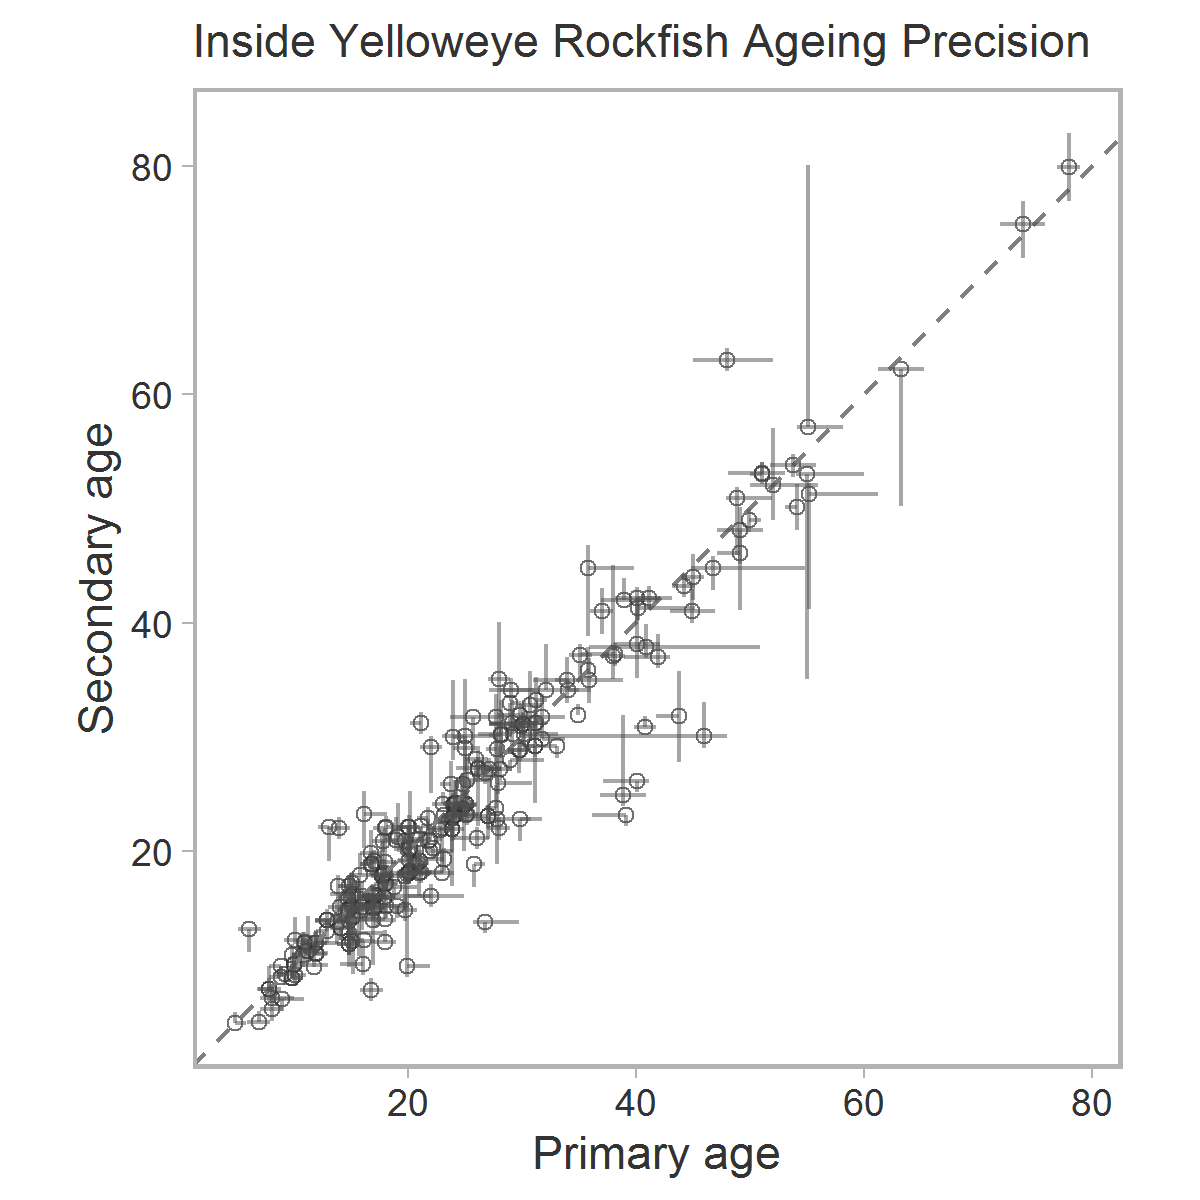
\includegraphics[width=4in]{C:/GitHub/yelloweye-inside/figs/ye-ins-age-precision}}{Figure \ref{fig:age-precision}} 

}

\caption{Ageing precision plot for inside Yelloweye Rockfish. Each dot and cross-hatch represents an individual fish that has been aged twice. The x-axis represents the age and upper and lower ends of the possible age range recorded for the initial (`primary') ageing of the fish. The y-axis represents the equivalent values recorded for the second (`precision') ageing of the fish by a different technician. The dashed diagonal line represents a perfect one-to-one agreement between the two ages. 300 fish have been randomly sampled from all Yelloweye Rockfish precision-aged, and a small amount of random jitter has been added to both axes to reduce overplotting with the same jitter value added to both the x and y axes for a given fish.}\label{fig:age-precision}
\end{figure}

\begin{figure}[htb]

{\centering \pdftooltip{\includegraphics[width=5in]{C:/GitHub/yelloweye-inside/mse/figures/length-freq}}{Figure \ref{fig:length-freq}} 

}

\caption{Length-frequency plot for Inside Yelloweye Rockfish from all available surveys in Area 4B: hard-bottom longline surveys (northern and southern) in inside waters (HBLL INS N/S), hard-bottom longline surveys in outside waters (a small portion of area 4B was included in this survey in 2014 and 2016; HBLL OUT S), and ``OTHER'' surveys including jig surveys in 1985 and 1986 and a bottom trawl survey in 2005. Female fish are shown as coloured bars and male fish are shown behind as light grey bars. The total number of fish measured for a given survey and year are indicated in the top left corner of each panel.}\label{fig:length-freq}
\end{figure}
\begin{figure}[htb]

{\centering \pdftooltip{\includegraphics[width=0.6\textwidth]{C:/GitHub/yelloweye-inside/mse/figures/length-weight}}{Figure \ref{fig:length-weight}} 

}

\caption{Length-weight model fits and plots for inside Yelloweye Rockfish. Female model fits are indicated as solid black lines and male model fits are indicated as dashed grey lines. Text on the panels shows the parameter estimates and open grey circles represent individual fish that the models are fit to. These figures include all survey samples in area 4B.}\label{fig:length-weight}
\end{figure}
\begin{figure}[htb]

{\centering \pdftooltip{\includegraphics[width=0.6\textwidth]{C:/GitHub/yelloweye-inside/mse/figures/vb}}{Figure \ref{fig:length-age}} 

}

\caption{Length-age model fits and plots for inside Yelloweye Rockfish. Female model fit is indicated as a solid black line, male model fit is indicated as a dashed grey line, and combined sex model fit is indicated by a thin black line. Text shows the parameter estimates and open grey circles represent individual fish that the models are fit to. These figures include all survey samples.}\label{fig:length-age}
\end{figure}
\begin{figure}[htb]

{\centering \pdftooltip{\includegraphics[width=0.6\textwidth]{C:/GitHub/yelloweye-inside/mse/figures/mat-ogive-age}}{Figure \ref{fig:percent-maturity}} 

}

\caption{Age-at-maturity ogive plots for inside Yelloweye Rockfish. The solid black lines represent fits to the female fish and the dashed grey lines represent fits to the male fish. The vertical lines indicate the estimated age at 50\% maturity. Text on the panels indicates the estimated age at 5, 50 and 95\% maturity for females (F) and males (M). Short rug lines along the top and bottom represent up to 1500 randomly chosen individual fish with a small amount of random jittering to help differentiate individual fish.}\label{fig:percent-maturity}
\end{figure}

\begin{figure}[htb]

{\centering \pdftooltip{\includegraphics[width=0.6\textwidth]{C:/GitHub/yelloweye-inside/mse/figures/mat-prop}}{Figure \ref{fig:prop-mature}} 

}

\caption{Predicted and observed proportions mature-at-age for inside Yelloweye Rockfish.}\label{fig:prop-mature}
\end{figure}

\begin{figure}[htb]

{\centering \pdftooltip{\includegraphics[width=0.6\textwidth]{C:/GitHub/yelloweye-inside/mse/figures/mat-months}}{Figure \ref{fig:mat-months}} 

}

\caption{Maturity-frequency-by-month plot for inside Yelloweye Rockfish. The area of each circle corresponds to the number of fish specimens in a given maturity category for the given month. Female fish are indicated by black circles and male fish are indicated by light grey circles behind. The total number of fish specimens for each month are indicated by the numbers at the top of the plot.}\label{fig:mat-months}
\end{figure}
\clearpage

\hypertarget{summary-table-of-biological-data-available}{%
\appsection{SUMMARY TABLE OF BIOLOGICAL DATA AVAILABLE}\label{summary-table-of-biological-data-available}}
\begin{longtable}[]{@{}ccccccc@{}}
\caption{\label{tab:test}Inside Yelloweye Rockfish biological data.}\tabularnewline
\toprule
Year & Specimens & Lengths & Weights & Maturities & Ages & Age specimen collected\tabularnewline
\midrule
\endfirsthead
\toprule
Year & Specimens & Lengths & Weights & Maturities & Ages & Age specimen collected\tabularnewline
\midrule
\endhead
1984 & 2 & 1 & 2 & 1 & 0 & 2\tabularnewline
1985 & 87 & 83 & 83 & 86 & 87 & 87\tabularnewline
1986 & 37 & 37 & 37 & 37 & 28 & 37\tabularnewline
1987 & 5 & 5 & 5 & 5 & 0 & 5\tabularnewline
1988 & 12 & 10 & 10 & 12 & 0 & 12\tabularnewline
1992 & 2 & 2 & 2 & 2 & 0 & 2\tabularnewline
1993 & 1 & 1 & 1 & 1 & 0 & 1\tabularnewline
2003 & 135 & 131 & 130 & 107 & 135 & 135\tabularnewline
2004 & 118 & 117 & 115 & 80 & 118 & 118\tabularnewline
2005 & 146 & 141 & 134 & 124 & 146 & 146\tabularnewline
2007 & 65 & 65 & 64 & 53 & 65 & 65\tabularnewline
2008 & 38 & 37 & 30 & 23 & 32 & 38\tabularnewline
2009 & 10 & 10 & 10 & 10 & 8 & 10\tabularnewline
2010 & 153 & 153 & 153 & 145 & 153 & 153\tabularnewline
2011 & 266 & 264 & 264 & 263 & 264 & 266\tabularnewline
2012 & 171 & 170 & 169 & 144 & 169 & 171\tabularnewline
2013 & 223 & 222 & 223 & 209 & 220 & 223\tabularnewline
2014 & 191 & 191 & 190 & 178 & 159 & 191\tabularnewline
2015 & 236 & 232 & 230 & 219 & 209 & 236\tabularnewline
2016 & 257 & 257 & 257 & 247 & 253 & 257\tabularnewline
2018 & 55 & 55 & 55 & 52 & 55 & 55\tabularnewline
\bottomrule
\end{longtable}
\clearpage


\clearpage

\refstepcounter{chapter}
\label{app:index-data}
\starredchapter{APPENDIX~\thechapter. FISHERY-INDEPENDENT SURVEY DATA}

We conditioned the operating models using indices of abundance from the inside Hard Bottom Longline (HBLL) survey and the Strait of Georgia Dogfish Longline survey. Survey design and modelling of indices for each survey are described here.

\hypertarget{sec:hbll-index-data}{%
\appsection{INSIDE HBLL SURVEY INDEX}\label{sec:hbll-index-data}}

The Inside HBLL survey for the Strait of Georgia management area (4B) has been providing catch-rate indices and associated biological data for inshore rockfish assessment since 2003 (Lochead and Yamanaka \protect\hyperlink{ref-lochead2007}{2007}). The survey has a depth-stratified random design consisting of 2km by 2km survey blocks, and has always taken place on the CCGS Neocaligus vessel. The survey uses size 13/0 snap-type circle hooks and squid bait with a two-hour soak time. Hook-by-hook data, which has been collected since the start of the survey, is electronically collected and stored in a database. For further details on survey design see Lochead and Yamanaka (\protect\hyperlink{ref-lochead2004}{2004}).

The survey area is divided into northern and southern regions (Figure~\ref{fig:map-HBLL-NS}), which are fished in alternating years. The border between the two regions occurs approximately at the northern ends of Pacific Fishery Management Areas (PFMAs) 14 and 15 (Figure~\ref{fig:map-4B}). However, several irregularities have occurred (Figure~\ref{fig:hbll-raw}):


\begin{figure}[htb]

{\centering \pdftooltip{\includegraphics[width=5in]{C:/GitHub/yelloweye-inside/figs/YE_Inside_2019_HBLL_L}}{Figure \ref{fig:map-HBLL-NS}} 

}

\caption{Map of HBLL survey blocks indicating the northern (blue) and southern (green) regions. RCAs (orange blocks) are also shown.}\label{fig:map-HBLL-NS}
\end{figure}
\begin{itemize}

\item
  The survey did not take place in 2006 and 2017.
\item
  The length of the survey has varied annually, and has lead to inconsistencies in the geographic extent surveyed between years.
\item
  Desolation Sound (PFMA 15) is allocated as part of the southern region, but was sampled as part of the northern region in 2003, 2008, and 2019, and not sampled in 2009 and 2018. Catch rates of Yelloweye Rockfish are highest in Desolation Sound (PFMA 15; Figure~\ref{fig:map-4B}). Therefore, we expect the lack of sampling in 2009 and 2018 to have an effect on survey estimates from the southern survey.
\item
  The full southern survey was not completed in 2009 where only 38 blocks were fished in the southern Strait of Georgia, and only between Nanaimo and Victoria. This is in contrast to normal years when approximately 70 blocks are fished as far north as Campbell River. Catch rates of most rockfish species caught on this survey tend to decline from the north to the south, so this could also have a major effect on the survey index in that year.
\end{itemize}
We applied a geostatistical spatiotemporal model to standardize of the HBLL index (e.g., Shelton et al. \protect\hyperlink{ref-shelton2014}{2014}; Thorson et al. \protect\hyperlink{ref-thorson2015}{2015}; Anderson et al. \protect\hyperlink{ref-anderson2019synopsis}{2019}) to account for the irregular implementation of the survey design (Section~\ref{sec:hbll-spatiotemporal}). We confirmed, via simulation, that this approach can ``stitch'' together the north and south survey regions with relatively little bias (Section~\ref{sec:hbll-sim}).

\hypertarget{sec:hbll-hook-competition}{%
\subsection{Hook competition}\label{sec:hbll-hook-competition}}

A longline index of species abundance may not be proportional to actual abundance under certain conditions. For example, if there is a high degree of competition among species for baited hooks, the actual catch may not accurately reflect the true abundance of less competitive species (Kuriyama et al. \protect\hyperlink{ref-kuriyama2018}{2018}). The Inside HBLL survey catch is mostly comprised of North Pacific Spiny Dogfish (\emph{Squalus suckleyi}; hereafter ``Dogfish''), which are potentially a major hook competitor with rockfishes (Obradovich \protect\hyperlink{ref-obradovich2018}{2018}). As in Yamanaka et al. (\protect\hyperlink{ref-yamanaka2011}{2011}), we applied a hook competition correction, which accounts for the competition between individual fish for the bait on hooks, to the HBLL survey data. To apply the correction, a competition adjustment factor is estimated for each set, in each year. This adjustment factor, \(A_{i,t}\), scales up the observed number of Yelloweye Rockfish caught, \(N_{i,t}\), for each set \(i\) in each year \(t\) to give the expected number of fish caught after accounting for competition, \(N_{i,t}^{(0)}\):
\begin{equation}
N_{i,t}^{(0)} = A_{i,t} N_{i,t}.
\label{eq:Nit}
\end{equation}
The adjustment factor depends on the proportion of observed hooks that are returned with bait still on them, \(P_{i,t}\) (Figure~\ref{fig:hbll-baited}):
\begin{equation}
A_{i,t} = - \frac{ \log P_{i,t}}{1 - P_{i,t}}.
\label{eq:hbll-hook-adjustment}
\end{equation}
As \(P_{i,t} \rightarrow 0\), \(A_{i,t} \rightarrow \infty\), so that the expected number \(N_{i,t}^{(0)} \rightarrow \infty\). Therefore, in cases where zero hooks were returned with bait, we set the number of baited hooks to one. See Anderson et al. (\protect\hyperlink{ref-anderson2019synopsis}{2019}) (their Appendix G, Section G.5) for further details on the hook competition correction. We passed the hook-competition-adjusted data (Figure~\ref{fig:hbll-hook-adjustment}) to the spatiotemporal model to develop the index of abundance.

\hypertarget{sec:hbll-spatiotemporal}{%
\subsection{Spatiotemporal HBLL index standardization}\label{sec:hbll-spatiotemporal}}

We fit a geostatistical spatiotemporal index-standardization model:
\begin{align}
  y_{s,t} &\sim \mathrm{NegBin}\left(\mu_{s,t}, \phi \right),\\
  \mu_{s,t} &= \exp \left( \bm{X}_{s,t} O_{s,t} + \bm{\beta} + \omega_s + \epsilon_{s,t} \right),
\label{eq:hbll-model}
\end{align}
where NegBin refers to the negative binomial distribution (the NB2 parameterization (Hilbe \protect\hyperlink{ref-hilbe2011}{2011}) where the variance scales quadratically with the mean), \(\phi\) represents the dispersion parameter, \(y_{s,t}\) and \(\mu_{s,t}\) refers to the observed and expected value, respectively, at spatial point \(s\) and time \(t\), \(\phi\) refers to the dispersion parameter, \(\bm{X}\) refers to a design matrix, and \(\beta\) refers to a vector of estimated coefficients (an independent mean for each year). The symbol \(O_{s,t}\) represents an ``offset'' for the number of hooks and the hook-competition-adjustment factor. Specifically, it was represented as \(\log \left(S_{i,t} / A_{i,t} \right)\), where \(S_{i,t}\) represents the area ``swept'' by the set. We calculated of the area swept based on the number of hooks (\(N^\textrm{hooks}_{i,t}\)) in set \(i\) and year \(t\) as:
\begin{equation}
N^\textrm{hooks}_{i,t} \cdot 0.0024384 \cdot 0.009144 \cdot 1000.
\end{equation}
The value 0.002438 corresponds to the spacing between hooks (8 ft) in kms, 0.009144 to an assumed 30 ft area swept around the set that fish are catchable (in kms), and 1000 scales the area swept from km to m. Note that the 30 ft assumption only serves to scale the density up or down in all years and ultimately affects the survey-catchability estimate but will not influence the shape of the index timeseries.

We assumed that the spatial random effects (\(\omega_s\)) were drawn from a multivariate normal distribution with a covariance matrix \(\bm{\Sigma}_\omega\):
\begin{equation}
\bm{\omega} \sim \mathrm{MVNormal} \left( \bm{0}, \bm{\Sigma}_\omega \right).
\end{equation}
We constrained the spatial random effects to follow a \mbox{Mat\'ern} covariance function, which defines the rate with which spatial correlation decays with distance. The \mbox{Mat\'ern} function describes the covariance \(\Phi_\omega \left( s_j, s_k \right)\) between spatial locations \(s_j\) and \(s_k\) as:
\begin{equation}
\Phi_\omega\left( s_j,s_k \right) = \tau_\omega^2/\Gamma(\nu)2^{\nu - 1}
    (\kappa d_{jk})^\nu K_\nu \left( \kappa d_{jk} \right),
\end{equation}
where \(\tau_\omega^2\) represents the spatial variance, \(\Gamma\) represents the Gamma function, \(K_\nu\) represents the Bessel function, \(d_{jk}\) represents the Euclidean distance between locations \(s_j\) and \(s_k\), and \(\kappa\) represents a scaling parameter that is estimated (e.g., Lindgren et al. \protect\hyperlink{ref-lindgren2011}{2011}). The parameter \(\nu\) controls the smoothness of the covariance function. We set \(\nu = 1\), which lets us take advantage of the Stochastic Partial Differential Equation (SPDE) approximation to Gaussian Markov Random Fields (GMRF) to greatly increase computational efficiency (Lindgren et al. \protect\hyperlink{ref-lindgren2011}{2011}).

We assumed the same structure for the spatiotemporal random effects, with each time slice being given its own independent set of random effects (\(\bm{\epsilon}_t\)) with covariance matrix \(\bm{\Sigma}_{\epsilon,t}\):
\begin{equation}
\bm{\epsilon}_t \sim \mathrm{MVNormal} \left( \bm{0}, \bm{\Sigma}_{\epsilon,t} \right).
\end{equation}
This covariance matrix is also constrained to follow a \mbox{Mat\'ern} covariance function with the same \(\kappa\) but its own \(\tau_\epsilon^2\) (spatial variance):
\begin{equation}
\Phi_\epsilon\left( s_j,s_k \right) = \tau_\epsilon^2/\Gamma(\nu)2^{\nu - 1}
    (\kappa d_{jk})^\nu K_\nu \left( \kappa d_{jk} \right).
\end{equation}
Although we have described the \mbox{Mat\'ern} functions above using the simple isometric form for simplicity (spatial correlation is the same in all directions), we actually allowed for anisotropy in the spatial and spatiotemporal correlation (e.g., Thorson et al. \protect\hyperlink{ref-thorson2015}{2015}).

The spatial random effects accounted for spatial factors that were constant across time, for example, depth and substrate type. The spatiotemporal random effects accounted for factors that varied spatially from year-to-year, such as bottom temperature, water circulation patterns, species interactions, and species movement. As sensitivity analyses, we included alternate versions of our models that: (1) also accounted for depth; and (2) did not account for hook competition.

We fit our model with the sdmTMB R package (Anderson et al. \protect\hyperlink{ref-sdmtmb}{2020}\protect\hyperlink{ref-sdmtmb}{a}) and TMB (Kristensen et al. \protect\hyperlink{ref-tmb}{2016}) using a ``mesh'' with 400 predictive-process ``knots'' generated by INLA (Lindgren et al. \protect\hyperlink{ref-lindgren2011}{2011}; Rue et al. \protect\hyperlink{ref-rue2016}{2016}) with locations determined by a K-means clustering algorithm (Figure~\ref{fig:hbll-spde}). We estimated the fixed effects via maximum likelihood with the random effects set to the values that maximized the joint likelihood conditional on the estimated value of fixed effects. We checked that the model fits were consistent with convergence by checking that the maximum gradient across all estimated coefficients was \textless{} 0.001 and that the covariance matrix was positive-definite.

We projected predictions from the model to the full survey domain (Figure~\ref{fig:hbll-area-grid}) using the covariance projection matrix and the bilinear interpolation mesh provided by INLA (Lindgren et al. \protect\hyperlink{ref-lindgren2011}{2011}; Rue et al. \protect\hyperlink{ref-rue2016}{2016}) (Figures~\ref{fig:hbll-spde} and~\ref{fig:hbll-predicted-spacetime}). In terms of the model components, the spatial random effects were, by definition, constant across years (Figure~\ref{fig:hbll-spatial-re}), and the spatiotemporal random effects varied across years (Figure~\ref{fig:hbll-spatiotemporal-re}).

We then calculated expected biomass \(B_t\) in year \(t\) as:
\begin{equation}
B_t = \sum_{j = 1}^{n_j}
  w_j \cdot \exp \left( \bm{X}_{j,t} \bm{\beta} + \bar{\bm{O}} + \omega_j + \epsilon_{j,t} \right),
\end{equation}
where \(j\) references a grid cell within the survey domain, \(w_j\) represents the area of that grid cell (Figure~\ref{fig:hbll-area-grid}), and \(\bar{\bm{O}}\) represents the mean offset value. In other words, we summed the predicted biomass across all grid cells within the survey domain for each year. We generated standard errors on the annual estimates of log biomass via the generalized delta method as implemented in TMB (Kristensen et al. \protect\hyperlink{ref-tmb}{2016}).

The resulting standardized population index accounts for the irregular sampling of the survey domain and hook competition and ``stitches'' the northern and southern regions into a single population index (Figure~\ref{fig:hbll-index}). The inclusion of depth or the exclusion of the hook competition adjustments had relatively minor effects on the population index (Figure~\ref{fig:hbll-index}). The model was also able to ``fill in'' what the index might hypothetically look like for the northern and southern regions independently (Figure~\ref{fig:hbll-index}). Note that this statistical interpolation cannot account for one-off events in the unobserved region, such as an abnormally high abundance only in the northern region in a year when the southern region was surveyed.

\hypertarget{sec:hbll-sim}{%
\subsection{Simulation-testing survey ``stitching'' via spatiotemporal models}\label{sec:hbll-sim}}

We undertook a basic simulation analysis to test that our approach of ``stitching'' northern and southern regions into a single survey domain was reasonable from a statistical perspective. We generated a system that roughly matches the HBLL survey data we worked with in this document:
\begin{itemize}

\item
  10 years of observations
\item
  100 possible spatial observation locations \(s_j\) and \(s_k\) drawn from a Uniform(0, 1) distribution each year.
\item
  A marginal SD(\(\omega_s\)) = 2.2
\item
  A marginal SD(\(\epsilon_{s,t}\)) = 0.3
\item
  A \mbox{Mat\'ern} parameter \(\kappa = 0.1\)
\item
  Annual means drawn from a Lognormal(0.1, 0.2) distribution
\item
  A Poisson observation process (for simplicity vs.~a negative binomial)
\end{itemize}
We simulated the underlying true mean abundance on a complete {[}0, 1{]} grid with 25 x 25 evenly sized grid cells. We then discarded the northern and southern regions (above or below 0.5) in alternating years, to render approximately 50 observations per year, and attempted to fit the same form of spatiotemporal model as the one used for the HBLL index standardization (Figure~\ref{fig:stich-sim-pred}).

Despite the model only observing alternating northern and southern regions, the model was able to reconstruct the unobserved missing portions based on the estimated spatial correlation, and to a lesser extent, the estimated spatiotemporal correlation (Figure~\ref{fig:stich-sim-pred}). By projecting the model predictions onto a grid over the full area of the simulated square, our model was able to produce an index that was similar to the true index (Figure~\ref{fig:stich-sim-index}). If we instead naively generated the index using an approach to mimic a design-based approach (by summing the observed abundances each year and scaling it to the same geometric mean for visualization purposes), the resulting index does not reflect the true index trend in many years (Figure~\ref{fig:stich-sim-index}).

Through experimentation (not shown) we found that the stitching was most accurate at recapturing the true index if the magnitude of spatial correlation deviations (\(\omega_s\)) was much larger than the magnitude of spatiotemporal correlation deviations (\(\epsilon_{s,t}\)). This is the case in our HBLL model, where the marginal standard deviation of \(\omega_s\) was approximately six times larger than the marginal standard deviation of \(\epsilon_{s,t}\). The stitching was most needed when there was a north to south gradient in abundance, as seems evident for Yelloweye Rockfish.
\begin{figure}[htb]

{\centering \pdftooltip{\includegraphics[width=\textwidth]{C:/GitHub/yelloweye-inside/figs/hbll-joint-raw-data}}{Figure \ref{fig:hbll-raw}} 

}

\caption{Inside HBLL survey observations of Yelloweye Rockfish. Gray background shading indicates the northern and southern survey areas. The area of the circles represents the number of fish caught per hook after accounting for hook competition.}\label{fig:hbll-raw}
\end{figure}
\begin{figure}[htb]

{\centering \pdftooltip{\includegraphics[width=5in]{C:/GitHub/yelloweye-inside/figs/hbll-area-in-water}}{Figure \ref{fig:hbll-area-grid}} 

}

\caption{Area per survey grid cell that is in water for the inside HBLL survey. The predicted count density for each grid cell is scaled up to the full survey domain based on these areas.}\label{fig:hbll-area-grid}
\end{figure}
\begin{figure}[htb]

{\centering \pdftooltip{\includegraphics[width=\textwidth]{C:/GitHub/yelloweye-inside/figs/hbll-joint-baited}}{Figure \ref{fig:hbll-baited}} 

}

\caption{Proportion baited hooks returned for the inside HBLL survey. Note the substantial difference between the northern and southern areas and the change in the north between 2003--2007 and subsequent years.}\label{fig:hbll-baited}
\end{figure}
\begin{figure}[htb]

{\centering \pdftooltip{\includegraphics[width=\textwidth]{C:/GitHub/yelloweye-inside/figs/hbll-joint-hook-adjust}}{Figure \ref{fig:hbll-hook-adjustment}} 

}

\caption{Hook adjustment factor for the inside HBLL survey accounting for the number of hooks and the number of returned baited hooks.}\label{fig:hbll-hook-adjustment}
\end{figure}
\begin{figure}[htb]

{\centering \pdftooltip{\includegraphics[width=0.6\textwidth]{C:/GitHub/yelloweye-inside/figs/hbll-joint-spde}}{Figure \ref{fig:hbll-spde}} 

}

\caption{Stochastic Partial Differential Equation (SPDE) mesh for the HBLL. The open grey circles in the background (often hidden) represent the locations of the observed data and the red dots represent the "knots". The lines show the triangularization mesh used in the SPDE approximation and bilinear interpolation. A greater number of knots will increase the accuracy of the approximation at the expense of computational time.}\label{fig:hbll-spde}
\end{figure}
\begin{figure}[htb]

{\centering \pdftooltip{\includegraphics[width=\textwidth]{C:/GitHub/yelloweye-inside/figs/hbll-joint-prediction-log}}{Figure \ref{fig:hbll-predicted-spacetime}} 

}

\caption{Predicted relative density in space and time for the inside HBLL survey. Observed (hook-adjusted) counts are illustrated with circles. Predictions are illustrated with colour shading.}\label{fig:hbll-predicted-spacetime}
\end{figure}
\begin{figure}[htb]

{\centering \pdftooltip{\includegraphics[width=4.2in]{C:/GitHub/yelloweye-inside/figs/hbll-joint-omega}}{Figure \ref{fig:hbll-spatial-re}} 

}

\caption{The spatial random effects. These are consistent spatially correlated differences in expected abundance through time. The values are shown in link (log) space.}\label{fig:hbll-spatial-re}
\end{figure}
\begin{figure}[htb]

{\centering \pdftooltip{\includegraphics[width=\textwidth]{C:/GitHub/yelloweye-inside/figs/hbll-joint-epsilon}}{Figure \ref{fig:hbll-spatiotemporal-re}} 

}

\caption{The spatiotemporal random effects. These are spatially correlated deviations that change through time. Note the reversion to the mean in area-year combinations without sampling data. Note the difference in magnitude between the spatial random effects (previous figure) and these spatiotemporal random effects.}\label{fig:hbll-spatiotemporal-re}
\end{figure}
\begin{figure}[htb]

{\centering \pdftooltip{\includegraphics[width=4in]{C:/GitHub/yelloweye-inside/figs/hbll-index-components-eps-depth2}}{Figure \ref{fig:hbll-index}} 

}

\caption{The joint relative abundance index. Top panel shows the joint prediction from the spatial temporal model. Included are three versions: (1) random effects and annual means only, (2) adding a depth covariate, and (3) removing the hook adjustment factor. The middle and bottom panels show the joint predictions for the northern and southern areas. All shaded regions represent 95\% confidence intervals. The joint index timeseries in the top panel have been scaled to have the same geometric mean as the main ``HBLL INS'' index for visualization purposes. Dashed vertical lines indicate years with surveys (mostly) in the southern area.}\label{fig:hbll-index}
\end{figure}
\clearpage
\begin{figure}[htb]

{\centering \pdftooltip{\includegraphics[width=\textwidth]{C:/GitHub/yelloweye-inside/figs/geostatistical-sim-predicted}}{Figure \ref{fig:stich-sim-pred}} 

}

\caption{Simulation testing the relative abundance index calculation with alternating north and south observations. (A) The true simulated (mean) abundance in space and time. (B) The observed (dots) and estimated (colour) counts in space and time from the geostatistical model. The observations occur in north and south regions in alternating years and are ``blind'' to the missing region. Notice how the spatial temporal model is able to predict what the abundance should be in the ``blind'' region based on the consistent spatial correlation pattern (and to a lesser degree the spatiotemporal correlation pattern).}\label{fig:stich-sim-pred}
\end{figure}
\clearpage
\begin{figure}[htb]

{\centering \pdftooltip{\includegraphics[width=5in]{C:/GitHub/yelloweye-inside/figs/geostatistical-sim-stitched-index}}{Figure \ref{fig:stich-sim-index}} 

}

\caption{Simulation testing the relative abundance index calculation with alternating north and south observations. The solid red line represents the true simulated abundance through time. The dashed and dotted green line represents a ``naive'' design-based estimate, which is calculated here by calculating the abundance with just the observed north or south counts in each year. The dashed blue line represents a geostatistical standardized index that attempts to account for the north-south biennial observations. The shaded blue region represents the modelled 95\% confidence interval.}\label{fig:stich-sim-index}
\end{figure}
\clearpage

\hypertarget{sec:dogfish-index-data}{%
\appsection{DOGFISH SURVEY INDEX}\label{sec:dogfish-index-data}}

The Dogfish survey samples nine locations in the Strait of Georgia that were historically fished by the commercial Dogfish fishery (King et al. \protect\hyperlink{ref-king2012}{2012}). The survey began in 1986 and sampling has occurred in 1989, 2005, 2011, 2014, and 2019. The survey is a depth-stratified longline survey that uses snap on gear with 300 size 14/0circle hooks baited with Pacific Herring and a two-hour soak time. A more detailed description of survey methods is provided in King et al. (\protect\hyperlink{ref-king2012}{2012}). For most of the time series, set-by-set catch of rockfish has been recorded. Beginning in 2019, hook-by-hook data for all captured species were collected on board, along with biological data for rockfish. We use a spatiotemporal model to estimate the density of Yelloweye Rockfish per km\textsuperscript{2}. We calculated the area swept by multiplying the number of hooks deployed by the estimated distance between hooks (8 ft spacing) and the estimated width swept (the length of two gagnions).

The Dogfish survey is not designed to index rockfish, so there are several important differences between the inside HBLL and Dogfish survey designs. Perhaps the most significant difference is that the HBLL specifically targets habitats suitable for rockfish (i.e.~hard bottom), whereas the Dogfish survey visits sites that were important in the commercial fishery that have mainly soft sediment bottoms. The Dogfish survey also uses slightly larger circle hooks than the HBLL survey (14/0 vs.~13/0); herring bait instead of squid; fishes 300 hooks per set instead of 225; and the hooks are spaced 1.8m apart instead of 2.4m. We use the Dogfish survey in this analysis because it provides the longest time series of fishery independent data for inside Yelloweye Rockfish and because it was used in the previous assessment in 2011.

\hypertarget{sec:dog-hook-comparison}{%
\subsection{Hook comparison}\label{sec:dog-hook-comparison}}

The survey fished with J hooks originally and then changed to circle hooks in 2005. In 2004, McFarlane et al. (\protect\hyperlink{ref-mcfarlane2005}{2005}) undertook a calibration study to assess the potential for a change in catch rates due to the change in hook type. However, the study compared catch rates for Dogfish only, and the hook change likely affected catchability for Yelloweye Rockfish differently than for Dogfish. The previous assessment attempted to deal with this by estimating a catchability ratio, using data for all rockfish, to scale the catch in the 1980s (Yamanaka et al. \protect\hyperlink{ref-yamanaka2011}{2011}). It is not clear from their description how this catchability ratio was estimated. The previous assessment was quite sensitive to the resulting Dogfish index (because of the large decline from the 1980s), and that decline was largely dependent on the hook ratio.

In the hook comparison study, 23 sets used circle hooks and 23 sets used J hooks. On these experimental sets, 5 Yelloweye Rockfish were caught on J hooks and 27 were caught on circle hooks Table~\ref{tab:dogfish-hook-comparison}. Although this represents a relatively small sample size of fish for estimating a hook correction factor for Yelloweye Rockfish, by simultaneously estimating the correction factor while standardizing the population index using a geostatistical model, we were able to incorporate uncertainty in the correction factor into the resulting index standard errors (Section~\ref{sec:dog-index-model}). Nonetheless, it is important to note that this correction factor is based on a limited number of sets. It is driven largely by five sets with one or two more Yelloweye Rockfish caught by circle hooks than J hooks and two sets with 12 and four Yelloweye Rockfish caught by circle hooks vs.~zero by J hooks (Table~\ref{tab:dogfish-hook-comparison}).

\clearpage
\begin{longtable}[]{@{}rrr@{}}
\caption{\label{tab:dogfish-hook-comparison}Number of Yelloweye Rockfish caught in J-hook/circle-hook experiment in 2004.}\tabularnewline
\toprule
Set & J-hook & Circle hook\tabularnewline
\midrule
\endfirsthead
\toprule
Set & J-hook & Circle hook\tabularnewline
\midrule
\endhead
1 & 0 & 0\tabularnewline
2 & 0 & 1\tabularnewline
3 & 0 & 0\tabularnewline
4 & 0 & 0\tabularnewline
5 & 0 & 2\tabularnewline
6 & 0 & 0\tabularnewline
7 & 1 & 1\tabularnewline
8 & 0 & 0\tabularnewline
9 & 1 & 0\tabularnewline
10 & 0 & 0\tabularnewline
11 & 0 & 12\tabularnewline
12 & 0 & 0\tabularnewline
13 & 0 & 2\tabularnewline
14 & 0 & 0\tabularnewline
15 & 0 & 0\tabularnewline
16 & 0 & 0\tabularnewline
17 & 0 & 1\tabularnewline
18 & 0 & 4\tabularnewline
19 & 0 & 0\tabularnewline
20 & 0 & 0\tabularnewline
21 & 0 & 0\tabularnewline
22 & 0 & 0\tabularnewline
23 & 3 & 4\tabularnewline
\bottomrule
\end{longtable}
\hypertarget{sec:dog-depth}{%
\subsection{Depth}\label{sec:dog-depth}}

In addition to the survey not being designed for rockfishes, and the change in gear type, the shallower depth stratum was dropped in 2004 and later surveys. This was done to purposely try to avoid catching rockfish (because of conservation concerns). While depth is not explicitly included in the spatiotemporal model, the spatial random effects should absorb much of the variation driven by depth while also accounting for other spatially varying effects.

\hypertarget{sec:dog-hook-competition}{%
\subsection{Hook competition}\label{sec:dog-hook-competition}}

The previous inside Yelloweye Rockfish assessment indicates they used an exponential hook competition model on the Dogfish Survey data in 2011. However, there are no data on the number of baited and empty hooks available for the Dogfish Survey prior to 2019 and it is unclear how the previous assessment accounted for this. Therefore, we did not apply an explicit hook competition model in the present analysis. However, to partially account for hook competition, we included the number of Dogfish caught (log transformed so as to have a multiplicative effect on observed account) as a covariate in the model.

\hypertarget{sec:dog-index-model}{%
\subsection{Spatiotemporal Dogfish survey index standardization}\label{sec:dog-index-model}}

We used a similar geostatistical model to that described for the HBLL survey (Section~\ref{sec:hbll-spatiotemporal}) with the addition of Dogfish and hook-type covariates. We included the log Dogfish count and hook-type in the model matrix \(\bm{X}_{s,t}\):
\begin{align}
  y_{s,t} &\sim \mathrm{NegBin}(\mu_{s,t}, \phi),\\
  \mu_{s,t} &= \exp \left( \bm{X}_{s,t} \bm{\beta} + O_{s,t} + \omega_s + \epsilon_{s,t} \right),
\label{eq:dogfish-model}
\end{align}
with symbols defined as in Equation~\ref{eq:hbll-model}. Hook-type is an identifier for J-hook vs.~circle-hook. The offset represents the log(area swept), as previously defined. We fit our model with sdmTMB (Anderson et al. \protect\hyperlink{ref-sdmtmb}{2020}\protect\hyperlink{ref-sdmtmb}{a}) as described above with 300 knots.

In our projection of the model predictions onto the survey grid to calculate the standardized relative abundance:
\begin{equation}
B_t = \sum_{j = 1}^{n_j}
  w_j \cdot \exp \left( \bm{X}_{j,t} \bm{\beta} + \bar{\bm{O}} + \omega_j + \epsilon_{j,t} \right),
\label{eq:dog-prediction}
\end{equation}
with symbols defined as above, we could predict for a J-hook or a circle hook. Choosing one or the other would place more of the uncertainty in the years with one or the other since the other effect's uncertainty would be incorporated in only some years. As a compromise, we chose to predict for an average hook type across the data set to distribute this hook-type uncertainty across the timeseries. In practice, this meant coding circle hooks as -0.57 and J hooks as 0.43 in the model-fitting matrix \(\bm{X}_{s,t}\) and setting the equivalent predictor in the prediction model matrix to 0.

We estimated that J hooks caught 7.7 times more Yelloweye Rockfish than circle-hooks, all else being equal, but with considerable uncertainty (95\% confidence interval (CI): 1.6 -- 37.1). We estimated the log Dogfish effect to be -0.31 (95\% CI: -0.59 -- -0.03). This means that we can expect to catch, on average, about 3.1\% (95\% CI: 0.3\% -- 5.9\%) fewer Yelloweye Rockfish for every 10\% additional Dogfish also caught on the same set, presumably due to hook competition.

In Equation~\ref{eq:dog-prediction}, we set up the prediction grid cells, indexed by \(j\), by overlaying a 500 m x 500 m grid on the survey-domain. Because the Dogfish survey uses fixed stations rather than a randomly sampled grid, rectangles were manually drawn around all of the historically fished longline sets in order to delineate the area sampled (Figure~\ref{fig:dog-raw}). We calculated the grid cell areas (\(w_j\)) after removing a portion of the fine-scale grid cells that overlapped land. We set up the design matrix \(\bm{X}_{j,t}\) to predict for a mean Dogfish count and a mean area-swept offset.

The resulting projection of the model onto the fine-scale grid is shown in Figure~\ref{fig:dog-prediction} along with the modelled spatial (Figure~\ref{fig:dog-spatial}) and spatiotemporal (Figure~\ref{fig:dog-spatiotemporal}) random-effect values. The standardized index for Yelloweye Rockfish for an average hook type indicates a decline in relative abundance from the 1980s to the next survey in 2004, but with considerable uncertainty (Figure~\ref{fig:dog-standardized-index}). The index remained relatively stationary from 2004 until 2014 with a slight increase in the mean from 2014 to 2019, but again with considerable uncertainty (Figure~\ref{fig:dog-standardized-index}).

\clearpage
\begin{figure}[htb]

{\centering \pdftooltip{\includegraphics[width=\textwidth]{C:/GitHub/yelloweye-inside/figs/dogfish-yelloweye-per-area-data}}{Figure \ref{fig:dog-raw}} 

}

\caption{Yelloweye Rockfish caught per area swept by hooks in the Dogfish Survey. The values are shown as area of circles. Grey rectangles illustrate the assumed survey domain.}\label{fig:dog-raw}
\end{figure}
\begin{figure}[htb]

{\centering \pdftooltip{\includegraphics[width=\textwidth]{C:/GitHub/yelloweye-inside/figs/dogfish-prediction-log}}{Figure \ref{fig:dog-prediction}} 

}

\caption{Predicted Yelloweye Rockfish relative abundance (colour). The colour scale is log transformed. Circles represent the same observed data as in the previous figure.}\label{fig:dog-prediction}
\end{figure}
\begin{figure}[htb]

{\centering \pdftooltip{\includegraphics[width=4.2in]{C:/GitHub/yelloweye-inside/figs/dogfish-omega}}{Figure \ref{fig:dog-spatial}} 

}

\caption{Spatial random effects from the spatiotemporal model shown in log space. This represents consistent spatial correlation through time.}\label{fig:dog-spatial}
\end{figure}
\begin{figure}[htb]

{\centering \pdftooltip{\includegraphics[width=\textwidth]{C:/GitHub/yelloweye-inside/figs/dogfish-epsilon}}{Figure \ref{fig:dog-spatiotemporal}} 

}

\caption{Spatiotemporal random effects from the spatiotemporal model shown in log space. These panels represent spatial correlation that varies through time.}\label{fig:dog-spatiotemporal}
\end{figure}
\begin{figure}[htb]

{\centering \pdftooltip{\includegraphics[width=5in]{C:/GitHub/yelloweye-inside/figs/dogfish-index-estimated-hook}}{Figure \ref{fig:dog-standardized-index}} 

}

\caption{The resulting standardized Yelloweye Rockfish relative abundance index. Dots represent mean estimates and line segments represent 95\% confidence intervals. The dashed vertical line represents the year of the hook experiment and the switch from J hooks to circle hooks.}\label{fig:dog-standardized-index}
\end{figure}
\clearpage


\clearpage

\refstepcounter{chapter}
\label{app:catch-data}
\starredchapter{APPENDIX~\thechapter. CATCH DATA}

Inside Yelloweye Rockfish is targeted in hook and line commercial fisheries, Food Social and Ceremonial (FSC) fisheries, and recreational fisheries. Management of Inside Yelloweye Rockfish fisheries began in 1986, with the introduction of the ``ZN'' category commercial licence and daily bag limits for recreational fishermen. A chronology of management changes for commercial and recreational fisheries is shown in Tables~\ref{tab:comm-mgt-changes} and~\ref{tab:rec-mgt-changes}.

\hypertarget{sec:com-catch-data}{%
\appsection{COMMERCIAL CATCH DATA}\label{sec:com-catch-data}}

Rockfish catch data can be grouped into three time periods: historic (1918-1950), early electronic (1951--2005), and modern (2006 onwards). There are two major sources of uncertainty in the historical and early electronic periods for Inside Yelloweye Rockfish. The first uncertainty is that rockfish catch, other than Pacific Ocean Perch (\emph{Sebastes alutus}), was reported as an aggregate (other rockfish, ORF) in the historic period. To reconstruct historical catches an algorithm was developed by DFO authors (Haigh and Yamanaka \protect\hyperlink{ref-haigh2011}{2011}). The reconstruction algorithm applies a ratio calculated from a period with credible landings data from the hook and line dockside monitoring program (1997--2005) to generate a time series of catch by species, year, fishery sector, and management area (Haigh and Yamanaka \protect\hyperlink{ref-haigh2011}{2011}). ``Credible'' landings data are taken from reference years where catch knowledge was considered high quality and stable, beginning in 1997 with the start of observer trawl coverage and the individual vessel quota system (Haigh and Yamanaka \protect\hyperlink{ref-haigh2011}{2011}).

The second major source of uncertainty is the magnitude of unreported catch that was released or discarded at sea, prior to the introduction of 100\% observer coverage in 2006. The catch reconstruction of Haigh and Yamanaka (\protect\hyperlink{ref-haigh2011}{2011}) assumes no discarding prior to 1986, when the ZN licence was instituted. Prior to that it is assumed all rockfish were kept. Discards are assumed to be fully reported in DFO databases since 2006 and the introduction of 100\% observer coverage. Non-retained Yelloweye Rockfish catch (releases or discards) was estimated for each fishery using the ratio of Yelloweye Rockfish discarded by a fishery to fishery-specific landed targets using data from 2000--2004 hook and line observer logs. The estimated historical unreported catch was then incorporated into the catch reconstruction, giving a final annual total.

The commercial catch time series used in this analysis (Figure~\ref{fig:commcatch2} and Table~\ref{tab:commcatch}) differs from the one previously reported in 2009, for several reasons. Ongoing quality control and updates to the groundfish catch database resulted in minor differences in the data over time (Maria Surry, DFO, Pacific Biological Station, pers. comm., March 9, 2020). As well, an earlier version of the catch reconstruction algorithm was used to develop the time series for the previous stock assessment, as the final version had not yet been published. Further refinements to the reconstruction algorithm resulted in significant changes to the estimated historical catch in some years (Norm Olsen, DFO, Pacific Biological Station, pers. comm., March 9,2020).

The reconstruction algorithm could have been applied to all years in the time series until to 2005 (after which, full at-sea and dockside monitoring came into effect). However, for this analysis we used the reconstructed catch data from 1918--1985, and switched to the nominal catch data in 1986. The nominal catch from 1986--2005 was then doubled,to be consistent with the previous assessment (Yamanaka et al. \protect\hyperlink{ref-yamanaka2011}{2011}). We made the choice to double the nominal catch rather than the reconstructed catch because, prior to the previous assessment, advice from industry representatives indicated they did not have confidence in the catch reconstruction between 1986 and 2005, and that the scale of unreported catch was probably equal to landed catch (DFO \protect\hyperlink{ref-dfo2012b}{2012}\protect\hyperlink{ref-dfo2012b}{b}). As a result of this advice, the catch for these years was doubled (Yamanaka et al. \protect\hyperlink{ref-yamanaka2011}{2011}). However, because discards are estimated as part of the catch reconstruction algorithm, in the current analysis we doubled the nominal catch for the period 1986--2005 (rather than the reconstructed catch), to avoid double counting of discards. As a sensitivity check, we explore one OM scenario where the 1986--2005 commercial catches were not doubled (the ``Low catch'' Scenario (2), Section~\ref{sec:approach3-reference2}).
\begin{figure}[htb]

{\centering \pdftooltip{\includegraphics[width=0.8\textwidth]{knitr-figs-pdf/commcatch2-1}}{Figure \ref{fig:commcatch2}} 

}

\caption{Commercial catch by sector for Inside Yelloweye Rockfish. This figure contains reconstructed (1918--1985) and nominal (1986--2019) catch estimates in tonnes.}\label{fig:commcatch2}
\end{figure}
\clearpage
\begin{longtable}[t]{>{\raggedleft\arraybackslash}p{1.0cm}>{\raggedleft\arraybackslash}p{2cm}>{\raggedleft\arraybackslash}p{2cm}>{\raggedleft\arraybackslash}p{2cm}>{\raggedleft\arraybackslash}p{2cm}>{\raggedleft\arraybackslash}p{2cm}}
\caption{\label{tab:commcatch}Commercial catch by sector for Inside Yelloweye Rockfish. The table contains reconstructed (1918--1985) and nominal (1986--2019) catch estimates in tonnes. Although nominal catch is shown, total catch for each year between 1986-2005 was doubled in all OMs except the 'Low Catch' scenario. This was done for consistency with the previous stock assessment in 2012.}\\
\toprule
\textbf{Year} & \textbf{Trawl} & \textbf{Halibut} & \textbf{Dogfish and Lingcod} & \textbf{Hook and Line Rockfish} & \textbf{Total}\\
\midrule
1918 & 0.00 & 3.40 & 4.90 & 8.80 & 17.10\\
1919 & 0.00 & 8.50 & 12.00 & 22.00 & 42.50\\
1920 & 0.00 & 4.30 & 6.00 & 11.00 & 21.30\\
1921 & 0.00 & 3.70 & 5.20 & 9.50 & 18.40\\
1922 & 0.00 & 4.60 & 6.50 & 12.00 & 23.10\\
1923 & 0.00 & 4.50 & 6.30 & 11.00 & 21.80\\
1924 & 0.00 & 5.10 & 7.20 & 13.00 & 25.30\\
1925 & 0.00 & 4.40 & 6.20 & 11.00 & 21.60\\
1926 & 0.00 & 5.00 & 7.10 & 13.00 & 25.10\\
1927 & 0.00 & 5.00 & 7.10 & 13.00 & 25.10\\
1928 & 0.00 & 5.10 & 7.30 & 13.00 & 25.40\\
1929 & 0.00 & 6.70 & 9.50 & 17.00 & 33.20\\
1930 & 0.00 & 6.00 & 8.60 & 16.00 & 30.60\\
1931 & 0.00 & 4.00 & 5.60 & 10.00 & 19.60\\
1932 & 0.00 & 4.50 & 6.40 & 12.00 & 22.90\\
1933 & 0.00 & 2.20 & 3.10 & 5.70 & 11.00\\
1934 & 0.00 & 2.60 & 3.70 & 6.70 & 13.00\\
1935 & 0.00 & 3.30 & 4.70 & 8.60 & 16.60\\
1936 & 0.00 & 3.60 & 5.10 & 9.30 & 18.00\\
1937 & 0.00 & 2.80 & 4.00 & 7.30 & 14.10\\
1938 & 0.00 & 10.00 & 14.00 & 25.00 & 49.00\\
1939 & 0.00 & 1.90 & 2.70 & 4.80 & 9.40\\
1940 & 0.00 & 2.00 & 2.90 & 5.30 & 10.20\\
1941 & 0.00 & 1.30 & 1.80 & 3.20 & 6.30\\
1942 & 0.00 & 2.90 & 4.10 & 7.50 & 14.50\\
1943 & 0.00 & 17.00 & 24.00 & 43.00 & 84.00\\
1944 & 0.00 & 25.00 & 36.00 & 64.00 & 125.00\\
1945 & 0.00 & 27.00 & 38.00 & 69.00 & 134.00\\
1946 & 0.00 & 18.00 & 26.00 & 46.00 & 90.00\\
1947 & 0.00 & 5.80 & 8.10 & 15.00 & 28.90\\
1948 & 0.00 & 8.80 & 12.00 & 23.00 & 43.80\\
1949 & 0.00 & 12.00 & 17.00 & 30.00 & 59.00\\
1950 & 0.00 & 5.00 & 7.00 & 13.00 & 25.00\\
1951 & 0.00 & 3.60 & 5.10 & 9.30 & 18.00\\
1952 & 0.00 & 2.80 & 3.90 & 7.10 & 13.80\\
1953 & 0.00 & 5.80 & 8.30 & 15.00 & 29.10\\
1954 & 0.00 & 3.60 & 5.10 & 9.30 & 18.00\\
1955 & 0.00 & 3.60 & 5.10 & 9.20 & 17.90\\
1956 & 0.00 & 3.40 & 4.80 & 8.80 & 17.00\\
1957 & 0.00 & 5.90 & 8.40 & 15.00 & 29.30\\
1958 & 0.00 & 8.60 & 12.00 & 22.00 & 42.60\\
1959 & 0.00 & 8.80 & 13.00 & 23.00 & 44.80\\
1960 & 0.00 & 7.20 & 10.00 & 18.00 & 35.20\\
1961 & 0.00 & 5.30 & 7.60 & 14.00 & 26.90\\
1962 & 0.00 & 8.60 & 12.00 & 22.00 & 42.60\\
1963 & 0.00 & 6.60 & 9.30 & 17.00 & 32.90\\
1964 & 0.00 & 4.00 & 5.60 & 10.00 & 19.60\\
1965 & 0.00 & 3.60 & 5.10 & 9.20 & 17.90\\
1966 & 0.00 & 2.90 & 4.10 & 7.40 & 14.40\\
1967 & 0.00 & 4.50 & 6.30 & 11.00 & 21.80\\
1968 & 0.00 & 4.80 & 6.80 & 12.00 & 23.60\\
1969 & 0.00 & 5.60 & 7.90 & 14.00 & 27.50\\
1970 & 0.00 & 6.80 & 10.00 & 18.00 & 34.80\\
1971 & 0.00 & 5.80 & 8.30 & 15.00 & 29.10\\
1972 & 0.00 & 6.50 & 9.10 & 17.00 & 32.60\\
1973 & 0.00 & 7.90 & 11.00 & 20.00 & 38.90\\
1974 & 0.00 & 3.90 & 5.50 & 10.00 & 19.40\\
1975 & 0.00 & 3.10 & 4.40 & 8.00 & 15.50\\
1976 & 0.00 & 3.80 & 5.40 & 10.00 & 19.20\\
1977 & 0.10 & 11.00 & 15.00 & 27.00 & 53.10\\
1978 & 0.20 & 12.00 & 17.00 & 31.00 & 60.20\\
1979 & 0.00 & 19.00 & 27.00 & 49.00 & 95.00\\
1980 & 0.00 & 14.00 & 20.00 & 36.00 & 70.00\\
1981 & 0.00 & 16.00 & 23.00 & 42.00 & 81.00\\
1982 & 5.90 & 22.00 & 14.00 & 13.00 & 54.90\\
1983 & 7.90 & 23.00 & 14.00 & 6.60 & 51.50\\
1984 & 30.00 & 27.00 & 8.40 & 9.40 & 74.80\\
1985 & 68.00 & 34.00 & 7.60 & 10.00 & 119.60\\
1969 & 0.04 & 0.00 & 0.00 & 0.00 & 0.04\\
1977 & 0.10 & 0.00 & 0.00 & 0.00 & 0.10\\
1978 & 0.18 & 0.00 & 0.00 & 0.00 & 0.18\\
1979 & 0.02 & 0.00 & 0.00 & 0.00 & 0.02\\
1980 & 0.00 & 0.00 & 0.00 & 0.00 & 0.00\\
1983 & 0.03 & 0.00 & 0.00 & 0.00 & 0.03\\
1984 & 0.00 & 0.00 & 0.00 & 0.00 & 0.00\\
1986 & 0.00 & 0.00 & 0.00 & 157.89 & 157.89\\
1987 & 0.35 & 0.00 & 0.00 & 97.73 & 98.08\\
1988 & 0.01 & 0.00 & 0.00 & 128.31 & 128.32\\
1989 & 0.01 & 0.00 & 0.00 & 119.42 & 119.43\\
1990 & 0.00 & 0.00 & 0.00 & 128.53 & 128.53\\
1991 & 0.00 & 0.00 & 0.00 & 60.63 & 60.63\\
1992 & 0.00 & 0.00 & 0.00 & 25.55 & 25.55\\
1993 & 0.01 & 0.00 & 0.00 & 41.59 & 41.60\\
1994 & 0.36 & 0.00 & 0.00 & 88.81 & 89.17\\
1995 & 0.05 & 0.65 & 0.00 & 34.24 & 34.94\\
1996 & 0.04 & 1.27 & 0.06 & 25.22 & 26.59\\
1997 & 0.00 & 2.44 & 0.05 & 23.09 & 25.58\\
1998 & 0.01 & 6.34 & 0.23 & 29.04 & 35.62\\
1999 & 0.00 & 1.57 & 0.07 & 23.04 & 24.68\\
2000 & 0.00 & 0.44 & 0.00 & 26.79 & 27.23\\
2001 & 0.01 & 0.83 & 0.21 & 23.23 & 24.28\\
2002 & 0.00 & 0.02 & 0.03 & 3.32 & 3.37\\
2003 & 0.01 & 0.00 & 1.48 & 3.51 & 5.00\\
2004 & 0.00 & 0.19 & 1.77 & 2.08 & 4.04\\
2005 & 0.00 & 0.02 & 3.45 & 2.23 & 5.70\\
2006 & 0.00 & 0.49 & 2.22 & 1.06 & 3.77\\
2007 & 0.01 & 1.74 & 2.43 & 3.34 & 7.52\\
2008 & 0.00 & 2.26 & 2.80 & 4.40 & 9.46\\
2009 & 0.00 & 0.93 & 2.85 & 2.67 & 6.45\\
2010 & 0.00 & 1.12 & 2.56 & 2.84 & 6.52\\
2011 & 0.00 & 1.26 & 1.48 & 4.00 & 6.74\\
2012 & 0.00 & 1.23 & 1.26 & 2.61 & 5.10\\
2013 & 0.00 & 0.28 & 1.34 & 3.51 & 5.13\\
2014 & 0.00 & 1.03 & 0.55 & 3.48 & 5.06\\
2015 & 0.00 & 0.19 & 1.80 & 3.51 & 5.50\\
2016 & 0.04 & 0.49 & 0.62 & 3.18 & 4.33\\
2017 & 0.01 & 1.26 & 0.00 & 5.75 & 7.02\\
2018 & 0.02 & 0.29 & 0.00 & 2.42 & 2.73\\
2019 & 0.00 & 0.07 & 0.01 & 2.71 & 2.79\\
2020 & 0.01 & 0.00 & 0.00 & 0.32 & 0.33\\
\bottomrule
\end{longtable}
\clearpage

\hypertarget{sec:rec-catch-data}{%
\appsection{RECREATIONAL CATCH DATA}\label{sec:rec-catch-data}}

In 2012, DFO established a coast-wide, internet-based survey of tidal water licence holders (iRec), which collects Yelloweye data (DFO \protect\hyperlink{ref-dfo2015}{2015}). However, the results of the survey have not been calibrated to account for uncertainties such as non-response bias. Therefore the iRec data were not included in this analysis.

\hypertarget{sec:recon-rec-catch-data}{%
\subsection{Reconstructed historical recreational catch}\label{sec:recon-rec-catch-data}}

Historical recreational catch, prior to 1982 was reconstructed for the previous assessment based on trends in fishing effort developed through interviews with the owners of a recreational fishing resort (Yamanaka et al. \protect\hyperlink{ref-yamanaka2011}{2011}). We used the same historical time series of reconstructed recreational catch for the current analysis (Table~\ref{tab:rectable}).

\hypertarget{sec:creel-catch-data}{%
\subsection{Creel survey data 1982-2019}\label{sec:creel-catch-data}}

Annual catch of inside Yelloweye Rockfish by the recreational fishery is estimated by the Strait of Georgia (SOG) and the Northern Vancouver Island (NVI) creel surveys in all PFMAs (Figure~\ref{fig:map-4B}). The surveys cover PFMAs 12--20, 28, and 29 (Zetterberg and Carter \protect\hyperlink{ref-zetterberg2010}{2010}). Rockfish catch has been recorded in areas 13--19, 28, and 29 since 1982 but was not enumerated by species until 2000. In PFMA 12 rockfish have been counted by species since 2000, with no records prior to 2000 (Zetterberg and Carter \protect\hyperlink{ref-zetterberg2010}{2010}).

We followed the same method as in Yamanaka et al. (\protect\hyperlink{ref-yamanaka2011}{2011}) to estimate the recreational catch of Inside Yelloweye Rockfish from 1982 to 1999. First, for all PFMAs other than PFMA 12, the average proportion of Yelloweye Rockfish to total rockfish catch was calculated for each PFMA in 2000 and 2001. The average proportions were then used to derive estimates of Yelloweye Rockfish catch from the total rockfish catch by PFMA between 1982--1999. The previous assessment assumed that the proportion of Yelloweye Rockfish catch in PFMA 12, out of the total Yelloweye catch in the SOG, would remain relatively constant over time. Therefore, to estimate catch of Yelloweye Rockfish in PFMA 12 for the years 1982--1999, the proportion of Yelloweye Rockfish caught in PFMA 12, out of the total Yelloweye Rockfish caught in the SOG in 2000 and 2001, was calculated. The average proportion over 2000 and 2001 was then multiplied by the total Yelloweye Rockfish catch estimated for the rest of the SOG (sum of areas 13--19, 28 and 29) to estimate Yelloweye Rockfish catch in PFMA 12 by year. (Table~\ref{tab:recbyarea}). To be consistent with the previous assessment, an adjustment of 1.09 was applied to total annual effort to account for lack of records in PFMA 12, where effort was not recorded prior to 2000. We converted rockfish pieces to weight by multiplying by 2.49 kg, which was the average weight of Yelloweye sampled in the creel surveys between 2000 and 2008.

We did not develop a CPUE index for the recreational fishery, despite the availability of recent creel survey data. Since the imposition of management procedures aimed at conservation of rockfishes (Table~\ref{tab:rec-mgt-changes}) there has been a shift towards active avoidance of Rockfish in recreational fisheries. As a result, there is concern that a CPUE series for the recreational fishery would not be responsive to changes in abundance and therefore could be misleading for assessment purposes.

\clearpage
\begin{figure}[htb]

{\centering \pdftooltip{\includegraphics[width=0.8\textwidth]{knitr-figs-pdf/reccatch-1}}{Figure \ref{fig:reccatch}} 

}

\caption{Recreational catch for Inside Yelloweye Rockfish. The black line indicates reconstructed catch and the bars are creel survey data. The data are a combination of reconstructed catch (1918--1981), catch parsed from total rockfish catch in creel surveys (1982-1999), and catch from species specific creel surveys (1982--2019).}\label{fig:reccatch}
\end{figure}
\begin{longtable}[t]{ccc}
\caption{\label{tab:rectable}Recreational catch for Inside Yelloweye. The data are a combination of reconstructed catch (1918--1981), catch parsed from total rockfish catch in creel surveys (1982-1999), and catch from species specific creel surveys (1982--2019).}\\
\toprule
\textbf{Year} & \textbf{Catch (t)} & \textbf{Effort (boat trips)}\\
\midrule
1918 & 0.9 & 16600\\
1919 & 0.9 & 16600\\
1920 & 0.9 & 16600\\
1921 & 0.9 & 16600\\
1922 & 0.9 & 16600\\
1923 & 0.9 & 16600\\
1924 & 0.9 & 16600\\
1925 & 0.9 & 16600\\
1926 & 0.9 & 16600\\
1927 & 0.9 & 16600\\
1928 & 0.9 & 16600\\
1929 & 0.9 & 16600\\
1930 & 0.9 & 16600\\
1931 & 0.9 & 16600\\
1932 & 0.9 & 16600\\
1933 & 0.9 & 16600\\
1934 & 0.9 & 16600\\
1935 & 0.9 & 16600\\
1936 & 0.9 & 16600\\
1937 & 0.9 & 16600\\
1938 & 0.9 & 16600\\
1939 & 0.9 & 16600\\
1940 & 0.9 & 16600\\
1941 & 0.9 & 16600\\
1942 & 0.9 & 16600\\
1943 & 0.9 & 16600\\
1944 & 0.9 & 16600\\
1945 & 0.9 & 16600\\
1946 & 1 & 19800\\
1947 & 2 & 39500\\
1948 & 3.1 & 59300\\
1949 & 4.1 & 79000\\
1950 & 5.1 & 98800\\
1951 & 6.1 & 118600\\
1952 & 7.2 & 138300\\
1953 & 8.2 & 158100\\
1954 & 9.2 & 177800\\
1955 & 10.2 & 197600\\
1956 & 11.3 & 217400\\
1957 & 12.3 & 237100\\
1958 & 13.3 & 256900\\
1959 & 14.3 & 276600\\
1960 & 15.4 & 296400\\
1961 & 17.2 & 332800\\
1962 & 17.2 & 332800\\
1963 & 17.2 & 332800\\
1964 & 17.2 & 332800\\
1965 & 17.2 & 332800\\
1966 & 17.2 & 332800\\
1967 & 17.2 & 332800\\
1968 & 17.2 & 332800\\
1969 & 17.2 & 332800\\
1970 & 18.2 & 350300\\
1971 & 19.1 & 367800\\
1972 & 20 & 385300\\
1973 & 20.9 & 402900\\
1974 & 21.8 & 420400\\
1975 & 22.7 & 437900\\
1976 & 23.6 & 455400\\
1977 & 24.5 & 472900\\
1978 & 25.4 & 490400\\
1979 & 26.3 & 507900\\
1980 & 27.2 & 525500\\
1981 & 15.9 & 306500\\
1982 & 33.4 & 609738\\
1983 & 29.5 & 581764\\
1984 & 22 & 709686\\
1985 & 24.8 & 685082\\
1986 & 32.1 & 635438\\
1987 & 21.6 & 642698\\
1988 & 32.9 & 714448\\
1989 & 36.2 & 657638\\
1990 & 29.3 & 572527\\
1991 & 33.3 & 493093\\
1992 & 26.3 & 500668\\
1993 & 17 & 542848\\
1994 & 26.6 & 480411\\
1995 & 21.2 & 352770\\
1996 & 19.8 & 314722\\
1997 & 15.6 & 297399\\
1998 & 14.3 & 181874\\
1999 & 11.4 & 178133\\
2000 & 16 & 201870\\
2001 & 22 & 206345\\
2002 & 8.4 & 217408\\
2003 & 9.5 & 197227\\
2004 & 7.7 & 148898\\
2005 & 3.9 & 125019\\
2006 & 6.2 & 119256\\
2007 & 2.4 & 128332\\
2008 & 4.4 & 110568\\
2009 & 4.1 & 119343\\
2010 & 4.6 & 111307\\
2011 & 4.8 & 113544\\
2012 & 5.1 & --\\
2013 & 11.1 & 164466\\
2014 & 1.9 & 132320\\
2015 & 6.1 & 159424\\
2016 & 8.9 & 143219\\
2017 & 10.3 & 168385\\
2018 & 7.8 & 199023\\
2019 & 4.9 & 111171\\
\bottomrule
\end{longtable}
\clearpage
\begin{longtable}[t]{>{\raggedright\arraybackslash}p{0.75cm}>{\raggedright\arraybackslash}p{0.75cm}>{\raggedright\arraybackslash}p{0.75cm}>{\raggedright\arraybackslash}p{0.75cm}>{\raggedright\arraybackslash}p{0.75cm}>{\raggedright\arraybackslash}p{0.75cm}>{\raggedright\arraybackslash}p{0.75cm}>{\raggedright\arraybackslash}p{0.75cm}>{\raggedright\arraybackslash}p{0.75cm}>{\raggedright\arraybackslash}p{0.75cm}>{\raggedright\arraybackslash}p{0.75cm}>{\raggedright\arraybackslash}p{0.75cm}>{\raggedright\arraybackslash}p{0.75cm}}
\caption{\label{tab:recbyarea}Recreational catch estimates of Yelloweye Rockfish (tonnes) from the inside Strait of Georgia creel survey by statistical area (PFMA) and total effort in 10,000 boat trips by year from 1982 to 2019. Numbers of fish were converted to weight using 2.49 kg (average weight of yelloweye rockfish in the creel survey 2000--2008).}\\
\toprule
\textbf{Year} & \textbf{PFMA 13} & \textbf{PFMA 14} & \textbf{PFMA 15} & \textbf{PFMA 16} & \textbf{PFMA 17} & \textbf{PFMA 18} & \textbf{PFMA 19} & \textbf{PFMA 20} & \textbf{PFMA 28} & \textbf{PFMA 29} & \textbf{PFMA 12} & \textbf{Effort}\\
\midrule
1982 & 1.7 & 3.5 & 2.4 & 20.4 & 2.1 & 0.4 & 1.2 & 0.3 & 0.2 & 1 & -- & 61\\
1983 & 3.2 & 3.5 & 2.5 & 13.9 & 2.3 & 0.3 & 0.9 & 1.5 & 0.3 & 1.1 & -- & 58\\
1984 & 2 & 3 & 2.9 & 6.1 & 4.4 & 0.3 & 0.8 & 1.1 & 0.3 & 1.2 & -- & 71\\
1985 & 1.3 & 2.6 & 1.1 & 14.6 & 2.6 & 0.2 & 0.8 & 0.6 & 0.2 & 1 & -- & 69\\
1986 & 1.9 & 4.3 & 1.8 & 18.5 & 2.3 & 0.2 & 1 & 0.9 & 0.2 & 1.1 & -- & 64\\
1987 & 1.4 & 4.7 & 2 & 7.8 & 2.9 & 0.2 & 0.8 & 1.1 & 0.1 & 0.5 & -- & 64\\
1988 & 2.2 & 6.1 & 1.9 & 14.4 & 3.8 & 0.3 & 1 & 1.5 & 0.1 & 1.6 & -- & 71\\
1989 & 1.6 & 6.6 & 2.1 & 18.3 & 4.1 & 0.3 & 1.6 & -- & 0.1 & 1.4 & -- & 66\\
1990 & 1.6 & 4.7 & 1.7 & 16.1 & 2 & 0.1 & 0.9 & 0.9 & 0.1 & 1.2 & -- & 57\\
1991 & 1.5 & 4.8 & 1.5 & 18 & 2.5 & 0.1 & 0.7 & 0.4 & 0.3 & 3.5 & -- & 49\\
1992 & 1.3 & 2.9 & 0.8 & 16.5 & 2.2 & 0.2 & 0.7 & 0.5 & 0.2 & 1 & -- & 50\\
1993 & 1.4 & 1.9 & 0.8 & 7.9 & 1.9 & 0.1 & 0.8 & 0.6 & 0.1 & 1.5 & -- & 54\\
1994 & 2.5 & 5.1 & 1.9 & 11.1 & 2.5 & 0.1 & 0.8 & 0.5 & 0.3 & 1.9 & -- & 48\\
1995 & 1.7 & 2.6 & 1.5 & 11.1 & 1.9 & 0.1 & 0.5 & 0.4 & 0.1 & 1.3 & -- & 35\\
1996 & 2 & 1.1 & 1.3 & 12.5 & 0.8 & 0.1 & 0.7 & 0.4 & 0.2 & 0.8 & -- & 31\\
1997 & 1.7 & 1.3 & 1.5 & 8.1 & 1.3 & 0.1 & 0.4 & 0.3 & 0.2 & 0.8 & -- & 30\\
1998 & 2.6 & 0.8 & 1.5 & 6.7 & 1.1 & 0.1 & 0.5 & 0.8 & 0.1 & 0.2 & -- & 18\\
1999 & 1.9 & 0.5 & 0.4 & 6.7 & 0.7 & 0 & 0.3 & 0.6 & 0.1 & 0.1 & -- & 18\\
2000 & 1 & 1 & 0.6 & 5.4 & 2.2 & 0 & 0.8 & 1.1 & 0.2 & 0.2 & 3.7 & 20\\
2001 & 1.9 & 3.3 & 1.4 & 9.6 & 2.4 & 0.1 & 0.1 & 0.7 & -- & 0.5 & 1.9 & 21\\
2002 & 0.5 & 4.3 & 0.9 & 1.6 & 0.5 & -- & 0.1 & 0.1 & 0.1 & 0.1 & 0.2 & 22\\
2003 & 0 & 0.3 & 0.3 & 6.5 & 0.6 & 0 & 0 & 0.1 & 0.1 & 0.2 & 1.2 & 20\\
2004 & 0.2 & 4.2 & 0.4 & 1.8 & 0.2 & -- & 0 & 0.2 & 0 & 0.1 & 0.4 & 15\\
2005 & 0.3 & 0.6 & 0 & 0.2 & 0.9 & -- & 0 & 0.6 & 0 & 0 & 1.2 & 13\\
2006 & 0.2 & 1.7 & 0.2 & 0.4 & 1.1 & 0.1 & 0.2 & 0.5 & -- & -- & 1.7 & 12\\
2007 & 0.2 & 0 & 0.1 & 0.3 & 0.2 & -- & 0.1 & 0.5 & 0 & 0 & 0.9 & 13\\
2008 & 0.1 & 0.2 & 0.4 & 1 & 0.2 & -- & 0 & 0.8 & 0 & 0 & 1.7 & 11\\
2009 & 0.2 & 0.1 & 0.4 & 0.5 & 1.1 & -- & -- & 0.6 & 0.2 & 0 & 1.2 & 12\\
2010 & 0.1 & 0.7 & 0.5 & 1 & 0.3 & 0 & 0 & 0.3 & -- & 0 & 1.7 & 11\\
2011 & 0.4 & 1 & 0.2 & 0.5 & 0.3 & -- & -- & 0.4 & -- & 0.4 & 1.6 & 11\\
2012 & 0.3 & 0.5 & 0.2 & 0.2 & 0.5 & 0 & 0 & 0.6 & -- & 0.1 & 2.7 & 13\\
2013 & 0.6 & 1.5 & 0.8 & 2.4 & 4.4 & 0 & 0.1 & 0.3 & 0.1 & 0.2 & 0.7 & 16\\
2014 & 0.2 & 0.2 & -- & -- & 0.3 & 0.1 & 0.1 & 0.3 & -- & -- & 0.7 & 13\\
2015 & 0.7 & 0.5 & 1 & 1.5 & 0.9 & -- & 0 & 0.3 & -- & -- & 1.2 & 16\\
2016 & 0.2 & 1.8 & 1.9 & 1.7 & 2 & 0 & 0 & 0.6 & -- & -- & 0.7 & 14\\
2017 & 0.2 & 3.1 & 1.8 & 2.1 & 1.3 & 0.1 & -- & 0.6 & -- & 0 & 1.1 & 17\\
2018 & 0.4 & 0.7 & 2.1 & 1.6 & 1.4 & 0.1 & 0.1 & 0.1 & 0 & 0.1 & 1.1 & 20\\
2019 & 0.2 & 0.6 & 1.5 & 1.1 & 0.4 & -- & 0.1 & 0.7 & -- & -- & 0.3 & 11\\
\bottomrule
\end{longtable}
\clearpage

\hypertarget{sec:fsc-catch-data}{%
\appsection{FOOD, SOCIAL, AND CEREMONIAL CATCH (FSC)}\label{sec:fsc-catch-data}}

Yelloweye Rockfish are an important traditional food source for coastal First Nations in BC (Eckert et al. \protect\hyperlink{ref-eckert2018}{2018}), including in the inside waters of 4B. Total FSC catch of Yelloweye Rockfish is not available for either the historic or contemporary time period, and the available data is not resolved to the species level (M. Fetterly, DFO Policy Treaty Support, pers. comm., November 7, 2019 and A. Rushton, DFO South Coast Fisheries Management, pers. comm., February 7, 2020). To account for FSC catch in the last stock assessment, Yamanaka et al. (\protect\hyperlink{ref-yamanaka2011}{2011}) used a consumption rate (0.23 kg/year/person), which was half of the consumption rate determined in a traditional diet study from Southeast Alaska. They applied the consumption rate to the First Nations population near area 4B to estimate total consumption over the time series (1918-2009). This approach assumes that the consumption rate of Yelloweye Rockfish by First Nations has remained constant, despite the fact that European colonization is known to have impacted most aspects of Indigenous society over this same time period. A decline in the amount of fish and seafood consumed by First Nations in BC has been attributed to numerous social, ecological, and economic factors; including the loss of traditional territories, diminished traditional knowledge transmission, and barriers such as poverty that makes buying boats and fishing gear unattainable for many communities (Marushka et al. \protect\hyperlink{ref-marushka2019}{2019}). Specific to the southern part of our study area, the Coast Salish people have seen their relationship to marine resources eroded due to the development of commercial and recreational fisheries, as well as policy and political decisions (Ayers et al. \protect\hyperlink{ref-ayers2012}{2012}). We did not, therefore, follow the methods used in Yamanaka et al. (\protect\hyperlink{ref-yamanaka2011}{2011}).

The only FSC data that are available are from the commercial dockside monitoring program (DMP) between 2006 and 2019 (Table~\ref{tab:fsc-catch}). These data were collected from ``dual fishing'' trips, which occur when indigenous fishers choose to keep some of the catch obtained during a commercial fishing trip for FSC purposes. Both commercial and FSC catch are monitored during the offload. Between 0 and 0.8 tonnes amounting to an average of 5.6\% of the total commercial catch has been landed on dual fishing trips in this time period. The FSC catch from these dual trips is included in the annual totals for commercial catch within the groundfish sector databases. The DMP catch data can only be resolved to the trip level rather than the set level, so some of the dual fishing data may be from outside of area 4B (i.e.~include the catch of Outside Yelloweye). In order to deal with this, if more than 50\% of the sets on a trip took place in 4B, we included them in the commercial catch data for 4B. Conversely, we excluded trips that had 50\% or more sets completed outside of 4B. Most of the dual fishing trip took place in the northern part of the study area because this is also where most of the commercial fishing for Yelloweye Rockfish in 4B currently takes place. Indigenous fishers from the member First Nations represented by the A-Tlegay Fisheries Society, are largely obtaining Yelloweye Rockfish on dual fishing trips (C. Rusel, pers. comm., November 8, 2019).

In the southern part of the study area, indigenous fishers have little commercial capacity. FSC catch in the Strait of Georgia is, therefore, primarily from small recreational boats (C. Ayers, pers. comm., November 7, 2019; B. Bocking, pers. comm., November 7, 2019). Some FSC effort from small boats will be captured in the recreational data from the creel survey program. Although FSC fishers are not constrained by recreational catch limits or closures, their boats will be counted on the aerial portion of the creel survey, and therefore contribute to the expanded recreational catch estimates. The proportion of FSC fishers encountered by the dockside creel monitor was not, however, readily available in the recreational database (CREST) (P. Zetterberg, DFO, pers. comm., November 29, 2019).

As we have shown, there are limited information available to assist with quantifying FSC catch of Inside Yelloweye Rockfish. Without more detailed information it is not possible to reliably estimate any impact of FSC catch on the results of this analysis. Greater collarboration with First Nations could help address some of these data issues, and should be a priority for future analyses.

\clearpage
\begin{longtable}[t]{lrrrr}
\caption{\label{tab:fsc-catch}FSC catch of Inside Yelloweye Rockfish as a proportion of total commercial catch reported to dockside observers from dual fishing trips.}\\
\toprule
\textbf{Year} & \textbf{FSC} & \textbf{Commercial} & \textbf{Total} & \textbf{Percent FSC}\\
\midrule
2006 & 0.0 & 2.3 & 3.1 & 0.0\\
2007 & 0.7 & 4.3 & 5.0 & 13.8\\
2008 & 0.4 & 6.6 & 6.9 & 5.1\\
2009 & 0.3 & 4.6 & 4.9 & 5.2\\
2010 & 0.3 & 5.4 & 5.7 & 6.0\\
2011 & 0.3 & 4.0 & 4.3 & 6.5\\
2012 & 0.6 & 3.3 & 3.8 & 14.9\\
2013 & 0.0 & 5.0 & 5.0 & 0.1\\
2014 & 0.0 & 4.2 & 4.3 & 0.8\\
2015 & 0.0 & 4.2 & 4.2 & 0.0\\
2016 & 0.3 & 4.2 & 4.5 & 5.7\\
2017 & 0.8 & 5.9 & 6.7 & 12.0\\
2018 & 0.2 & 2.1 & 2.3 & 8.8\\
2019 & 0.0 & 2.3 & 2.3 & 0.0\\
Total & 3.8 & 58.3 & 62.1 & 6.1\\
Mean & 0.3 & 4.2 & 4.5 & 5.6\\
\bottomrule
\end{longtable}
\clearpage

\hypertarget{sec:management-changes}{%
\appsection{CHRONOLOGY OF MANAGEMENT CHANGES}\label{sec:management-changes}}
\begin{longtable}[t]{>{\raggedright\arraybackslash}p{2.5cm}>{\raggedright\arraybackslash}p{1.75cm}>{\raggedright\arraybackslash}p{7.5cm}}
\caption{\label{tab:comm-mgt-changes}History of management changes for the commercial Rockfish fishery in area 4B from 1986 to 2019.}\\
\toprule
\textbf{Year} & \textbf{Area} & \textbf{Management Action}\\
\midrule
1986 & Coastwide & Introduced a category ZN license for the directed hook-and-line rockfish fishery with a voluntary logbook program\\
1986 & Inside & Feb 15 to Apr 15 closure\\
1987 & Inside & Jan 1 to Apr 15 closure\\
1987 & Inside & Provisional 75-metric-ton quota, area 12\\
1988 & Inside & Year-round commercial closure, area 13 Discovery Pass\\
1988 & Inside & Jan 1 to Apr 30 closure\\
1990 & Inside & Jan 1 to Apr 30 and Nov 1 to Dec 31 closure\\
1991 & Coastwide & Area licensing,  592 inside\\
1991 & Inside & Trawl closure\\
1991 & Inside & Live rockfish fishery only\\
1991 & Inside & Jan 1 to May 14 closure, with no incidental rockfish catch allowances\\
1991 & Inside & 2-3-d opening in area 13 Discovery Pass\\
1991 & Coastwide & Limited-entry licensing program was announced\\
1992 & Inside & Limited-entry licensing with 74 eligible inside licenses\\
1993 & Coastwide & TAC quota management for red snapper and other rockfish by five management regions\\
1993 & Coastwide & Region and time closures\\
1994 & Coastwide & User-pay logbook program\\
1994 & Coastwide & Trip limits for trawl species\\
1994 & Coastwide & Incidental catch allowances\\
1995 & Coastwide & User-pay dockside monitoring program\\
1995 & Coastwide & Aggregate species quota management for yelloweye rockfish\\
1995 & Coastwide & Monthly fishing periods, monthly fishing period limits, annual landing options, and annual trip limits\\
1995 & Coastwide & Relinquishment of period limit overages\\
1996 & Coastwide & Change to species quotas,  yelloweye rockfish TAC\\
1997 & Coastwide & Initiate 5 percent quota allocation for research purposes\\
1998--1999 & Inside & 100 percent of commercial rockfish TAC allocated to the hook-and-line sector\\
1999--2000 & Coastwide & 10 percent at-sea observer coverage\\
1999--2000 & Coastwide & Selected area closures: rockfish protection areas, closed fishing areas to commercial groundfish hook-and-line gear types\\
2000--2001 & Coastwide & Allocation of rockfish species between the Pacific Halibut and hook-and-line sectors\\
2001--2002 & Inside & Limited amount of at-sea observer coverage\\
2002--2003 & Inside & 75 percent reduction of inshore rockfish TAC from 2001\\
2002--2003 & Coastwide & Expansion of catch monitoring programs\\
2002--2003 & Coastwide & Introduced 1 percent interim areas of restricted fishing, closed to all commercial groundfish fisheries\\
2004--2005 & Coastwide & RCAs expanded to 8 percent of rockfish habitats\\
2005--2006 & Inside & RCAs expanded to 28 percent of rockfish habitats\\
2005--2006 & Coastwide & Introduce groundfish license integration pilot program: 100 percent catch monitoring\\
2006--2007 & Coastwide & Introduce groundfish integrated fishery management program\\
2012 & Coastwide & Introduce trawl fishery boundaries in consultation with industry\\
2015 & Inside & Implemented Strait of Georgia and Howe Sound glass sponge reef \vphantom{1} closures\\
2015 & Inside & Implemented Strait of Georgia and Howe Sound glass sponge reef closures\\
\bottomrule
\end{longtable}
\clearpage
\begin{longtable}[t]{>{\raggedright\arraybackslash}p{2.5cm}>{\raggedright\arraybackslash}p{1.75cm}>{\raggedright\arraybackslash}p{7.5cm}}
\caption{\label{tab:rec-mgt-changes}History of management changes for the recreational Rockfish fishery from 1986 to 2019.}\\
\toprule
\textbf{Year} & \textbf{Area} & \textbf{Management Action}\\
\midrule
1986 & Coastwide & 8 rockfish daily bag limit per person implemented\\
1992 & Strait of Georgia & Daily limit reduced to 5 rockfish per person in Areas 12 to 19, 28 and 29 and Subareas 20-4 and 20-7.\\
2002 & 4B & Inshore Rockfish Conservation Strategy - Daily limit reduced to 1 rockfish in Areas 12 to 19, 28 and 29 and Subareas 20-5 to 20-7.\\
2002--2007 & Coastwide & Rockfish Conservation Areas (RCAs) established - RCAs closed to fin fish harvest in recreational fishery.\\
2006 & 4B & Inshore rockfish recreational fishery closed in Areas 13 to 19, 28 and 29 from October 1.\\
2007 & 4B & Inshore rockfish recreational fishery closed October 1-May 31 in Areas 13 to 19 and Subarea 29-5. Areas 28 and 29 (except Subarea 29-5) remain closed until further notice.\\
2008--2016 & 4B & Inshore rockfish recreational fishery open May 1-September 30 in Areas 13 to 19, and Subareas 20-5 to 20-7 and 29-5. Areas 28 and 29 (except Subarea 29-5) remain closed.\\
2017 & 4B & Areas 13 to 19 and Subareas 12-1 to 12-13, 12-15 to 12-48, 20-5 to 20-7 and 29-5 open June 1 to September 30. Area 28 and 29 (except for Subarea 29-5) remain closed.\\
2019 & 4B & 1 Rockfish daily; possession limits are twice the daily limit. 0 daily + possession limit for Yelloweye Rockfish and Bocaccio. Season length May 1-October 1.\\
2019 & Coastwide & Condition of licence: "Anglers in vessels shall immediately return all rockfish that are not being retained to the water and to a similar depth from which they were caught by use of an inverted weighted barbless hook or other purpose-built descender device".\\
\bottomrule
\end{longtable}

\clearpage

\refstepcounter{chapter}
\label{app:desc-om-yelloweye}
\starredchapter{APPENDIX~\thechapter. INSIDE YELLOWEYE ROCKFISH OPERATING MODEL DEFINITION}

Here we describe the specification of the initial OM before conditioning with the SRA model. The operating model is fully described in Appendix A of Anderson et al. (\protect\hyperlink{ref-anderson2020gfmp}{2020}\protect\hyperlink{ref-anderson2020gfmp}{b}). We use a convenience function \texttt{display\_om()} to display the contents of various parameters in the OMs. The object \texttt{oms} is a list of the operating models across the various OM scenarios. If a given ``slot'' or OM parameter is entered as a single value then \texttt{display\_om()} outputs a single value. Where a range of values is displayed, this represents the lower and upper boundaries of a uniform distribution. Where a ``slot'' or OM parameter is defined based on a stochastic distribution other than a uniform distribution, we demonstrate the sampling from that distribution along with the stochastic seed used to generate consistent samples.

\label{app:desc-stock-yelloweye}
\appsection{STOCK SLOT DESCRIPTIONS}

\label{app:desc-stock-maxage-yelloweye}
\subsection{maxage}

\emph{The maximum age of individuals that is simulated.}

The maximum observed age of Inside Yelloweye Rockfish is 101 \emph{y} (DFO, Pacific Region Groundfish Data Unit \protect\hyperlink{ref-databases2019}{2019}). Here we set a maximum age of 80 \emph{y}, noting that the maximum age class is treated as a plus group once the OM is conditioned by the SRA (Anderson et al. \protect\hyperlink{ref-anderson2020gfmp}{2020}\protect\hyperlink{ref-anderson2020gfmp}{b}).
\begin{Shaded}
\begin{Highlighting}[]
\KeywordTok{display_om}\NormalTok{(oms, }\StringTok{"maxage"}\NormalTok{)}
\CommentTok{#> [1] 80}
\end{Highlighting}
\end{Shaded}
\label{app:desc-stock-m-yelloweye}
\subsection{M}

\emph{Natural mortality rate.}

The rate of natural mortality \emph{M} is a core uncertainty for this stock, as for many stocks. We incorporated uncertainty using a Monte Carlo approach, by sampling \emph{M} from a prior probability distribution based on that used by Yamanaka et al. (\protect\hyperlink{ref-yamanaka2011}{2011}), where \(M \sim \textrm{Lognormal}(0.045, 0.2)\) (with the seed in R set to 91283). This was based on the Hoenig equation (Hoenig \protect\hyperlink{ref-hoenig1983}{1983}) using an assumed maximum age of 101 years. The exception was OM Scenario (A), which used the distribution \(M \sim \textrm{Lognormal}(0.025, 0.2)\).
\begin{Shaded}
\begin{Highlighting}[]
\CommentTok{# pseudo code:}
\KeywordTok{set.seed}\NormalTok{(}\DecValTok{91283}\NormalTok{)}
\NormalTok{OM}\OperatorTok{@}\NormalTok{cpars}\OperatorTok{$}\NormalTok{M <-}\StringTok{ }\KeywordTok{rlnorm}\NormalTok{(nsim, }\KeywordTok{log}\NormalTok{(}\FloatTok{0.045}\NormalTok{) }\OperatorTok{-}\StringTok{ }\FloatTok{0.5} \OperatorTok{*}\StringTok{ }\FloatTok{0.2}\OperatorTok{^}\DecValTok{2}\NormalTok{, }\FloatTok{0.2}\NormalTok{)}

\KeywordTok{set.seed}\NormalTok{(}\DecValTok{91283}\NormalTok{)}
\NormalTok{OM_Scenario_A}\OperatorTok{@}\NormalTok{cpars}\OperatorTok{$}\NormalTok{M <-}\StringTok{ }\KeywordTok{rlnorm}\NormalTok{(nsim, }\KeywordTok{log}\NormalTok{(}\FloatTok{0.025}\NormalTok{) }\OperatorTok{-}\StringTok{ }\FloatTok{0.5} \OperatorTok{*}\StringTok{ }\FloatTok{0.2}\OperatorTok{^}\DecValTok{2}\NormalTok{, }\FloatTok{0.2}\NormalTok{)}
\end{Highlighting}
\end{Shaded}
\begin{Shaded}
\begin{Highlighting}[]
\KeywordTok{display_om}\NormalTok{(oms, }\StringTok{"M"}\NormalTok{)}
\end{Highlighting}
\end{Shaded}
\begin{figure}[htb]

{\centering \pdftooltip{\includegraphics[width=5.5in]{knitr-figs-pdf/desc-stock-m-yelloweye-1}}{Figure \ref{fig:desc-stock-m-yelloweye}} 

}

\caption{Distributions of natural mortality (\emph{M}) used in the OM scenarios. All OMs used the same distributions except "(A) Low M".}\label{fig:desc-stock-m-yelloweye}
\end{figure}
\label{app:desc-stock-h-yelloweye}
\subsection{h}

\emph{Steepness of the stock-recruit relationship.}

Steepness (\emph{h}) is another core uncertainty for most stocks. We incorporated uncertainty using a Monte Carlo approach, by sampling \emph{h} from a prior probability distribution based on that published by Forrest et al. (\protect\hyperlink{ref-forrest2010}{2010}) and used in Yamanaka et al. (\protect\hyperlink{ref-yamanaka2011}{2011}), where \(X \sim \textrm{Beta}(\alpha = 9.6, \beta = 5.5)\), which was then transformed to \(h = 0.8 X + 0.2\). The values for \(\alpha\) and \(\beta\) were selected to give mean \emph{h} = 0.71 and standard deviation 0.1. While the standard deviation of 0.1 is lower than the value of 0.15 given in Yamanaka et al. (\protect\hyperlink{ref-yamanaka2011}{2011}), a larger standard deviation is more likely to generate lower values of \emph{h} with \emph{F}\textsubscript{MSY} \textless{} 0.01, which seemed implausible. The value of 0.1 still gave steepness values between 0.5--0.9, which appeared to be a sufficiently wide range of coverage.
\begin{Shaded}
\begin{Highlighting}[]
\NormalTok{alphaconv <-}\StringTok{ }\ControlFlowTok{function}\NormalTok{(m, sd) m }\OperatorTok{*}\StringTok{ }\NormalTok{(((m }\OperatorTok{*}\StringTok{ }\NormalTok{(}\DecValTok{1} \OperatorTok{-}\StringTok{ }\NormalTok{m)) }\OperatorTok{/}\StringTok{ }\NormalTok{(sd}\OperatorTok{^}\DecValTok{2}\NormalTok{)) }\OperatorTok{-}\StringTok{ }\DecValTok{1}\NormalTok{)}
\NormalTok{betaconv <-}\StringTok{ }\ControlFlowTok{function}\NormalTok{(m, sd) (}\DecValTok{1} \OperatorTok{-}\StringTok{ }\NormalTok{m) }\OperatorTok{*}\StringTok{ }\NormalTok{(((m }\OperatorTok{*}\StringTok{ }\NormalTok{(}\DecValTok{1} \OperatorTok{-}\StringTok{ }\NormalTok{m)) }\OperatorTok{/}\StringTok{ }\NormalTok{(sd}\OperatorTok{^}\DecValTok{2}\NormalTok{)) }\OperatorTok{-}\StringTok{ }\DecValTok{1}\NormalTok{)}

\NormalTok{h_alpha <-}\StringTok{ }\KeywordTok{alphaconv}\NormalTok{((}\FloatTok{0.71} \OperatorTok{-}\StringTok{ }\FloatTok{0.2}\NormalTok{), }\FloatTok{0.12}\NormalTok{)}
\NormalTok{h_beta <-}\StringTok{ }\KeywordTok{betaconv}\NormalTok{((}\FloatTok{0.71} \OperatorTok{-}\StringTok{ }\FloatTok{0.2}\NormalTok{), }\FloatTok{0.12}\NormalTok{)}
\KeywordTok{set.seed}\NormalTok{(}\DecValTok{65423}\NormalTok{)}
\NormalTok{h_samps <-}\StringTok{ }\FloatTok{0.8} \OperatorTok{*}\StringTok{ }\KeywordTok{rbeta}\NormalTok{(nsim, h_alpha, h_beta) }\OperatorTok{+}\StringTok{ }\FloatTok{0.2}
\KeywordTok{mean}\NormalTok{(h_samps) }\OperatorTok\StringTok{ }\KeywordTok{round}\NormalTok{(}\DecValTok{2}\NormalTok{)}
\CommentTok{#> [1] 0.61}
\KeywordTok{sd}\NormalTok{(h_samps) }\OperatorTok\StringTok{ }\KeywordTok{round}\NormalTok{(}\DecValTok{2}\NormalTok{)}
\CommentTok{#> [1] 0.1}
\end{Highlighting}
\end{Shaded}
\begin{Shaded}
\begin{Highlighting}[]
\NormalTok{OM}\OperatorTok{@}\NormalTok{cpars}\OperatorTok{$}\NormalTok{h <-}\StringTok{ }\NormalTok{h_samps}
\end{Highlighting}
\end{Shaded}
\begin{Shaded}
\begin{Highlighting}[]
\KeywordTok{display_om}\NormalTok{(oms, }\StringTok{"h"}\NormalTok{)}
\end{Highlighting}
\end{Shaded}
\begin{figure}[htb]

{\centering \pdftooltip{\includegraphics[width=5.5in]{knitr-figs-pdf/desc-stock-h-yelloweye-1}}{Figure \ref{fig:desc-stock-h-yelloweye}} 

}

\caption{Distributions of steepness (\emph{h}) used in the OM scenarios. All OMs used the same \emph{h} samples.}\label{fig:desc-stock-h-yelloweye}
\end{figure}
\label{app:desc-stock-perr-yelloweye}
\subsection{Perr}

\emph{Process error, the CV of lognormal recruitment deviations.}

We used a value of 0.4, as estimated in the base model for the Outside Yelloweye Rockfish rebuilding plan (Cox et al. \protect\hyperlink{ref-cox2020}{2020}).
\begin{Shaded}
\begin{Highlighting}[]
\KeywordTok{display_om}\NormalTok{(oms, }\StringTok{"Perr"}\NormalTok{)}
\CommentTok{#> [1] 0.4 0.4}
\end{Highlighting}
\end{Shaded}
\label{app:desc-stock-linf-yelloweye}
\subsection{Linf}

\emph{Mean asymptotic length.}

This value was estimated from length and age data from the survey data collected in Area 4B (see Appendix~\ref{app:biological-data}). This parameter was estimated for both males and females combined, as no sexual dimorphism has been observed for this stock.
\begin{Shaded}
\begin{Highlighting}[]
\KeywordTok{display_om}\NormalTok{(oms, }\StringTok{"Linf"}\NormalTok{)}
\CommentTok{#> [1] 65.1 65.1}
\end{Highlighting}
\end{Shaded}
\label{app:desc-stock-k-yelloweye}
\subsection{K}

\emph{von Bertalanffy growth parameter.}

This value was estimated from length and age data from the survey data collected in Area 4B (see Appendix~\ref{app:biological-data}). This parameter was estimated for both males and females combined, as no sexual dimorphism has been observed for this stock.
\begin{Shaded}
\begin{Highlighting}[]
\KeywordTok{display_om}\NormalTok{(oms, }\StringTok{"K"}\NormalTok{)}
\CommentTok{#> [1] 0.04 0.04}
\end{Highlighting}
\end{Shaded}
\label{app:desc-stock-t0-yelloweye}
\subsection{t0}

\emph{von Bertalanffy theoretical age at length zero.}

This value was estimated from length and age data from the survey data collected in Area 4B (see Appendix~\ref{app:biological-data}). This parameter was estimated for both males and females combined, as no sexual dimorphism has been observed for this stock.
\begin{Shaded}
\begin{Highlighting}[]
\KeywordTok{display_om}\NormalTok{(oms, }\StringTok{"t0"}\NormalTok{)}
\CommentTok{#> [1] -9.04 -9.04}
\end{Highlighting}
\end{Shaded}
\label{app:desc-stock-maturity-yelloweye}
\subsection{Maturity}

\emph{Maturity ogive.}

Maturity was directly input as an age-based function. Therefore the default DLMtool slots \texttt{L50} and \texttt{L50\_95} were not used. Female maturity-at-age was estimated using maturity and age data from the survey data collected in Area 4B (Appendix~\ref{app:biological-data}). The minimum observed age of maturity was seven years and it assumed that younger ages were all immature.
\begin{Shaded}
\begin{Highlighting}[]
\NormalTok{create_maturity_ogive <-}\StringTok{ }\ControlFlowTok{function}\NormalTok{(A50, A95, maxage, Amin) \{}
\NormalTok{  ages <-}\StringTok{ }\DecValTok{1}\OperatorTok{:}\NormalTok{maxage}
\NormalTok{  mat_age <-}\StringTok{ }\DecValTok{1}\OperatorTok{/}\NormalTok{(}\DecValTok{1} \OperatorTok{+}\StringTok{ }\KeywordTok{exp}\NormalTok{(}\KeywordTok{log}\NormalTok{(}\DecValTok{19}\NormalTok{) }\OperatorTok{*}\StringTok{ }\NormalTok{(ages }\OperatorTok{-}\StringTok{ }\NormalTok{A50)}\OperatorTok{/}\NormalTok{(A95 }\OperatorTok{-}\StringTok{ }\NormalTok{A50)))}
  \KeywordTok{return}\NormalTok{(}\KeywordTok{ifelse}\NormalTok{(ages }\OperatorTok{<}\StringTok{ }\NormalTok{Amin, }\DecValTok{0}\NormalTok{, Amin, mat_age))}
\NormalTok{\}}
\NormalTok{OM}\OperatorTok{@}\NormalTok{cpars}\OperatorTok{$}\NormalTok{Mat_age <-}\StringTok{ }\KeywordTok{create_maturity_ogive}\NormalTok{(}\FloatTok{14.4}\NormalTok{, }\FloatTok{27.4}\NormalTok{, OM}\OperatorTok{@}\NormalTok{maxage, }\DecValTok{7}\NormalTok{) }\OperatorTok\StringTok{ }
\StringTok{  }\KeywordTok{array}\NormalTok{(OM}\OperatorTok{@}\NormalTok{maxage, OM}\OperatorTok{@}\NormalTok{nyears }\OperatorTok{+}\StringTok{ }\NormalTok{OM}\OperatorTok{@}\NormalTok{proyears, OM}\OperatorTok{@}\NormalTok{nsim) }\OperatorTok\StringTok{ }\KeywordTok{aperm}\NormalTok{(}\KeywordTok{c}\NormalTok{(}\DecValTok{3}\NormalTok{, }\DecValTok{1}\NormalTok{, }\DecValTok{2}\NormalTok{))}
\end{Highlighting}
\end{Shaded}
\label{app:desc-stock-a-yelloweye}
\subsection{a}

\emph{Length-weight parameter alpha.}

This value was estimated from length and weight data from the survey data collected in Area 4B (see Appendix~\ref{app:biological-data}). This parameter was estimated for both males and females combined, as no sexual dimorphism has been observed for this stock.
\begin{Shaded}
\begin{Highlighting}[]
\KeywordTok{display_om}\NormalTok{(oms, }\StringTok{"a"}\NormalTok{)}
\CommentTok{#> [1] 1.31e-05}
\end{Highlighting}
\end{Shaded}
\label{app:desc-stock-b-yelloweye}
\subsection{b}

\emph{Length-weight parameter beta. Positive real number.}

This value was estimated from length and weight data from the survey data collected in Area 4B (see Appendix~\ref{app:biological-data}). This parameter was estimated for both males and females combined, as no sexual dimorphism has been observed for this stock.
\begin{Shaded}
\begin{Highlighting}[]
\KeywordTok{display_om}\NormalTok{(oms, }\StringTok{"b"}\NormalTok{)}
\CommentTok{#> [1] 3.09}
\end{Highlighting}
\end{Shaded}
\label{app:desc-fleet-yelloweye}
\appsection{FLEET SLOT DESCRIPTIONS}

\label{app:desc-fleet-currentyr-yelloweye}
\subsection{CurrentYr}

\emph{The current calendar year (final year) of the historical simulations (\(t_c\)).}
\begin{Shaded}
\begin{Highlighting}[]
\KeywordTok{display_om}\NormalTok{(oms, }\StringTok{"CurrentYr"}\NormalTok{)}
\CommentTok{#> [1] 2019}
\end{Highlighting}
\end{Shaded}
\label{app:desc-fleet-nyears-yelloweye}
\subsection{nyears}

\emph{The number of years for the historical period.}

The time series of historical catch data \(t_1 = 1918\) to \(t_c = 2019\) was used to define the historical period of the operating model.
\begin{Shaded}
\begin{Highlighting}[]
\KeywordTok{display_om}\NormalTok{(oms, }\StringTok{"nyears"}\NormalTok{)}
\CommentTok{#> [1] 102}
\end{Highlighting}
\end{Shaded}
\label{app:desc-fleet-selectivity-yelloweye}
\subsection{Selectivity}

Selectivities for all commercial and survey fleets were directly input as age-based logistic functions in the SRA model. Therefore the default DLMtool slots describing selectivity-at-length were not used.

Selectivity-at-age in the HBLL survey was set to give 5\% selectivity at 6.8 \emph{y} and full selectivity at age = 22 \emph{y}, in all OM scenarios except Scenario (4), where selectivity-at-age was estimated using available age-composition data (Figure~\ref{fig:HBLL-selectivity}). Due to large uncertainties in selectivity-at-age in the Dogfish survey, selectivity in this survey was set to mirror selectivity in the HBLL survey.


\begin{figure}[htb]

{\centering \pdftooltip{\includegraphics[width=6.3in]{C:/GitHub/yelloweye-inside/mse/figures/HBLL-selectivity}}{Figure \ref{fig:HBLL-selectivity}} 

}

\caption{Selectivity-at-age for the HBLL survey, which was fixed for all OM scenarios except Scenario (4). Note that selectivity in the Dogfish Survey was set to mirror the selectivity in the HBLL survey within simulation replicates.}\label{fig:HBLL-selectivity}
\end{figure}
Selectivities-at-age in the recreational and commercial fleets were based on the values used in Cox et al. (\protect\hyperlink{ref-cox2020}{2020}) (Figure~\ref{fig:sra-selectivity}). Commercial and recreational selectivity was fixed in the SRA model, for all OM scenarios. For the recreational fleet, the age-at-50\% and 95\% selectivity was 6.7 \emph{y} and 11.5 \emph{y}, respectively. For the commercial hook and line fleet, the age-at-50\% and 95\% selectivity was 14.4 \emph{y} and 21 \emph{y}, respectively.


\begin{figure}[htb]

{\centering \pdftooltip{\includegraphics[width=3.8in]{C:/GitHub/yelloweye-inside/mse/figures/fishery-selectivity2}}{Figure \ref{fig:sra-selectivity}} 

}

\caption{Selectivities-at-age used in the SRA model for the recreational and commercial fleets.}\label{fig:sra-selectivity}
\end{figure}
For the projection period (\(t > t_c\)), the DLMtool OM only accommodates one fishing fleet. In analyses with more than one fishing fleet, selectivity-at-age is passed from the SRA back to the DLMtool OM as an average catch-weighted selectivity function, based on normalized SRA estimates of relative fishing mortality by age and year \(F_{a,y}\) (see Appendix A of Anderson et al. (\protect\hyperlink{ref-anderson2020gfmp}{2020}\protect\hyperlink{ref-anderson2020gfmp}{b})). The closed-loop simulation projections assume that the relative selectivities across fleets remains constant, as estimated by the SRA in the final historical year(\(t_c\)) (Figure~\ref{fig:om-selectivity}).


\begin{figure}[htb]

{\centering \pdftooltip{\includegraphics[width=4.5in]{C:/GitHub/yelloweye-inside/mse/figures/fishery-selectivity-terminal-year}}{Figure \ref{fig:om-selectivity}} 

}

\caption{Selectivity-at-age in years \(t \geq t_c\) for the combined commercial and recreational fleets in the OM projections.}\label{fig:om-selectivity}
\end{figure}
\clearpage

\label{app:desc-obs-yelloweye}
\appsection{OBS SLOT DESCRIPTIONS}

\label{app:desc-obs-cobs-yelloweye}
\subsection{Cobs}

\emph{Observation error in the catch expressed as a SD.}

This parameter (\(\sigma_C\)) sets the standard deviation of the simulated catch for the projection period. The DLMtool operating model can generate \(\sigma_C\) based on the residuals between the predicted and observed catch. Since the SRA model conditions the OM on observed catch, the predicted catch will match the observed catch and thus, \(\sigma_C < 0.01\).

\label{app:desc-obs-cbias-yelloweye}
\subsection{Cbias}

\emph{Bias in the catch.}

This parameter controls the bias, expressed as the ratio of simulated observed to true catches, i.e.~under/overreporting, for the projection period. The DLMtool operating model can estimate the bias parameter as the ratio of mean observed and mean predicted catch. Since the SRA model conditions the OM on observed catch, the ratio is 1.

\label{app:desc-obs-iobs-yelloweye}
\subsection{Iobs}

\emph{Observation error in the relative abundance indices expressed as a SD.}

This parameter (\(\sigma_I\)) sets the standard deviation in simulated survey indices for the projection period. We set \(\sigma_I = 0.25\), based on the standard deviation of the observed HBLL index for all OM scenarios except Scenario (B), where \(\sigma_I\) was set based on the standard deviation and autocorrelation from the index residuals in OM Scenario (1) (see Section~\ref{sec:approach3-referenceB}).

\label{app:desc-obs-beta-yelloweye}
\subsection{beta}

\emph{A parameter controlling hyperstability/hyperdepletion where values below 1 lead to hyperstability (an index that decreases more slowly than true abundance) and values above 1 lead to hyperdepletion (an index that decreases more rapidly than true abundance). Uniform distribution}

We set the hyperstability/hyperdepletion parameter \(\beta = 1\) to imply no hyperstability or hyperdepletion.

\label{app:desc-imp-yelloweye}
\appsection{IMP SLOT DESCRIPTIONS}

\label{app:desc-imp-tacfrac-yelloweye}
\subsection{TACFrac}

\emph{Mean fraction of TAC taken. Uniform distribution.}

We assumed no implementation error.
\begin{Shaded}
\begin{Highlighting}[]
\KeywordTok{display_om}\NormalTok{(oms, }\StringTok{"TACFrac"}\NormalTok{)}
\CommentTok{#> [1] 1 1}
\end{Highlighting}
\end{Shaded}
\label{app:desc-imp-tacsd-yelloweye}
\subsection{TACSD}

\emph{Log-normal CV in the fraction of TAC taken. Uniform distribution.}

We assumed no implementation error.
\begin{Shaded}
\begin{Highlighting}[]
\KeywordTok{display_om}\NormalTok{(oms, }\StringTok{"TACSD"}\NormalTok{)}
\CommentTok{#> [1] 0 0}
\end{Highlighting}
\end{Shaded}
\newpage


\clearpage

\refstepcounter{chapter}
\label{app:mps}
\starredchapter{APPENDIX~\thechapter. DATA-LIMITED MANAGEMENT PROCEDURES}

Here we present the MPs that were evaluated in the current study. See Anderson et al. (\protect\hyperlink{ref-anderson2020gfmp}{2020}\protect\hyperlink{ref-anderson2020gfmp}{b}) for a full list of MPs available in the MP Framework.

\hypertarget{sec:mp-cc}{%
\appsection{CONSTANT-CATCH MANAGEMENT PROCEDURES}\label{sec:mp-cc}}

We evaluated three alternative constant-catch MPs:
\begin{itemize}

\item
  CC\_5t: Constant annual catch of 5 t
\item
  CC\_10t: Constant annual catch of 10 t
\item
  CC\_15t: Constant annual catch of 15 t
\end{itemize}
\hypertarget{sec:mp-ibased}{%
\appsection{INDEX-BASED MPs}\label{sec:mp-ibased}}

\hypertarget{sec:mp-iratio}{%
\subsection{Index-ratio MPs}\label{sec:mp-iratio}}

Index-ratio MPs base their TAC recommendation in year \(y\) on last year's catch \(C_{y-1}\) multiplied by the ratio of the average population index in a recent time period (e.g., the last two years) compared to the average population index in a previous short period. Therefore the reference population index is a moving window average.

The TAC is calculated as:
\begin{equation}
\textrm{TAC}_y = \alpha C_{y-1},
\end{equation}
where, for example,
\begin{equation}
\alpha =
\left. \frac{I_{y-1} + I_{y-2}} {2} \middle/
\frac{I_{y-3} + I_{y-4} + I_{y-5}} {3} \right. ,
\end{equation}
where \(\alpha\) is the ratio of the mean index in the most recent two years and the mean index in years 3--5 before the current year.

We evaluated two configurations of the index-ratio MPs, which differ in the time periods used to calculate \(\alpha\), applied annually:
\begin{itemize}
\item
  Iratio\_23: ratio of the last 2 years to the previous 3 years
\item
  Iratio\_55: ratio of the last 5 years to the previous 5 years
\end{itemize}
We also evaluated the same two configurations, applied every five years:
\begin{itemize}
\item
  Iratio\_23\_5u: same as Iratio\_23
\item
  Iratio\_55\_5u: same as Iratio\_23
\end{itemize}
\hypertarget{sec:mp-islope}{%
\subsection{Index-Slope MPs}\label{sec:mp-islope}}

Index-slope MPs fit a linear regression of population index data compared to time and make a catch recommendation based on the slope of the regression. They are closely related to index-ratio MPs. Here we describe three main ``families'' of index-slope MPs.

\hypertarget{sec:mp-gb-slope}{%
\subsubsection{GB\_slope: Geromont and Butterworth index slope}\label{sec:mp-gb-slope}}

This MP adjusts TAC based on previous catch and the trend in a relative abundance index to aim for relatively stable catch rates (Geromont and Butterworth \protect\hyperlink{ref-geromont2015}{2015}). The TAC is calculated as:
\begin{equation}
\textrm{TAC}_y= C_{y-1}(1+\lambda \beta_I),
\end{equation}
where \(C_{y-1}\) is catch from the previous year, \(\beta_I\) is the slope of a linear regression of the ln abundance index over the last \(n\) years (default of \(n = 5\)), and \(\lambda\) is a control parameter between 0 and 1 that adjusts how quickly TAC is adjusted based on the slope of the index. The default \(\lambda\) value is 1 in DLMtool. The TAC is subject to the following conditions that limit the rate at which the TAC can be adjusted up or down:
\begin{itemize}

\item
  if next TAC \textgreater{} 1.2 last catch, then TAC = 1.2 \(\times\) last catch
\item
  if next TAC \textless{} 0.8 last catch, then TAC = 0.8 \(\times\) last catch.
\end{itemize}
We evaluated three configurations of GB\_slope, each applied annually:
\begin{itemize}
\item
  GB\_slope\_lambda1: \(\lambda = 1\) and \(\beta_I\) is calculated from index in the preceding 5 years
\item
  GB\_slope\_lambda05: \(\lambda = 0.5\) and \(\beta_I\) is calculated from the preceding 5 years
\item
  GB\_slope\_yrs10: \(\lambda = 1\) and \(\beta_I\) is calculated from the preceding 10 years
\end{itemize}
We also evaluated the same three configurations, applied every five years:
\begin{itemize}
\item
  GB\_slope\_lambda1\_5u
\item
  GB\_slope\_lambda05\_5u
\item
  GB\_slope\_yrs10\_5u
\end{itemize}
Illustrations of the GB\_slope MPs are provided in Anderson et al. (\protect\hyperlink{ref-anderson2020gfmp}{2020}\protect\hyperlink{ref-anderson2020gfmp}{b}) (their Appendix D)

\hypertarget{sec:mp-islope-track}{%
\subsubsection{Islope: Index slope tracking}\label{sec:mp-islope-track}}

These MPs incrementally adjust the TAC in an attempt to maintain a constant relative abundance index. The MPs are similar to ``GB\_slope'' with the addition of a parameter that determines the TAC in the first projection year (\(\textrm{TAC}^*\)) and different choices of the \(\lambda\) parameter. The TAC is calculated as:
\begin{equation}
\textrm{TAC}_y = \textrm{TAC}^*(1+\lambda \beta_I),
\end{equation}
where, in the first projection year, \(\textrm{TAC}^*\) is \((1-x)\) multiplied by the mean catch from the last 5 historical years. We set \(x=0\) for all configurations of the Islope MP. In subsequent years, \(\textrm{TAC}^*\) is the TAC from the previous year. Again, \(\lambda\) is a gain or smoothing parameter, and \(\beta_I\) is the slope of the ln abundance index over the past \(n\) years.

As for the GB\_slope MPs, we evaluated three configurations of the Islope MPs, applied annually:
\begin{itemize}
\item
  Islope\_10\_lambda04: \(\lambda = 0.4\) and \(\beta_I\) is calculated from the preceding 10 years
\item
  Islope\_10\_lambda08: \(\lambda = 0.8\) and \(\beta_I\) is calculated from the preceding 10 years
\item
  Islope\_5\_lambda04: \(\lambda = 0.4\) and \(\beta_I\) is calculated from index in the preceding 5 years
\end{itemize}
We also evaluated the same three configurations, applied every five years:
\begin{itemize}
\item
  Islope\_10\_lambda04\_5u
\item
  Islope\_10\_lambda08\_5u
\item
  Islope\_5\_lambda04\_5u
\end{itemize}
Illustrations of the Islope MPs are provided in Anderson et al. (\protect\hyperlink{ref-anderson2020gfmp}{2020}\protect\hyperlink{ref-anderson2020gfmp}{b}) (their Appendix D)

\hypertarget{sec:mp-idx}{%
\subsubsection{\texorpdfstring{IDX: Index-based MP from Cox et al. (\protect\hyperlink{ref-cox2020}{2020})}{IDX: Index-based MP from Cox et al. (2020)}}\label{sec:mp-idx}}

This MP was used in the rebuilding plan for Outside Yelloweye Rockfish in BC (Cox et al. \protect\hyperlink{ref-cox2020}{2020}). The MP assigns TAC based on:
\begin{equation}
\textrm{TAC}_y =
\begin{cases}
\textrm{TAC}_\textrm{Floor}, & \textrm{if}\ \Delta I_y \leq \delta_\textrm{min} \\
(1 + \Delta I_y ) \textrm{TAC}_{y-1}, & \textrm{if}\ \delta_\textrm{min} \lt \Delta I_y \leq \delta_\textrm{max} \\
(1 + \delta_\textrm{max}) \textrm{TAC}_{y-1}, & \textrm{if}\ \Delta I_y \gt \delta_\textrm{max},
\end{cases}
\end{equation}
where \(\delta_\textrm{min}\) is the most negative drop allowed in the relative biomass index before the fishery is closed that year and \(\Delta I_y\) is defined as:
\begin{equation}
\Delta I_y = \frac{I_y}{I_{y-n}} - 1,
\end{equation}
where \(I_y\) refers to a population index value in year \(y\) and \(n\) determines the reference year. We set \(\textrm{TAC}_\textrm{Floor} = 5 t\). We set \(\delta_\textrm{min} = -0.5\) as in Cox et al. (\protect\hyperlink{ref-cox2020}{2020}). The maximum increase in TAC is capped at \(\delta_\textrm{max} = 0.25\) by default. This means that the TAC in any one year cannot increase by more than 25\%, implementing a ``slow up'' behaviour of the MP. The parameters \(\delta_\textrm{min}\) and \(\delta_\textrm{max}\) could possibly be additionally tuned to adjust the behaviour of the MP.

Note that the ``slow-up--fast-down'' behaviour determined by settings for \(\delta_\textrm{min}\) and \(\delta_\textrm{max}\), combined with the simulated survey index variability, can result in the MP ``ratcheting'' down the TAC despite an overall increasing index (e.g., Figure~\ref{fig:proj-not-satisficed-eg}). Furthermore, we implemented the MP exactly as described above and in Cox et al. (\protect\hyperlink{ref-cox2020}{2020}), which only uses \(\textrm{TAC}_\textrm{Floor}\) if \(\Delta I_y \leq \delta_\textrm{min}\). This does \emph{not} stop the TAC from slowly being lowered below \(\textrm{TAC}_\textrm{Floor}\) by the ``ramp'' described by \((1 + \Delta I_y ) \textrm{TAC}_{y-1}\) if \(\delta_\textrm{min} \lt \Delta I_y \leq \delta_\textrm{max}\) (e.g., Figure~\ref{fig:proj-not-satisficed-eg}).

This MP can be additionally smoothed:
\begin{equation}
\textrm{TAC}_y = \lambda \cdot \textrm{TAC}_y + (1-\lambda) \textrm{TAC}_{y-1},
\end{equation}
where \(\lambda\) controls the degree of smoothing and can range between 0 and 1. Cox et al. (\protect\hyperlink{ref-cox2020}{2020}) used \(\lambda=0.5\). We define these MPs for DLMtool as ``IDX'' (\(\delta_{\textrm{min}} = -0.5\), \(\delta_{\textrm{max}} = 0.25\)) and ``IDX\_smooth'' (same as IDX but with \(\lambda = 0.5\) to split the difference between the upcoming proposed TAC and the one previously recommended).

We evaluated three configurations of the IDX MPs, applied annually:
\begin{itemize}
\item
  IDX~: IDX with \(\Delta I_y = \frac{I_y}{I_{y-1}} -1\)
\item
  IDX\_smooth~: IDX\_smooth with \(\Delta I_y = \frac{I_y}{I_{y-1}} -1\)
\item
  IDX\_smooth\_yrs5~: IDX with \(\Delta I_y = \frac{I_y}{I_{y-5}} -1\)
\item
  IDX\_yrs5~: IDX\_smooth with \(\Delta I_y = \frac{I_y}{I_{y-5}} -1\)
\end{itemize}
We also evaluated the same four configurations, applied every five years:
\begin{itemize}
\item
  IDX\_5u
\item
  IDX\_smooth\_5u
\item
  IDX\_smooth\_yrs5\_5u
\item
  IDX\_yrs5\_5u
\end{itemize}
Illustrations of the IDX MPs are provided in Anderson et al. (\protect\hyperlink{ref-anderson2020gfmp}{2020}\protect\hyperlink{ref-anderson2020gfmp}{b}) (their Appendix D).

\hypertarget{sec:mp-model-based}{%
\appsection{MODEL-BASED MANAGEMENT PROCEDURES}\label{sec:mp-model-based}}

\hypertarget{sec:mp-sp}{%
\subsection{Surplus Production Model}\label{sec:mp-sp}}

In addition to the empirical MPs described above, we evaluated a surplus production (SP) model, paired with a harvest control rule as a model-based MP. Here, we use the surplus production model implemented in MSEtool (Huynh et al. \protect\hyperlink{ref-huynh_msetool_2019}{2019}) and TMB (Kristensen et al. \protect\hyperlink{ref-tmb}{2016}), based on Fletcher (\protect\hyperlink{ref-fletcher1978}{1978}). The SP model used in this framework is fully documented in Anderson et al. (\protect\hyperlink{ref-anderson2020gfmp}{2020}\protect\hyperlink{ref-anderson2020gfmp}{b}) (their Appendix D). Note that the SP model uses all available indices in the historical period, but only the HBLL survey in the projection period.

We paired the model with two ramped harvest control rules (Figure~\ref{fig:mp-hcrs}):
\begin{enumerate}
\def\labelenumi{\arabic{enumi}.}
\item
  HCR-8040: Above 80\% of \(\hat{B}/\hat{B}_\textrm{MSY}\), \(F_y = \hat{F}_\textrm{MSY}\); at or below 40\% of estimated \(\hat{B}/\hat{B}_\textrm{MSY}\), \(F_y = 0\); between 40\% and 80\%, interpolate the adjustment factor linearly. Note that the hat notation indicates the reference point was estimated in the SP MP. This HCR creates operational control points that mimic the provisional biological upper stock reference and limit reference points from DFO's Sustainable Fisheries Framework (Figure~\ref{fig:pa-illustration}), where operational control points define the thresholds of management action (i.e., reducing fishing mortality).
\item
  HCR-4010: Above 40\% of estimated \(\hat{B}/\hat{B}_0\) (biomass divided by unfished equilibrium spawning biomass), \(F_y = \hat{F}_\textrm{MSY}\); at 10\% of estimated \(\hat{B}/\hat{B}_0\), \(F_y = 0\); between 10\% and 40\%, interpolate the adjustment factor linearly. This is a commonly applied HCR in the fisheries literature and on the US West Coast (e.g., Berger et al. \protect\hyperlink{ref-berger_2019}{2019}). Note that this reference point is based on MP estimates of \emph{B}\textsubscript{0}, whereas HCR-8040 is based on \emph{B}\textsubscript{MSY}.
\end{enumerate}
We evaluated two configurations of the SP model MPs, applied every five years:
\begin{itemize}
\item
  SP\_8040\_5u: SP model paired with HCR-8040
\item
  SP\_4010\_5u: SP model paired with HCR-4010
\end{itemize}
We also evaluated the same two configurations, applied every 10 years:
\begin{itemize}
\item
  SP\_4010\_10u
\item
  SP\_8040\_10u
\end{itemize}
\begin{figure}[htb]

{\centering \pdftooltip{\includegraphics[width=0.8\textwidth]{knitr-figs-pdf/mp-hcrs-1}}{Figure \ref{fig:mp-hcrs}} 

}

\caption{Proposed provisional harvest control rules associated with model-based MPs.}\label{fig:mp-hcrs}
\end{figure}

\clearpage

\refstepcounter{chapter}
\label{app:pinniped-predation}
\starredchapter{APPENDIX~\thechapter. PINNIPED PREDATION}

In response to concerns about increasing populations of Harbour Seals (\emph{Phoca vitulina}), Steller Sea Lions (\emph{Eumetopias jubatus}), and California Sea Lions (\emph{Zalophus californianus}), Yamanaka et al. (\protect\hyperlink{ref-yamanaka2011}{2011}) explicitly explored the potential impact of consumption of Yelloweye Rockfish by pinnipeds in inside waters. To do so, they used published and unpublished census data for pinniped populations and assumptions about consumption rates of rockfishes, based on bioenergetic requirements and existing pinniped diet information. The Rockfish component of the diet available for the three species of pinnipeds was resolved to the genus level (\emph{Sebastes} spp.) because bone fragments and otoliths recovered from scat samples cannot be identified to species. Therefore, Yamanaka et al. (\protect\hyperlink{ref-yamanaka2011}{2011}) assumed that the fraction of Yelloweye Rockfish in pinnipeds' diets, as a percentage of total \emph{Sebastes} spp., was the same as their mean occurrence in monitoring surveys (longline, jig and trawl surveys), which they calculated to be 25\%. The same fraction was used for all three pinniped species despite the fact that the ecology of Harbour Seals, California Sea Lions and Steller Sea Lions differs significantly, as do their maximum weights: 80 kg, 390 kg, and 1100 kg, respectively (Ford \protect\hyperlink{ref-ford2014}{2014}).

In comparison to other common rockfish in the Strait of Georgia, such as Yellowtail, Copper, and Puget Sound Rockfishes, Yelloweye Rockfish are larger and dwell deeper. As a result, Yelloweye Rockfish are less likely to be consumed by smaller predators such as Harbour Seals and California Sea Lions. Furthermore, Steller Sea Lions, Orca Whales (\emph{Orcinus orca}) and Chinook Salmon (\emph{Oncorhynchus tshawytscha}) are the only predators of Yelloweye Rockfish listed in a large data-base of predator-prey interactions (database assembled for Dunne et al. (\protect\hyperlink{ref-dunne2016}{2016}); Szoboszlai et al. (\protect\hyperlink{ref-szoboszlai2015}{2015})). DFO pinniped researchers have been undertaking a major survey program to identify pinniped prey by species, using genetic analysis of scat samples. Preliminary results have not identified Yelloweye Rockfish in scat from Harbour Seals (n=1248) or California Sea Lions (n=116). These same results suggest that Yelloweye Rockfish make up 0.1\% of the diet of Steller Sea Lions in the Strait of Georgia (n=331) and West Coast of Vancouver Island (n=340) (S. Tucker, DFO Science, unpublished data). It should be noted that this analysis is limited in temporal and spatial scope and the sample sizes for the data that have been analyzed to date are relatively small. In addition, the preliminary data available are the percent of species' DNA reads relative to total DNA reads and are not yet calibrated in terms of biomass yields to correct for methodological and biological biases (S. Tucker, DFO Science, pers. comm., April 7, 2020).

Steller Sea Lions faced severe population declines in BC due to hunting and directed predator culls, which were in place 1912--1968, but their abundance began to increase following protection in 1970 (Ford \protect\hyperlink{ref-ford2014}{2014}; Olesiuk \protect\hyperlink{ref-olesiuk2018}{2018}). Inside Yelloweye Rockfish are at higher risk of predation by Steller Sea Lions during the winter, because sea lions aggregate at breeding rookeries along the outer coast during the summer, although a small number of animals (\textasciitilde500) have recently been observed year-round in the Strait of Georgia (Majewski et al. \protect\hyperlink{ref-majewski2020}{2020}). Winter population estimates for sea lions are less certain than summer estimates because the animals spend more time in the water than hauled out on land, and are more widely dispersed, making them more difficult to count. Steller Sea Lion abundance in BC is approximately 1.25 fold higher in the winter, as animals from adjacent jurisdictions overwinter in BC waters (Olesiuk \protect\hyperlink{ref-olesiuk2018}{2018}). Yamanaka et al. (\protect\hyperlink{ref-yamanaka2011}{2011}) found that the proportion of Steller Sea Lions wintering in inside waters was fairly constant over time, at 4.8\% of the winter counts in Southern BC. Using this proportion, they estimated the number of Stellar Sea Lions in 4B decreased to a low of around 500 animals in 1970 and then increased to approximately the abundance recorded at the beginning of the time series in 1913 (1,897 in 1913, vs.~1,837 in 2010). Since 2010, Steller Sea Lion counts in BC have continued to increase (Olesiuk \protect\hyperlink{ref-olesiuk2018}{2018}); however, the estimated abundance from the 2017 survey falls within the CI of the 2013 estimate (Majewski et al. \protect\hyperlink{ref-majewski2020}{2020}).

Mortality rates of Yelloweye Rockfish from Steller Sea Lion predation were probably lower in the second half of the 1900's (1959 and 1999), when fewer than 1,000 animals were estimated to be in inside waters (data presented in Tables F4 and F5 of Yamanaka et al. (\protect\hyperlink{ref-yamanaka2011}{2011})) and have likely increased with the recovery of the Steller Sea Lion population to a level similar to, or higher than it was in the early 1900's. Further investigations into Steller Sea Lion predation of Yelloweye Rockfish in space and time would be useful to refine mortality estimates as would methods to incorporate time-varying mortality.


\clearpage

\refstepcounter{chapter}
\label{app:cosewic}
\starredchapter{APPENDIX~\thechapter. COSEWIC CONSIDERATIONS}

The Inside Yelloweye Rockfish stock is also listed under the \emph{Species at Risk Act} (SARA) as a Species of Special Concern (COSEWIC \protect\hyperlink{ref-cosewic2008}{2008}\protect\hyperlink{ref-cosewic2008}{a}), and is anticipated to be reassessed by COSEWIC in 2020. COSEWIC and DFO have different criteria for assessing the status of marine fish stocks. DFO focuses on current status relative to some reference state or threshold, while COSEWIC criteria (based on IUCN Red List categories) are focused on the probability of decline over past generations and the probability of continued declines in the future (COSEWIC \protect\hyperlink{ref-cosewic2015}{2015}). COSEWIC applies a set of quantitative assessment criteria and guidelines to develop and assign a status to the stock in question. To inform the reassessment of Inside Yelloweye Rockfish, we report results for two of COSEWIC's quantitative assessment criteria that may be applicable to this stock, Metric A and Metric E.

\hypertarget{cosewic-metric-a}{%
\appsection{COSEWIC METRIC A}\label{cosewic-metric-a}}

COSEWIC Metric A measures the probability that the stock has declined by 70\%, 50\% and 30\% after three generations, where one generation for Inside Yelloweye Rockfish is defined as 38 years. Note that three generations under this definition is 114 years but since our historical period (1918-2019) is 102 years, we use this as an approximation of three generations. These probability thresholds are used to assign status designations of endangered, threatened, and species of special concern respectively, although other factors, such as cause of decline, are also considered (COSEWIC \protect\hyperlink{ref-cosewic2015}{2015}). To inform the COSEWIC re-assessment of Inside Yelloweye Rockfish, we report the following for each OM (Figure~\ref{fig:cosewic-metrics}):
\begin{enumerate}
\def\labelenumi{\arabic{enumi}.}

\item
  P70 - Probability that, on average, the stock declined below 70\% of \emph{B}\textsubscript{1918} over three generations, where generation time is 38 years and probability is calculated as \(P[1 - B_{2019}/B_{1918} > 0.7]\).
\item
  P50 - Probability that, on average, the stock declined below 50\% of \emph{B}\textsubscript{1918} over three generations.
\item
  P30 - Probability that, on average, the stock declined below 30\% of \emph{B}\textsubscript{1918} over three generations.
\end{enumerate}

\begin{figure}[htb]

{\centering \pdftooltip{\includegraphics[width=3in]{C:/GitHub/yelloweye-inside/mse/figures/historical_indicators2}}{Figure \ref{fig:cosewic-metrics}} 

}

\caption{Results for COSEWIC metric A, the probability that the stock was on average below 70\%, 50\%, and 30\% of \emph{B}\textsubscript{1918} over the past three generations, for each OM scenario, where one generation is defined as 38 years.}\label{fig:cosewic-metrics}
\end{figure}
\hypertarget{extinction-risk---cosewic-metric-e}{%
\appsection{EXTINCTION RISK - COSEWIC METRIC E}\label{extinction-risk---cosewic-metric-e}}

COSEWIC Metric E measures the probability of future extinction of the stock. A stock is designated as endangered if the probability of extinction is 20\% within 20 years (or five generations, whichever is longer) and threatened if there is a 10\% probability of extinction within 10 years. Criteria E is seldom applied to marine fishes, due to heavy reliance on data, and assumptions about parameters required as inputs to population viability analyses (Ross Claytor, COSEWIC, pers.comm, January 29, 2020). Another requirement for estimating extinction risk involves setting the threshold for extinction, which is not explicitly defined in the COSEWIC criteria (COSEWIC \protect\hyperlink{ref-cosewic2015}{2015}).

In order to evaluate the probability of future extinction under candidate MPs, stock-specific extinction thresholds must be assigned. Below these thresholds the stock would be considered functionally extirpated or extinct. We propose two candidate extinction thresholds of 2\%\emph{B}\textsubscript{0} and 5\%\emph{B}\textsubscript{0}. These arbitrary thresholds were informed by precedents in the literature (e.g., Forrest et al. \protect\hyperlink{ref-forrest2015}{2015} used 5\%\emph{B}\textsubscript{0}) and historical depletion estimates for other species in the Strait of Georgia e.g., Lingcod in the Strait of Georgia have been estimated to be depleted to as low as 2\%\emph{B}\textsubscript{0} but are recovering (Logan et al. \protect\hyperlink{ref-logan2005}{2005}). In the future, simulation-testing of alternative thresholds could be used to identify stock-specific extinction thresholds.

Using a projection period of 100 years, we calculated the probability that, on average throughout the whole 100 year projection period, the stock remains above 2\% and 5\% \emph{B}\textsubscript{0} under the five satisficed MPs and the no fishing reference MP for each OM scenario individually (Figure~\ref{fig:cosewic-all}). We also calculated the average probability that the stock remains above each threshold under these MPs across all OM reference set scenarios (Figure~\ref{fig:cosewic-avg}):
\begin{enumerate}
\def\labelenumi{\arabic{enumi}.}

\item
  2\%B\textsubscript{0} = \(P[B_y > 0.02 B_0]\) on average during the whole projection period
\item
  5\%B\textsubscript{0} = \([B_y > 0.05 B_0]\) on average during the whole projection period
\end{enumerate}
The results of this analysis show that there is a very low risk of extinction under the satisficed MPs, using these thresholds.


\begin{figure}[htb]

{\centering \pdftooltip{\includegraphics[width=\textwidth]{C:/GitHub/yelloweye-inside/mse/figures/ye-tigure-cosewic-all}}{Figure \ref{fig:cosewic-all}} 

}

\caption{Probability that the Inside Yelloweye Rockfish stock remains above 2\% and 5\% of \emph{B}\textsubscript{0}, by OM scenario and MP.}\label{fig:cosewic-all}
\end{figure}
\clearpage


\begin{figure}[htb]

{\centering \pdftooltip{\includegraphics[width=3in]{C:/GitHub/yelloweye-inside/mse/figures/ye-tigure-cosewic-avg}}{Figure \ref{fig:cosewic-avg}} 

}

\caption{Probability that the Inside Yelloweye Rockfish stock remains above 2\% and 5\% of \emph{B}\textsubscript{0}, averaged across reference set OMs.}\label{fig:cosewic-avg}
\end{figure}
\clearpage


\clearpage

\refstepcounter{chapter}
\hypertarget{computational-environment}{%
\starredchapter{APPENDIX~\thechapter. COMPUTATIONAL ENVIRONMENT}\label{computational-environment}}

This version of the document was generated on 2021-05-27 12:40:16 with R version 3.6.3 (2020-02-29) (R Core Team \protect\hyperlink{ref-r2019}{2019}) and R package versions:
\begin{longtable}[]{@{}lll@{}}
\toprule
Package & Version & Date\tabularnewline
\midrule
\endhead
bookdown & 0.17 & 2020-01-11\tabularnewline
cowplot & 1.0.0 & 2019-07-11\tabularnewline
csasdown & 0.0.10.9000 & 2021-05-25\tabularnewline
DLMtool & 5.4.1 & 2019-12-06\tabularnewline
dplyr & 0.8.4 & 2020-01-31\tabularnewline
gfdata & 0.0.0.9000 & 2020-03-04\tabularnewline
gfdlm & 0.0.1.9000 & 2020-03-26\tabularnewline
gfplot & 0.1.4 & 2019-12-10\tabularnewline
ggplot2 & 3.2.1 & 2019-08-10\tabularnewline
knitr & 1.28 & 2020-02-06\tabularnewline
MSEtool & 1.4.3 & 2020-01-10\tabularnewline
purrr & 0.3.3 & 2019-10-18\tabularnewline
rmarkdown & 2.1 & 2020-01-20\tabularnewline
tidyr & 1.0.2 & 2020-01-24\tabularnewline
TMB & 1.7.16 & 2020-01-15\tabularnewline
\bottomrule
\end{longtable}
The source code for this document is available at:\\
\url{https://github.com/pbs-assess/yelloweye-inside/tree/2f9a8a4}.

This document was compiled with the R package csasdown (Anderson et al. \protect\hyperlink{ref-csasdown}{2020}\protect\hyperlink{ref-csasdown}{c}).

The specific versions of the primary packages used to generate this report can be viewed at:

\url{https://github.com/DLMtool/DLMtool/tree/fa971cf}\\
\url{https://github.com/tcarruth/MSEtool/tree/fa1498c}~\\
\url{https://github.com/pbs-assess/gfdata/tree/7292039}~\\
\url{https://github.com/pbs-assess/gfplot/tree/e0b36c0}~\\
\url{https://github.com/pbs-assess/gfdlm/tree/b895686}~\\
\url{https://github.com/pbs-assess/csasdown/tree/f9d5081}~\\

\vspace{4mm}

or installed via:

\texttt{\#\ install.packages(\textquotesingle{}devtools\textquotesingle{})}\\
\texttt{devtools::install\_github(\textquotesingle{}DLMtool/DLMtool\textquotesingle{},\ ref\ =\ \textquotesingle{}fa971cf\textquotesingle{})}~\\
\texttt{devtools::install\_github(\textquotesingle{}tcarruth/MSEtool\textquotesingle{},\ ref\ =\ \textquotesingle{}fa1498c\textquotesingle{})}~\\
\texttt{devtools::install\_github(\textquotesingle{}pbs-assess/gfdata\textquotesingle{},\ ref\ =\ \textquotesingle{}7292039\textquotesingle{})}~\\
\texttt{devtools::install\_github(\textquotesingle{}pbs-assess/sha\_gfplot\textquotesingle{},\ ref\ =\ \textquotesingle{}e0b36c0\textquotesingle{})}~\\
\texttt{devtools::install\_github(\textquotesingle{}pbs-assess/gfdlm\textquotesingle{},\ ref\ =\ \textquotesingle{}b895686\textquotesingle{})}~\\
\texttt{devtools::install\_github(\textquotesingle{}pbs-assess/csasdown\textquotesingle{},\ ref\ =\ \textquotesingle{}f9d5081\textquotesingle{})}~\\

\clearpage

\end{document}
